% ======================================================================
%  Moon Formation -- Secondary Circumterrestrial Disk Theory
%  A retrodictive path theory from the proto-terrestrial system to the Earth--Moon system
%  Michel Debailleul - © 2026 - CC BY-NC 4.0 License
%  Compilation: pdflatex (three passes for the table of contents and cross-references)
% ======================================================================
\documentclass[11pt,a4paper,openany]{report}

\usepackage[utf8]{inputenc}
\usepackage[T1]{fontenc}
\usepackage{lmodern}
\usepackage[english]{babel}
\usepackage{amsmath,amssymb}
\usepackage[a4paper,margin=2.4cm,headheight=14pt]{geometry}
\usepackage{microtype}
\usepackage{booktabs,array,tabularx,longtable}
\usepackage{xcolor}
\usepackage{graphicx}
\graphicspath{{./}{../figures/}}
\usepackage[most]{tcolorbox}
\usepackage{tikz}
\usetikzlibrary{arrows.meta,calc,positioning,decorations.pathmorphing,babel}
\usepackage{pgfplots}
\usepgfplotslibrary{fillbetween}
\pgfplotsset{compat=1.18}
\usepackage{titlesec}
\usepackage{fancyhdr}
\usepackage{hyperref}
\hypersetup{
  colorlinks=true,
  linkcolor=blue!45!black,
  citecolor=blue!45!black,
  urlcolor=blue!45!black,
  pdftitle={Moon Formation -- Secondary Circumterrestrial Disk Theory},
  pdfauthor={Michel Debailleul},
  pdfsubject={A retrodictive path theory from the proto-terrestrial system to the Earth--Moon system},
  pdfkeywords={Moon, circumterrestrial disk, secondary accretion, non-collisional encounter,
  angular momentum, orbital sorting, lunar geochemistry, primordial orbital instability, eliminated planet}
}

% ---------------------------------------------------------------------
%  Part and chapter titles
% ---------------------------------------------------------------------
\titleclass{\part}{top}
\titleformat{\part}[display]
  {\centering\normalfont\bfseries\color{blue!40!black}}
  {\Large\partname~\thepart}{10pt}{\Huge}
\titlespacing*{\part}{0pt}{30pt}{28pt}
\titleformat{\chapter}[display]
  {\normalfont\bfseries}{\large\chaptertitlename~\thechapter}{6pt}{\LARGE}
\titlespacing*{\chapter}{0pt}{-8pt}{18pt}

% ---------------------------------------------------------------------
%  Boxes
% ---------------------------------------------------------------------
\tcbset{boite/.style={enhanced,breakable,boxrule=0.6pt,arc=2pt,
  left=6pt,right=6pt,top=4pt,bottom=4pt,fonttitle=\bfseries\small,
  before skip=8pt,after skip=10pt}}
\newtcolorbox{ideephys}{boite,colback=blue!3,colframe=blue!45!black,title=Physical idea}
\newtcolorbox{lecture}{boite,colback=teal!3,colframe=teal!55!black,title=Physical reading}
\newtcolorbox{falsif}{boite,colback=red!3,colframe=red!55!black,title=Falsification criterion}
\newtcolorbox{controle}{boite,colback=orange!4,colframe=orange!70!black,title=Quantitative control}
\newtcolorbox{apport}{boite,colback=violet!4,colframe=violet!65!black,title=Original contribution of the theory}
\newtcolorbox{consequence}{boite,colback=green!4,colframe=green!40!black,title=Observable consequence}
\newtcolorbox{definition}{boite,colback=brown!5,colframe=brown!65!black,title=Definition}
\newtcolorbox{rappel}{boite,colback=gray!5,colframe=gray!60!black,title=Didactic reminder}
\newtcolorbox{principe}[1]{boite,colback=gray!4,colframe=gray!55!black,title=#1}
\newtcolorbox{prediction}[1]{boite,colback=cyan!3,colframe=cyan!40!black,title=Prediction --- #1}
\newcommand{\sila}{\par\noindent\textbf{If the theory is correct.}\ }
\newcommand{\verif}{\par\smallskip\noindent\textbf{How to verify it.}\ }

% ---------------------------------------------------------------------
%  Notation
% ---------------------------------------------------------------------
\newcommand{\Mt}{M_{\oplus}}
\newcommand{\Rt}{R_{\oplus}}
\newcommand{\Req}{R_{\mathrm{eq}}}
\newcommand{\aR}{a_{\mathrm{Roche}}}
\newcommand{\dd}{\mathrm{d}}
\newcommand{\Mtot}{M_{\mathrm{tot}}}
\newcommand{\RT}{\mathcal{R}_{\oplus}}
\newcommand{\RD}{\mathcal{R}_{D}}
\newcommand{\RB}{\mathcal{R}_{B}}
\newcommand{\Rinf}{\mathcal{R}_{\infty}}

% ---------------------------------------------------------------------
%  Headers
% ---------------------------------------------------------------------
\pagestyle{fancy}
\fancyhf{}
\fancyhead[L]{\small\nouppercase{\leftmark}}
\fancyhead[R]{\small Michel Debailleul}
\fancyfoot[C]{\small\thepage}
\renewcommand{\headrulewidth}{0.4pt}
\fancypagestyle{plain}{\fancyhf{}\fancyfoot[C]{\small\thepage}\renewcommand{\headrulewidth}{0pt}}

\begin{document}

% =====================================================================
%  TITLE PAGE
% =====================================================================
\pagenumbering{Alph}
\begin{titlepage}
\thispagestyle{empty}
\centering
\vspace*{0.8cm}
{\LARGE\bfseries Moon Formation\\[4pt] Secondary Circumterrestrial Disk Theory\par}
\vspace{0.45cm}
{\Large A retrodictive path theory\\ from the proto-terrestrial system to the Earth--Moon system\par}
\vspace{0.35cm}
{\normalsize Reservoirs, fluxes, non-collisional planetary encounter,\\
geochemistry and viability domain\par}
\vspace{1.1cm}

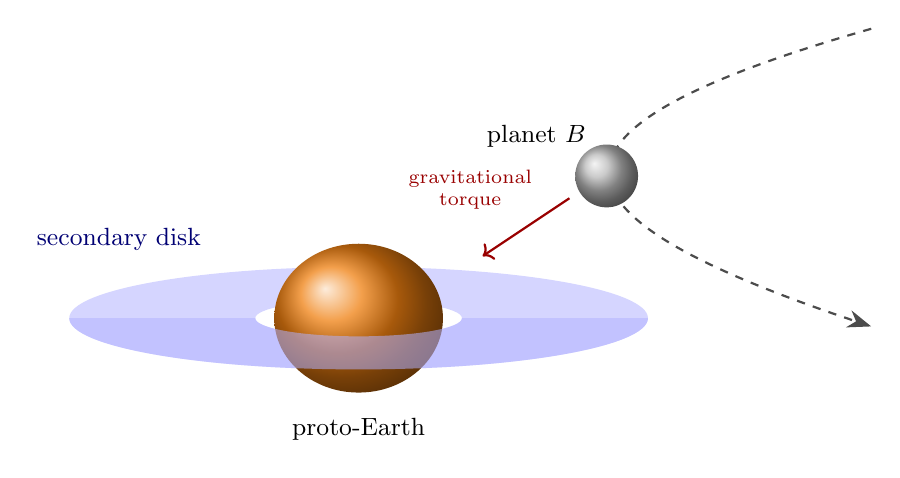
\begin{tikzpicture}[scale=1.05]
  \fill[blue!30,opacity=0.55,even odd rule] (0,0) ellipse (3.5 and 0.62) (0,0) ellipse (1.25 and 0.22);
  \shade[ball color=orange!75!brown] (0,0) ellipse (1.02 and 0.9);
  \begin{scope}
    \clip (-4,-1.2) rectangle (4,0);
    \fill[blue!30,opacity=0.55,even odd rule] (0,0) ellipse (3.5 and 0.62) (0,0) ellipse (1.25 and 0.22);
  \end{scope}
  \draw[dashed,thick,gray!60!black,-{Stealth[length=3mm]}]
      (6.2,3.5) .. controls (2.0,2.3) and (2.0,1.3) .. (6.2,-0.1);
  \shade[ball color=gray!55] (3.0,1.72) circle (0.38);
  \node[font=\small] at (2.15,2.2) {planet $B$};
  \node[font=\small] at (0,-1.35) {proto-Earth};
  \node[font=\small,blue!45!black] at (-2.9,0.95) {secondary disk};
  \draw[->,thick,red!60!black] (2.55,1.45) -- (1.5,0.75);
  \node[font=\scriptsize,red!60!black,align=center] at (1.35,1.55) {gravitational\\torque};
\end{tikzpicture}

\vspace{1.2cm}
{\large\bfseries Michel Debailleul\par}
\vspace{0.15cm}
Geophysicist, Independent Researcher --- Université libre de Bruxelles (ULB)\\
ORCID: 0009-0003-1222-1433 \quad | \quad \href{mailto:michel.debailleul@yahoo.fr}{michel.debailleul@yahoo.fr}\\[4pt]
\copyright\ 2026 Michel Debailleul --- License: CC BY-NC 4.0
\vfill
\end{titlepage}
\pagenumbering{roman}

% =====================================================================
%  ABSTRACT
% =====================================================================
\thispagestyle{plain}
\begin{center}{\Large\bfseries Abstract}\end{center}
\medskip

The Earth--Moon system currently exhibits a dynamical architecture, a mass distribution, an
angular momentum, isotopic signatures, geochemical compositions and a chronology that together
form independent observational constraints. The question addressed here is not to describe these
properties, but to identify a continuous \emph{physical path} linking the initial state of the
proto-terrestrial system to the observed state.

The astrophysical anchor of this approach is that natural satellites are already interpreted as
the products of circumplanetary reservoirs: the regular satellites of Jupiter and Saturn in
circumplanetary disks, and the inner satellites of Neptune in a reworked system where a debris
disk probably followed the capture of Triton. The proposed terrestrial case does not import their
masses or compositions; it retains the physical principle of a reservoir bound to a planet, able
to transport mass and angular momentum and then to form satellites.

This work explores such a path. A secondary circumterrestrial disk, contemporaneous with the
accretion of the proto-Earth, forms an orbital reservoir of mass and angular momentum before the
Moon forms. A planet $B$, on a grazing and non-collisional passage, is neither an impactor nor the
main supplier of lunar material: it acts as a \emph{transient gravitational agent redistributing
mass and angular-momentum fluxes} between four reservoirs --- the proto-Earth, the disk, planet
$B$ and the external medium.

The heliocentric logic of the model is that $B$ need not survive in the present Solar System. It may
belong to the population of primordial planetary bodies later eliminated by the global orbital
instability of the Solar System. This extension does not necessarily identify it with a fifth ice
giant; it only requires its grazing passage to precede its dynamical elimination, according to
$t_B<t_{\mathrm{ej}}$. It thus links the Earth--Moon problem to the broader problem of primordial
planetary migration and instability
\cite{Tsiganis2005,Gomes2005,Nesvorny2011,NesvornyMorbidelli2012,Liu2022,Clement2018}.

The passage performs an orbital sorting. A bound cohort of matter acquires an angular momentum
that places it, after circularization, beyond the Roche limit, in the window where the Moon can
accrete; one fraction re-accretes onto the proto-Earth, another escapes. A passage parallel to the
dynamical low-latitude band of an oblate rapidly rotating proto-Earth can also inject into the disk
surface material already depleted in metal and siderophile elements; W, V, Cr, Mn, FeO, O and Ti
then provide tracers with which to test the lineage.

The work successively formulates the scientific problem, the astrophysical foundations, the
reservoir architecture, the physical chronology, the passage dynamics, the evolution of the
circumterrestrial reservoir, geochemistry by tracer families, the viability domain and the
predictions, each with a verification method. It does not claim to prove a unique history: it
defines a quantitative and falsifiable physical path.

\bigskip
\noindent\textbf{Keywords:} Moon formation; circumterrestrial disk; secondary accretion;
non-collisional encounter; orbital sorting; angular momentum; Roche limit; lunar geochemistry; primordial orbital instability; eliminated planet.


% =====================================================================
%  METHODOLOGICAL PREAMBLE
% =====================================================================
\clearpage
\thispagestyle{plain}
\phantomsection
\addcontentsline{toc}{chapter}{Methodological preamble}
\begin{center}
{\Large\bfseries Methodological Preamble}\\[4pt]
{\large\bfseries A Retrodictive Path Theory}
\end{center}
\medskip

This monograph does not claim to reconstruct uniquely what actually happened
in the history of the Solar System. Such a reconstruction is probably
inaccessible: the exact initial conditions of the proto-terrestrial system, the
individual trajectories of planetary bodies, the detailed thermodynamic states
of the reservoirs, and the fine chronology of encounters have disappeared.

The aim is different. The purpose is to construct a \emph{possible physical
path} linking an admissible proto-terrestrial system to the observed
Earth--Moon system. The approach is therefore retrodictive: it starts from the
known final state and moves backward, constraint after constraint, toward a
family of initial states and dynamical steps capable of producing that final
state.

The problem addressed here is therefore not:

\begin{center}
\emph{Which unique event actually occurred?}
\end{center}

but rather:

\begin{center}
\emph{Does there exist a continuous, quantitatively constrained and falsifiable
physical path linking a possible proto-terrestrial state to the observed
Earth--Moon state?}
\end{center}

This status may be written as
\begin{equation}
\boxed{
\exists\,\Gamma(t)\in\mathcal{D}_{\mathrm{viable}}
\quad\text{such that}\quad
\Gamma(t_0)=\mathcal{S}_0,\qquad
\Gamma(t_f)=\mathcal{S}_f .
}
\label{eq:retrodictive-status}
\end{equation}

The trajectory $\Gamma(t)$ does not necessarily denote the real history of the
Solar System. It denotes an admissible path in the space of physical states:
mass, angular momentum, energy, composition, phases of matter, and chronology.
The scientific value of the theory therefore does not rest on a claim of
historical uniqueness, but on the possible existence of a continuous domain of
parameters satisfying, simultaneously, the dynamical, geochemical, isotopic,
thermodynamic and chronological constraints.

In this framework, the secondary circumterrestrial disk is not introduced as a
narrative device, but as a physical reservoir to be tested. Likewise, planet
$B$ is neither an impactor nor a main supplier of lunar material: it is a
transient gravitational agent redistributing mass and angular-momentum fluxes.
Its subsequent fate belongs to the same retrodictive framework. It may belong
to the population of planetary bodies of the primitive Solar System later
removed by collision, accretion, gravitational scattering or ejection.

The minimal condition associated with this heliocentric extension is
\begin{equation}
\boxed{
B\in\mathcal{P}_{\mathrm{elim}},
\qquad
 t_B<t_{\mathrm{ej}} .
}
\label{eq:B-elim-preamble}
\end{equation}

Here, $\mathcal{P}_{\mathrm{elim}}$ denotes the population of planetary bodies
present in the primitive Solar System but absent from the present one; $t_B$ is
the time of the grazing passage near the proto-Earth; and $t_{\mathrm{ej}}$ is
the time of the dynamical removal of $B$. This formulation leaves open both
possibilities: an early orbital instability or a later instability.

\begin{principe}{Status of the theory}
The theory of the secondary circumterrestrial disk is a path theory, not a
claim of historical uniqueness. It becomes credible if a continuous domain of
parameters allows the dynamical, geochemical, isotopic, thermodynamic and
chronological gates to be crossed together. It is falsified if no such domain
exists.
\end{principe}

% =====================================================================
%  READING GUIDE
% =====================================================================
\clearpage
\thispagestyle{plain}
\begin{center}{\Large\bfseries Reading guide}\end{center}
\medskip

The work is built to be read, not merely consulted. Each part begins with the question it
addresses and ends by linking to the next one. Long demonstrations are collected in
Appendix~\ref{app:demo}, so that the main text remains continuous; notation is collected in
Appendix~\ref{app:notations}, and numerical values in Appendix~\ref{app:constantes}.

Distinct kinds of boxes guide the reading:

\begin{definition}
Defines the meaning of a term or a role, which then becomes the reference for the whole work.
\end{definition}
\begin{ideephys}
Gives the physical intuition behind a calculation.
\end{ideephys}
\begin{lecture}
Interprets an equation or result within the physical path.
\end{lecture}
\begin{rappel}
Recalls a classical notion needed for understanding.
\end{rappel}
\begin{controle}
Compares a result with orders of magnitude or with a conservation balance.
\end{controle}
\begin{consequence}
States what should be observed, in lunar samples or simulations, if the described mechanism is at work.
\end{consequence}
\begin{falsif}
States the condition under which a branch of the theory must be abandoned.
\end{falsif}
\begin{apport}
Highlights what distinguishes the theory from existing scenarios.
\end{apport}

\clearpage
\tableofcontents

% =====================================================================
\clearpage
\pagenumbering{arabic}
\part{The scientific problem}
% =====================================================================

\noindent
This first part states the question answered by the work. It begins neither with the disk nor with
planet $B$, but with the Earth--Moon system as it is observed, and with the requirement these
observations impose on any account of its formation. The secondary disk, planet $B$, fluxes between
reservoirs, geochemistry and dynamics then appear as elements of a single answer.

% ---------------------------------------------------------------------
\chapter{From the proto-terrestrial system to the Earth--Moon system}
\label{ch:probleme}
% ---------------------------------------------------------------------

\section{The scientific problem}

The Moon exists. The Earth--Moon system currently has a dynamical architecture, a mass
distribution, an angular momentum, isotopic signatures, geochemical compositions and a chronology
that constitute independent observational constraints.

These observations are now numerous and precise enough to impose a demanding physical framework
on any theory of lunar formation. None of these constraints can be considered in isolation:
orbital dynamics, geochemistry, isotopic systems, thermodynamics and chronology describe one and
the same physical system and must be explainable coherently.

The scientific question is therefore not whether the Moon exists or what its present properties
are, but to determine:

\begin{center}
\emph{What physical path naturally led from the proto-terrestrial system\\ to the presently observed
Earth--Moon system?}
\end{center}

In other words, the task is to identify a physically admissible evolution linking an initial state
of the proto-Earth to the final state represented by the Earth--Moon system, while simultaneously
respecting the constraints imposed by observations. This approach may be represented generally as
\begin{equation}
\boxed{\;\mathcal{S}_0\longrightarrow\mathcal{S}_f\;}
\label{eq:S0Sf}
\end{equation}
where $\mathcal{S}_0$ denotes the initial state of the proto-terrestrial system and
$\mathcal{S}_f$ the currently observed state. The scientific problem is to determine whether a
continuous physical path exists between these two states.

\begin{figure}[htbp]
\centering
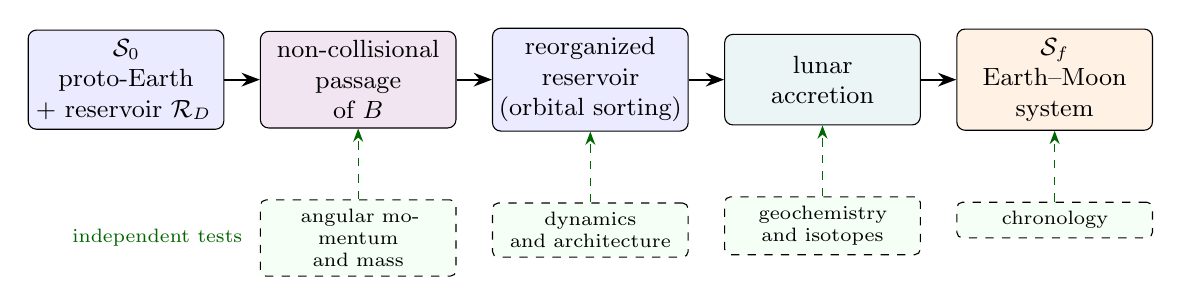
\begin{tikzpicture}[node distance=0.45cm,
  st/.style={draw,rounded corners=3pt,align=center,font=\small,minimum height=1.15cm,
             text width=2.25cm,fill=#1},
  st/.default=white,
  ts/.style={draw,dashed,rounded corners=2pt,align=center,font=\scriptsize,text width=2.25cm,
             fill=green!4}]
  \node[st=blue!8] (s0) {$\mathcal{S}_0$\\proto-Earth\\+ reservoir $\RD$};
  \node[st=violet!10,right=of s0] (s1) {non-collisional\\passage\\of $B$};
  \node[st=blue!8,right=of s1] (s2) {reorganized\\reservoir\\(orbital sorting)};
  \node[st=teal!8,right=of s2] (s3) {lunar\\accretion};
  \node[st=orange!10,right=of s3] (sf) {$\mathcal{S}_f$\\Earth--Moon\\system};
  \foreach \a/\b in {s0/s1,s1/s2,s2/s3,s3/sf} \draw[-{Stealth},thick] (\a) -- (\b);
  \node[ts,below=0.9cm of s1] (t1) {angular momentum\\and mass};
  \node[ts,below=0.9cm of s2] (t2) {dynamics\\and architecture};
  \node[ts,below=0.9cm of s3] (t3) {geochemistry\\and isotopes};
  \node[ts,below=0.9cm of sf] (t4) {chronology};
  \foreach \t/\s in {t1/s1,t2/s2,t3/s3,t4/sf} \draw[-{Stealth},dashed,green!40!black] (\t) -- (\s);
  \node[font=\scriptsize,green!40!black,anchor=east] at ($(t1.west)+(-0.1,0)$) {independent tests};
\end{tikzpicture}
\caption{The problem formulated as the search for a continuous physical path between the initial
state $\mathcal{S}_0$ and the observed state $\mathcal{S}_f$. Each family of observations tests the
path independently.}
\label{fig:chemin}
\end{figure}

\section{Observational constraints}

Table~\ref{tab:contraintes} gathers the families of constraints that the path must satisfy
simultaneously. They will serve, in Part~\ref{part:predictions}, as independent tests.

\begin{table}[htbp]
\centering
\small
\caption{Families of observational constraints imposed on the physical path.}
\label{tab:contraintes}
\begin{tabularx}{\textwidth}{>{\raggedright\arraybackslash}p{2.6cm}
>{\raggedright\arraybackslash}X >{\raggedright\arraybackslash}p{5.4cm}}
\toprule
\textbf{Family} & \textbf{Constraint} & \textbf{Nature or order of magnitude} \\
\midrule
Mass & ratio $M_L/\Mt$ & $1.23\times10^{-2}$ \\
Architecture & one dominant satellite & $f_{\mathrm{dom}}\simeq1$ \\
Angular momentum & total system angular momentum & $L_{\mathrm{EM}}\approx3.5\times10^{34}$ kg\,m$^2$\,s$^{-1}$ \\
Orbit & lunar orbital inclination & about $5^\circ$ relative to the ecliptic \\
Internal structure & small lunar core & at most a few percent of the mass \\
Isotopes & O, Ti, Cr, W & Earth and Moon very close, often indistinguishable \\
Siderophiles & V, Cr, Mn, W & depletions similar to those of Earth's mantle \\
Iron & FeO in the lunar mantle & higher than in Earth's mantle \\
Volatiles & K/U, Zn, isotopes & Moon depleted in volatile elements \\
Chronology & formation age & several tens of millions of years after the first solids \\
\bottomrule
\end{tabularx}
\end{table}


\section{Astrophysical anchor: natural satellites from disks}

Before introducing the terrestrial case, one astrophysical fact must be stated explicitly: the
formation of satellites from a circumplanetary reservoir is not an ad hoc construction. In the
Solar System, several families of natural satellites are interpreted as the products of matter
bound to a planet, organized in a disk, a massive ring or a debris disk, and then transformed into
satellites by accretion, migration, dissipation and crossing of the Roche limit.

\begin{principe}{Observational anchor}
The theory does not start from the abstract idea that a disk could form a Moon. It starts from a
principle observed more than once:
\begin{equation}
\boxed{\;\text{growing or reworked planet}+\text{circumplanetary reservoir}
\longrightarrow \text{natural satellites}.\;}
\label{eq:ancrage-satellites}
\end{equation}
The terrestrial case must then be treated with its own constraints: a terrestrial planet, a
solid-dominated reservoir, a high lunar mass and the non-collisional passage of $B$ acting as the
agent of redistribution.
\end{principe}

Three examples play a particular role in the reasoning. The Galilean system of Jupiter is the
classical example of a regular satellite system whose formation is linked to a circumjovian disk
fed during the growth of the planet. Models discuss gas and solid inflow, angular-momentum
transport, migration and the conditions of satellite accretion
\cite{CanupWard2002,MosqueiraEstrada2003a,CanupWard2006,Nimmo2026}. Saturn provides a second
anchor: its regular satellites and ring system show that a circumplanetary reservoir can transport
matter, spread viscously, cross the Roche limit and form satellites
\cite{Charnoz2010,CridaCharnoz2012,Blanc2025}. Neptune is subtler: Triton is very probably a
captured object, but its arrival may have destroyed or reworked a prior regular system and
produced a debris disk from which the present inner satellites reformed or reaccreted
\cite{AgnorHamilton2006,BanfieldMurray1992,Showalter2019,Szulagyi2018,Davis2026}.

\begin{table}[htbp]
\centering
\small
\caption{Natural examples showing that a circumplanetary reservoir can form or reform satellites.
These examples establish the physical principle; they do not set the parameters of the terrestrial
case.}
\label{tab:ancrage-satellites}
\begin{tabularx}{\textwidth}{>{\raggedright\arraybackslash}p{2.4cm}
>{\raggedright\arraybackslash}X >{\raggedright\arraybackslash}X}
\toprule
\textbf{System} & \textbf{Reservoir or process invoked} & \textbf{Physical lesson for the proposed path} \\
\midrule
Jupiter & circumjovian disk fed by gas and solids during the growth of Jupiter &
a circumplanetary disk can produce several organized regular satellites \\
Saturn & circumplanetary disk, massive rings, viscous spreading and crossing of the Roche limit &
a particulate reservoir can migrate, cross Roche and feed satellite accretion \\
Neptune & capture of Triton, destruction or reworking of a previous system, debris disk and
reaccretion of the inner satellites &
an external gravitational event can reorganize a circumplanetary system and leave a reservoir from
which satellites reform \\
\bottomrule
\end{tabularx}
\end{table}

This distinction is essential. The satellites of Jupiter, Saturn and Neptune do not prove the
history of the Moon. They show that nature already possesses the basic mechanism: storing matter
in a circumplanetary reservoir, transporting angular momentum within it and converting part of
that reservoir into satellites. The proposed theory applies this principle to the proto-terrestrial
case and adds its own step: the grazing non-collisional passage of $B$, which does not create the
reservoir but sorts and reorganizes it.

\section{Hypothesis explored}

The present theory explores one possible path. It applies to the proto-terrestrial case the
physical principle established by natural satellite systems: a planet can possess a
circumplanetary reservoir able to store matter, transport angular momentum and form satellites.
It is based on the hypothesis that a secondary circumterrestrial disk, contemporaneous with the
accretion of the proto-Earth, formed such an orbital reservoir of matter and angular momentum
before the Moon formed.

In this framework, a planetary body $B$ is neither an impactor nor the main supplier of lunar
material. Its passage remains non-collisional and acts as a transient gravitational agent that
redistributes mass and angular-momentum fluxes between the different reservoirs of the
proto-terrestrial system.

\begin{definition}
\textbf{Role of planet $B$.} Planet $B$ is a \emph{transient gravitational agent redistributing mass
and angular-momentum fluxes between the reservoirs of the proto-terrestrial system}. It is neither
an impactor nor the main supplier of lunar material. Its action begins and ends with its passage.
This definition is the reference for the entire work.
\end{definition}

The Moon then results from the evolution of this reorganized system, mainly from matter already
present in the circumterrestrial disk, possibly enriched by a limited contribution from the
superficial layers of the proto-Earth.

\section{Heliocentric fate of \texorpdfstring{$B$}{B} and eliminated planet}
\label{sec:destinB}

Defining $B$ as a transient agent immediately raises a legitimate question: if a planet grazed the
proto-Earth without colliding with it, where is it today? The theory answers by connecting the
Earth--Moon problem to the global evolution of the primordial Solar System. $B$ need not be a body
that still survives; it may belong to the population of planetary bodies eliminated during the
primordial orbital instabilities.

We denote this population by
\begin{equation}
\mathcal{P}_{\mathrm{elim}}=
\left\{\begin{array}{l}
\text{primordial planetary bodies eliminated by collision, accretion,}\\
\text{gravitational diffusion or ejection}
\end{array}\right\}.
\label{eq:Pelim}
\end{equation}
The minimal heliocentric proposal is therefore
\begin{equation}
\boxed{\;B\in\mathcal{P}_{\mathrm{elim}},\qquad t_B<t_{\mathrm{ej}}\;}
\label{eq:tB-tej}
\end{equation}
where $t_B$ is the time of the grazing passage near the proto-Earth, and $t_{\mathrm{ej}}$ is the time
of the ejection or dynamical elimination of $B$.

This formulation is deliberately more robust than the strong statement ``$B$ is the missing
planet''. Models of outer Solar System instability show that migration of the giant planets could
have reshaped the planetary architecture \cite{Tsiganis2005,Gomes2005}. Five- or six-planet
versions invoke the ejection of an additional planet, often an ice giant
\cite{Nesvorny2011,NesvornyMorbidelli2012}. Other work places the instability much earlier, at the
dispersal of the gaseous disk, and shows that growing terrestrial planets can be sculpted by such
an instability \cite{Liu2022,Clement2018}. The theory therefore does not choose, at this stage,
between an early and a later instability: it only requires that the Earth--$B$ passage belong to
$B$'s history before its elimination.

\begin{ideephys}
Planet $B$ is not an artificial object added only to the Earth--Moon problem. It may be understood
as a temporary member of the primordial Solar System: it passes near the proto-Earth, reorganizes
the circumterrestrial reservoir, and then rejoins the global heliocentric dynamics that removes
part of the excess planetary population. The grazing passage and the later disappearance of $B$
thus become two possible stages of the same history.
\end{ideephys}

The complete path then takes the form
\begin{equation}
\boxed{\begin{gathered}
B_{\mathrm{proto}}\longrightarrow\text{grazing passage near the proto-Earth}
\longrightarrow\mathcal{D}_1\\
\longrightarrow\text{heliocentric diffusion}
\longrightarrow\text{elimination of }B.
\end{gathered}}
\label{eq:cheminB}
\end{equation}
This extension does not replace the central mechanism of the theory. It gives it a wider logic:
the secondary disk and orbital sorting explain lunar formation, while primordial orbital
instability provides a natural fate for the transient agent $B$.

\section{Scope of the theory}

This theory is not presented as the unique possible history of lunar formation. Its objective is
more limited and more precise: to determine whether the proposed physical path defines a parameter
domain compatible with the full set of currently known dynamical, geochemical, isotopic,
thermodynamic and chronological constraints.

The observations are therefore not treated as presumed validations, but as independent tests that
can confirm, restrict or falsify the plausibility domain of the model.

Thus, even if all these constraints were satisfied simultaneously, the result would establish the
existence of a viable and quantitatively coherent physical path among possible scenarios for the
formation of the Moon, without claiming to demonstrate a unique history.

\begin{ideephys}
The object of the theory is the physical path. The disk is an initial condition, $B$ is the agent
of the transformation, the fluxes between reservoirs are the language, and geochemistry and
dynamics are the tests. Each part of the work answers one aspect of the same question:
\emph{how could the observed Earth--Moon system have emerged through a physically coherent
evolution?}
\end{ideephys}

\section{Scientific positioning of the proposed path}

The proposed path combines two elements with different status.

The \emph{secondary disk} belongs to an established framework. The idea that a circumterrestrial
reservoir contemporaneous with accretion could be the site of lunar formation is the idea of
co-accretion models \cite{Ruskol1960,Weidenschilling1986}, and the general principle of secondary
accretion is illustrated by natural satellite systems (Chapter~\ref{sec:satellites}).

The \emph{grazing non-collisional passage of a planet $B$} is the theory's own element. In giant
impact scenarios \cite{HartmannDavis1975,CameronWard1976,CanupAsphaug2001,Canup2004} and in
their high-angular-momentum variants \cite{CukStewart2012,Canup2012,Lock2018}, the disk is
produced by the collision, which also supplies the system angular momentum. In the proposed path,
the disk exists before the encounter, and $B$ acts on it through its gravitational field.
Table~\ref{tab:scenarios} locates the main scenario families according to a few descriptive
criteria.

\begin{table}[htbp]
\centering
\footnotesize
\setlength{\tabcolsep}{3pt}
\caption{Families of lunar-formation scenarios described according to four criteria.}
\label{tab:scenarios}
\begin{tabularx}{\textwidth}{>{\raggedright\arraybackslash}p{2.7cm}
>{\raggedright\arraybackslash}X >{\raggedright\arraybackslash}X
>{\raggedright\arraybackslash}X >{\raggedright\arraybackslash}X}
\toprule
\textbf{Scenario} & \textbf{Circumterrestrial reservoir} & \textbf{External body} &
\textbf{Nature of the interaction} & \textbf{Dominant lunar material} \\
\midrule
Canonical giant impact & created by the collision & impactor & collision &
mostly from the impactor \\[3pt]
High-angular-momentum impacts & created by the collision & impactor & collision &
mostly proto-terrestrial \\[3pt]
Co-accretion & contemporaneous with accretion & none & --- & circumterrestrial swarm \\[3pt]
Disruptive capture \cite{Mitler1975} & produced by disruption of the body & external body &
tidal disruption & external body \\[3pt]
Proposed path & preexisting, contemporaneous with accretion & planet $B$ &
grazing gravitational passage, without contact & reservoir and proto-Earth \\
\bottomrule
\end{tabularx}
\end{table}

\begin{lecture}
In the proposed path, a gravitational interaction occupies the role attributed to a collision in
impact scenarios. $B$ retains its physical identity and passes by. Its passage introduces an
external torque able to redistribute the angular momentum of the preexisting reservoir and to
reorganize it.
\end{lecture}

\section{Organization of the work}

The work follows the physical path in the order imposed by the question (Figure~\ref{fig:plan}).
Part~\ref{part:fondements} establishes the astrophysical foundations: secondary accretion around
planets is a real and recurrent phenomenon. Part~\ref{part:architecture} defines the four
reservoirs and the laws governing their exchanges. Part~\ref{part:chronologie} orders the path by
its time scales. Part~\ref{part:dynamique} describes the action of $B$ and its central result,
orbital sorting. Part~\ref{part:reservoir} follows the circumterrestrial reservoir before and after
the passage. Part~\ref{part:geochimie} organizes geochemical tests by families of tracers.
Part~\ref{part:viabilite} gathers the parameters, gates and numerical program. Part~\ref{part:predictions}
states the predictions in the form: \emph{if the theory is correct... here is how to verify it}.
The heliocentric fate of $B$ runs through these parts as a coherence constraint: the gravitational
agent must be able to pass near Earth and then be subsequently diffused or eliminated without
remaining in the present planetary architecture.

\begin{figure}[htbp]
\centering
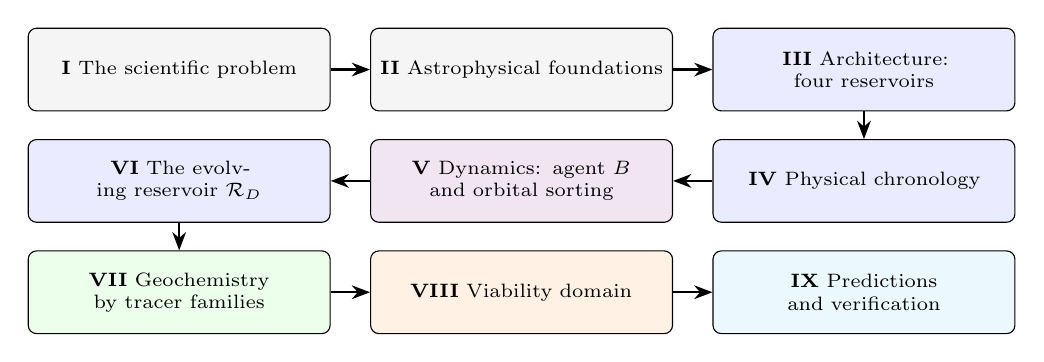
\begin{tikzpicture}[node distance=0.35cm and 0.5cm,
  pt/.style={draw,rounded corners=3pt,align=center,font=\scriptsize,minimum height=1.05cm,
             text width=3.6cm,fill=#1},pt/.default=white]
  \node[pt=gray!8] (p1) {\textbf{I} The scientific problem};
  \node[pt=gray!8,right=of p1] (p2) {\textbf{II} Astrophysical foundations};
  \node[pt=blue!8,right=of p2] (p3) {\textbf{III} Architecture: four reservoirs};
  \node[pt=blue!8,below=of p3] (p4) {\textbf{IV} Physical chronology};
  \node[pt=violet!10,left=of p4] (p5) {\textbf{V} Dynamics: agent $B$ and orbital sorting};
  \node[pt=blue!8,left=of p5] (p6) {\textbf{VI} The evolving reservoir $\RD$};
  \node[pt=green!8,below=of p6] (p7) {\textbf{VII} Geochemistry by tracer families};
  \node[pt=orange!10,right=of p7] (p8) {\textbf{VIII} Viability domain};
  \node[pt=cyan!8,right=of p8] (p9) {\textbf{IX} Predictions and verification};
  \foreach \a/\b in {p1/p2,p2/p3,p3/p4,p4/p5,p5/p6,p6/p7,p7/p8,p8/p9}
    \draw[-{Stealth},thick] (\a) -- (\b);
\end{tikzpicture}
\caption{Architecture of the work: each part answers one aspect of the same question.}
\label{fig:plan}
\end{figure}

% =====================================================================
\part{Astrophysical foundations}
\label{part:fondements}
% =====================================================================

\noindent
Before proposing a path for the Earth, the first element of that path must be shown to belong to
known physics. This part shows that secondary accretion around planets is a real and recurrent
phenomenon, while specifying what the analogies do and do not allow. It ends with the specificity
of the terrestrial case: a solid-dominated disk whose feeding mode differs from that of giant
planets.

% ---------------------------------------------------------------------
\chapter{The principle of secondary accretion}
\label{ch:accretion-secondaire}\label{sec:satellites}
% ---------------------------------------------------------------------

\section{The circumplanetary principle}

Natural satellite systems provide a direct anchor for the notion of a secondary accretion system.
The large regular satellites of Jupiter, Saturn and Uranus are mostly prograde, weakly eccentric
and organized around their planet's equatorial plane or Laplace plane. They are dynamical archives
of circumplanetary evolution \cite{Nimmo2026,Blanc2025,JPL}. The following systems are retained as
reference examples.

\begin{table}[htbp]
\centering
\caption{Satellite systems used as support for the principle of circumplanetary accretion. The
comparison concerns the physical principle of the disk, not an identity of mass or thermodynamics
with the proto-Earth.}
\label{tab:systemes}
\begin{tabular}{ll}
\toprule
\textbf{Planet} & \textbf{Satellites considered} \\
\midrule
Jupiter & Io, Europa, Ganymede, Callisto \\
Saturn & Mimas, Enceladus, Tethys, Dione, Rhea, Titan, Iapetus \\
Uranus  & Miranda, Ariel, Umbriel, Titania, Oberon \\
\bottomrule
\end{tabular}
\end{table}

Models for the formation of regular satellites explicitly treat matter supply, angular-momentum
transport, cooling, migration and accretion within a disk surrounding the central planet
\cite{CanupWard2002,CanupWard2006,Nimmo2026}.

\begin{ideephys}
The theory does not transpose to the proto-Earth the disk mass of Jupiter or Saturn. It retains a
more fundamental result: a growing planetary body may be surrounded by a rotating reservoir that
transports mass and angular momentum and can become the site of satellite accretion.
\end{ideephys}

\section{Physical meaning of the term ``secondary''}

The disk is called secondary relative to the primary circumsolar disk. The hierarchy of the two
accretion systems is
\begin{equation}
\text{primary circumsolar disk}\longrightarrow\text{proto-Earth}\longrightarrow
\text{secondary circumterrestrial disk.}
\label{eq:hierarchie}
\end{equation}
The word ``secondary'' describes a gravitational and accretional hierarchy. It does not mean that
the disk appears late, nor that it is created by planet $B$.

\section{Three nested propositions}

The theory distinguishes three logical levels in order to separate general disk physics, what
natural systems show, and what constitutes the specifically terrestrial proposition.

\begin{principe}{Principle of secondary circumplanetary accretion}
\textbf{P1 --- General physics.} A growing planet can receive matter carrying angular momentum and
organize a fraction of it into a rotating circumplanetary reservoir. This reservoir transports mass
and angular momentum and can become a site of satellite accretion \cite{Pringle1981,CanupWard2002,CanupWard2006}.

\smallskip
\textbf{P2 --- Natural manifestations.} The regular systems of Jupiter, Saturn and Uranus are
natural expressions of secondary circumplanetary accretion. Their detailed histories differ from
one system to another, but their architecture requires that matter bound to the planet was
organized and accreted in its orbital environment \cite{Nimmo2026,Blanc2025,Helled2020}.

\smallskip
\textbf{P3 --- Terrestrial proposition.} The proto-Earth possessed a secondary circumterrestrial disk
when planet $B$ grazed it without collision. This encounter reorganized the reservoir and prepared
the accretion of a dominant satellite: the Moon.
\end{principe}

This separation protects the logic of the theory. The Jovian, Saturnian and Uranian systems show
several physical realizations of the same general principle; the terrestrial branch must then be
computed with the parameters proper to the proto-Earth and with the specific perturbation by $B$.

\section{A hierarchy of accretion systems}

The general hierarchy is
\begin{equation}
\text{circumstellar disk}\to\text{growing planet}\to
\text{circumplanetary disk}\to\text{satellites}
\label{eq:hierarchie-gen}
\end{equation}
The proposed terrestrial case is
\begin{equation}
\text{circumsolar disk}\rightarrow\text{proto-Earth + secondary disk}
\xrightarrow{\;\text{passage of }B\;}\text{reorganized disk}\rightarrow\text{Moon}.
\label{eq:hierarchie-terre}
\end{equation}

\begin{figure}[htbp]
\centering
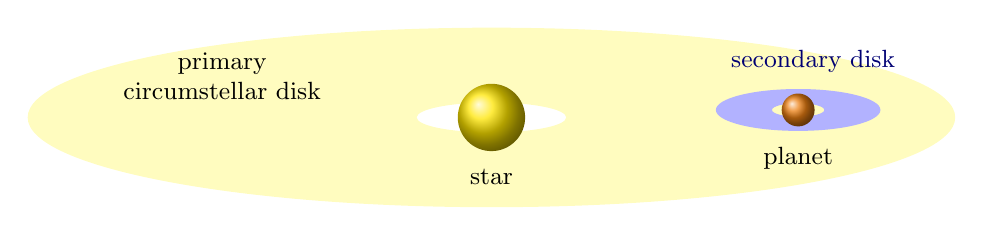
\begin{tikzpicture}[scale=0.95]
  \fill[yellow!25,even odd rule] (0,0) ellipse (6.2 and 1.2) (0,0) ellipse (1.0 and 0.2);
  \shade[ball color=yellow!80!orange] (0,0) circle (0.45);
  \node[font=\small] at (0,-0.8) {star};
  \fill[blue!30,even odd rule] (4.1,0.1) ellipse (1.1 and 0.28) (4.1,0.1) ellipse (0.35 and 0.09);
  \shade[ball color=orange!70!brown] (4.1,0.1) circle (0.22);
  \node[font=\small] at (4.1,-0.55) {planet};
  \node[font=\small,blue!45!black] at (4.3,0.75) {secondary disk};
  \node[font=\small,align=center] at (-3.6,0.55) {primary\\circumstellar disk};
\end{tikzpicture}
\caption{Principle of secondary accretion: the circumplanetary disk is an accretion system nested
inside the primary circumstellar system.}
\label{fig:hierarchie}
\end{figure}

\section{Jupiter: the Galilean system as a dynamical reference}

Io, Europa, Ganymede and Callisto form a compact system of prograde satellites with eccentricities
of order $10^{-3}$ to $10^{-2}$ and small inclinations relative to Jupiter's Laplace plane
\cite{JPL}. This organization is consistent with accretion in a dissipative disk able to damp
random motions.

The recent review of the Galilean system \cite{Nimmo2026} identifies as major uncertainties the
distribution of angular momentum in the matter feeding the disk, the origin of solids, and the
thermal and viscous structure of the disk. These are precisely the quantities that describe the
circumterrestrial disk:
\begin{equation}
\mathcal{V}_D=\left\{\dot M_{\mathrm{in}},\ \Sigma(r,t),\ T(r,t),\ \nu(r,t),\ L_D(t),\
\mathbf{X}(r,t)\right\}.
\label{eq:VD}
\end{equation}
The density gradient of the Galilean satellites, with an ice fraction increasing outward, shows
that a satellite-forming disk imprints radial thermochemical information on the bodies that form
within it. The function $T(r,t)$ must therefore be treated as a variable of material formation, not
only as a dynamical parameter.

\section{Saturn: viscous transport, Roche limit and satellite birth}

Large moons such as Titan and Iapetus can be related to an ancient circumplanetary phase; Iapetus,
which is more inclined than the inner satellites, is retained as a dynamically distinct limiting
case. The ring environment illustrates another mechanism: a particulate reservoir spreads
viscously and forms small satellites when a fraction of its matter crosses the Roche limit
\cite{Charnoz2010,Blanc2025}:
\begin{equation}
\text{circumplanetary reservoir}\to\text{spreading}\to
\text{Roche crossing}\to\text{satellite accretion}
\label{eq:saturne}
\end{equation}
This sequence is directly useful for the terrestrial case: the Roche limit does not fix the inner
edge of the disk; it marks a transition in the ability of matter to build durable self-gravitating
aggregates.

\section{Uranus: a regular system with a still-debated reservoir origin}

Miranda, Ariel, Umbriel, Titania and Oberon form a regular system organized around Uranus's
equator. The exact origin of this reservoir remains debated: models of a primordial
circumplanetary disk and of a disk produced later have been proposed \cite{Helled2020,Blanc2025}.
Uranus is therefore used as an example of the accretion principle in a circumplanetary reservoir,
without imposing an identity of origin with the terrestrial reservoir.


\section{Neptune: Triton's capture, debris disk and reaccretion}

Neptune does not provide the same type of evidence as Jupiter or Saturn. Its dominant satellite,
Triton, is retrograde and strongly inclined; it is therefore generally interpreted as a captured
body, probably through a gravitational encounter involving a trans-Neptunian binary
\cite{AgnorHamilton2006}. This capture profoundly reworked the Neptunian system.

The important point for the present theory is not Triton itself, but Neptune's inner satellites.
In the scenario of Banfield and Murray, Triton's highly eccentric post-capture orbit excites the
former inner satellites, drives collisions, forms a debris disk, and then leaves an inner system of
satellites to reform on nearly equatorial orbits \cite{BanfieldMurray1992}. The discovery and
analysis of Hippocamp reinforce the picture of a young, fragmented and reassembled inner system,
strongly shaped by collisions \cite{Showalter2019}. Simulations of satellite formation around ice
giants further show that Uranus and Neptune can form circumplanetary disks capable of producing
regular satellite systems; Neptune may therefore have possessed an initially Uranus-like system
before Triton's reworking \cite{Szulagyi2018}. Recent JWST observations of Neptune's rings and
inner moons even suggest that their material may come from the interiors of older icy bodies that
were destroyed or reworked \cite{Davis2026}.

\begin{ideephys}
The Neptunian case provides an analogy different from those of Jupiter and Saturn. It shows that
an external gravitational event can destroy, sort or reorganize circumplanetary matter, then leave
a reservoir from which inner satellites reform. In the proposed terrestrial path, $B$ neither
captures the Moon nor supplies its main mass; nevertheless it plays the analogous role of a
gravitational agent of reorganization.
\end{ideephys}

\section{Direct observation: the circumplanetary disk of PDS 70c}

ALMA has resolved around the young planet PDS~70c a compact dust source spatially separated from
the circumstellar disk and interpreted as a circumplanetary disk \cite{Benisty2021}. The system
provides a direct observation of two nested levels of accretion:
\begin{equation}
\text{circumstellar disk of PDS~70}\ \supset\ \text{PDS~70c}+\text{circumplanetary disk}.
\label{eq:pds70}
\end{equation}

\begin{ideephys}
PDS~70c shows that a planet still in formation can possess its own disk inside a larger
circumstellar disk. The theory transposes this hierarchy principle to the proto-Earth, then adds
the perturbation specific to it: the non-collisional passage of $B$.
\end{ideephys}

% ---------------------------------------------------------------------
\chapter{From the principle to the terrestrial case}
\label{ch:cas-terrestre}
% ---------------------------------------------------------------------

Natural systems establish the principle; they do not fix terrestrial values. This chapter
quantitatively compares satellite systems, formulates the constraint of a dominant satellite, and
identifies the nature of the terrestrial disk.

\section{Quantitative comparison of natural systems}

The satellite mass fraction is defined as
\begin{equation}
\mu_{\mathrm{sat}}=\frac{\sum_i M_i}{M_p}.
\label{eq:musat}
\end{equation}
Using the gravitational parameters from JPL \cite{JPL}, one obtains the values in
Table~\ref{tab:musat}.

\begin{table}[htbp]
\centering
\caption{Mass fraction of the selected satellite systems, computed from $GM$ parameters
(independent of the adopted value of $G$).}
\label{tab:musat}
\begin{tabular}{llc}
\toprule
\textbf{System} & \textbf{Satellites included} & $\mu_{\mathrm{sat}}$ \\
\midrule
Jupiter & Io, Europa, Ganymede, Callisto & $2.07\times10^{-4}$ \\
Saturn & Mimas, Enceladus, Tethys, Dione, Rhea, Titan, Iapetus & $2.47\times10^{-4}$ \\
Uranus  & Miranda, Ariel, Umbriel, Titania, Oberon & $1.04\times10^{-4}$ \\
Earth   & Moon & $1.23\times10^{-2}$ \\
\bottomrule
\end{tabular}
\end{table}

\begin{figure}[htbp]
\centering
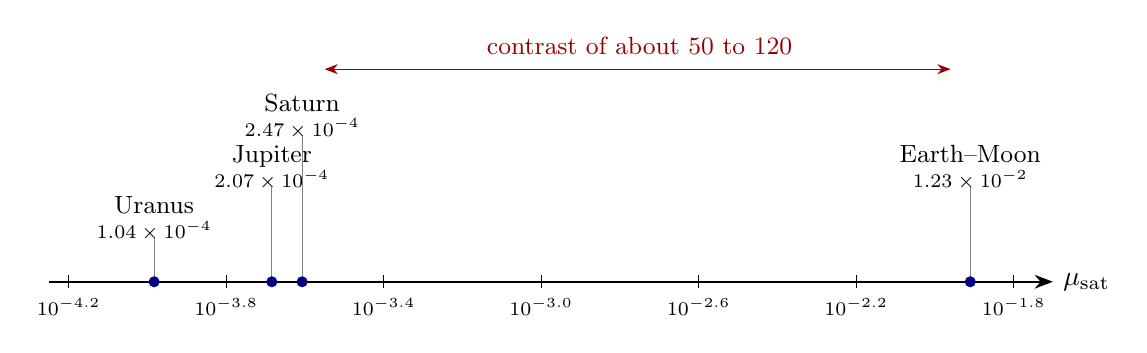
\begin{tikzpicture}[x=5cm,y=1cm]
  \draw[thick,-{Stealth}] (-4.25,0) -- (-1.7,0) node[right] {$\mu_{\mathrm{sat}}$};
  \foreach \e/\lab in {-4.2/{-4.2},-3.8/{-3.8},-3.4/{-3.4},-3.0/{-3.0},-2.6/{-2.6},-2.2/{-2.2},-1.8/{-1.8}}
    \draw (\e,0.08) -- (\e,-0.08) node[below,font=\scriptsize] {$10^{\lab}$};
  \foreach \x/\y/\n/\v in {-3.983/0.8/Uranus/{1.04\times10^{-4}},-3.684/1.45/Jupiter/{2.07\times10^{-4}},-3.607/2.1/Saturn/{2.47\times10^{-4}},-1.910/1.45/{Earth--Moon}/{1.23\times10^{-2}}}{
    \draw[gray] (\x,0) -- (\x,\y-0.25);
    \fill[blue!50!black] (\x,0) circle (2pt);
    \node[font=\small,align=center] at (\x,\y) {\n\\[-2pt]{\scriptsize$\v$}};
  }
  \draw[{Stealth}-{Stealth},red!60!black] (-3.55,2.7) -- (-1.96,2.7);
  \node[font=\small,red!60!black] at (-2.75,3.0) {contrast of about 50 to 120};
\end{tikzpicture}
\caption{Mass contrast between the regular systems of the giant planets and the Earth--Moon system
(logarithmic scale). This contrast is a quantitative constraint on the terrestrial case, not an
objection to the circumplanetary principle.}
\label{fig:contraste}
\end{figure}

The three giant-planet systems lie at order $10^{-4}$, consistent with the regulation regime
described for continuously fed gaseous disks \cite{CanupWard2006}. The mass contrast is defined as
\begin{equation}
C_M=\frac{M_L/\Mt}{\mu_{\text{sat,giant}}},
\qquad 50\lesssim C_M\lesssim 120.
\label{eq:CM}
\end{equation}

\begin{controle}
This difference does not refute the principle of secondary accretion. It defines a constraint
specific to the terrestrial case: the circumterrestrial disk, reorganized by $B$, must produce a
satellite mass outcome far more concentrated than the regular systems of the giant planets. The
theory must quantitatively explain why a lunar-mass dominant satellite emerges from the terrestrial
system.
\end{controle}

\section{From several satellites to one dominant satellite}

A simple measure of satellite mass concentration is
\begin{equation}
f_{\mathrm{dom}}=\frac{M_{\max}}{\sum_i M_i}.
\label{eq:fdom}
\end{equation}
In the present terrestrial system, $f_{\mathrm{dom}}\simeq1$. The specific dynamical role of $B$ is
expressed as
\begin{equation}
\mathcal{D}_0\xrightarrow{\;B\;}\mathcal{D}_1
\xrightarrow{\;\text{dissipation + accretion}\;}\left\{M_L,\ f_{\mathrm{dom}}\simeq1\right\}.
\label{eq:roleB}
\end{equation}

\begin{falsif}
If, in the parameter domain that respects the other constraints, the post-encounter disk
systematically produces several satellites of comparable mass or a total satellite mass far below
the lunar mass, the proposed reorganization mechanism is insufficient.
\end{falsif}

\section{Specificity of the terrestrial case: a solid-dominated disk}
\label{sec:soustherm}

Jupiter, Saturn and PDS~70c exceed the \emph{thermal mass} of their disk,
\begin{equation}
M_{\mathrm{th}}\simeq\left(\frac{H}{r}\right)^{3}M_\odot\approx10\,\Mt
\quad\text{at 1 AU},
\label{eq:Mth}
\end{equation}
beyond which captured gas forms a rotating disk. The proto-Earth, ten times less massive, lies in
the \emph{sub-thermal} regime. Its Bondi radius,
\begin{equation}
R_{\mathrm{B}}=\frac{G\Mt}{c_s^2}\approx4.0\times10^{8}\ \mathrm{m}\approx63\,\Rt
\qquad(T\approx280\ \mathrm{K},\ \mu=2.34),
\label{eq:Bondi}
\end{equation}
is smaller than its Hill radius ($\approx235\,\Rt$), and therefore fixes the accretion zone; high
resolution simulations show that pebbles crossing the Bondi sphere of a rocky embryo are indeed
accreted \cite{Popovas2018}.

The circularization radius of matter with specific angular momentum
$j\simeq\Omega R_{\mathrm{acc}}^2/4$ is $r_c=j^2/(G\Mt)$ \cite{QuillenTrilling1998}:
\begin{equation}
r_c(R_{\mathrm{acc}}=R_H)=\frac{R_H}{48}\approx4.9\,\Rt,
\qquad
r_c(R_{\mathrm{acc}}=R_{\mathrm{B}})=\left(\frac{R_{\mathrm{B}}}{R_H}\right)^{4}
\frac{R_H}{48}\approx0.03\,\Rt.
\label{eq:rc}
\end{equation}
Nebular gas captured through the Bondi sphere therefore falls back onto the planet rather than
forming a disk, in agreement with simulations of sub-thermal embryo envelopes supported by
pressure rather than rotation \cite{Ormel2015,Fung2015}. The terrestrial secondary disk is
therefore dominated by solids, with three feeding channels:
\begin{equation}
\dot M_{\mathrm{in}}=\dot M_{\mathrm{coacc}}+\dot M_{\mathrm{ej}}+\dot M_{\mathrm{rot}},
\label{eq:canaux}
\end{equation}
where $\dot M_{\mathrm{coacc}}$ represents capture by collisions of planetesimals within the Hill
sphere \cite{Ruskol1960,Weidenschilling1986}, $\dot M_{\mathrm{ej}}$ ordinary accretion-impact
ejecta, and $\dot M_{\mathrm{rot}}$ equatorial mass loss from a proto-Earth rotating close to the
critical limit.

\begin{lecture}
The analogy with giant planets concerns the principle of a circumplanetary reservoir, not its mode
of supply. The rotational channel $\dot M_{\mathrm{rot}}$ is the one most directly coupled to the
rest of the theory: it supplies material of terrestrial silicate composition, oriented by the spin,
and links the fast rotation of the proto-Earth to the very existence of the disk.
\end{lecture}

% =====================================================================

\begin{rappel}
Part~\ref{part:fondements} has established two results. First, a rotating circumplanetary reservoir
is a real astrophysical object. Second, in the terrestrial case this reservoir is dominated by
solids and must produce a satellite mass concentrated in one body. The next part translates these
results into a common physical language: reservoirs and fluxes.
\end{rappel}

% =====================================================================
\part{Physical architecture: the four reservoirs}
\label{part:architecture}
% =====================================================================

\noindent
The physical path is described as a sequence of exchanges between reservoirs. This language has a
decisive advantage: it requires the balances of mass, angular momentum, energy and composition to
be closed at every step, and it gives the role of $B$ a precise formulation. This part defines the
reservoirs, the fluxes connecting them and the conservation laws that constrain them, then fixes
the Level~I state variables and numerical reference scales.

% ---------------------------------------------------------------------
\chapter{Reservoirs, fluxes and conservation laws}
\label{ch:reservoirs}
% ---------------------------------------------------------------------

\section{The four reservoirs of the system}

The proto-terrestrial system is decomposed into four reservoirs:
\begin{equation}
\mathcal{R}=\left\{\RT,\ \RD,\ \RB,\ \Rinf\right\}.
\label{eq:reservoirs}
\end{equation}

\begin{definition}
\textbf{$\RT$} --- the proto-Earth: its mass, spin, internal structure and the composition of its
layers.\\
\textbf{$\RD$} --- the secondary circumterrestrial reservoir: gaseous, multiphase or particulate disk,
and the population of aggregates or moonlets it contains.\\
\textbf{$\RB$} --- planet $B$: its mass, spin and orbital motion relative to the proto-Earth.\\
\textbf{$\Rinf$} --- the external medium not bound to the Earth--disk system: heliocentric matter
entering the system (co-accretion) or leaving it (escape).
\end{definition}

Each reservoir $i$ is described by a state
\begin{equation}
\mathcal{X}_i=\left\{M_i,\ \mathbf{J}_i,\ E_i,\ \mathbf{X}_i\right\},
\label{eq:etat-reservoir}
\end{equation}
which gathers its mass, angular momentum, energy and composition. Angular momenta are defined in
the barycentric frame of the system:
\begin{equation}
\mathbf{J}_\oplus=\mathbf{S}_\oplus,\qquad
\mathbf{J}_D=\mathbf{L}_D+\sum_k\mathbf{L}_k,\qquad
\mathbf{J}_B=\mathbf{S}_B+\mathbf{L}_{\mathrm{orb}},\qquad
\mathbf{J}_\infty=\mathbf{L}_{\mathrm{esc}},
\label{eq:J-reservoirs}
\end{equation}
where $\mathbf{L}_k$ is the orbital angular momentum of moonlets and $\mathbf{L}_{\mathrm{orb}}$ that of
the relative Earth--$B$ motion.

\begin{figure}[htbp]
\centering
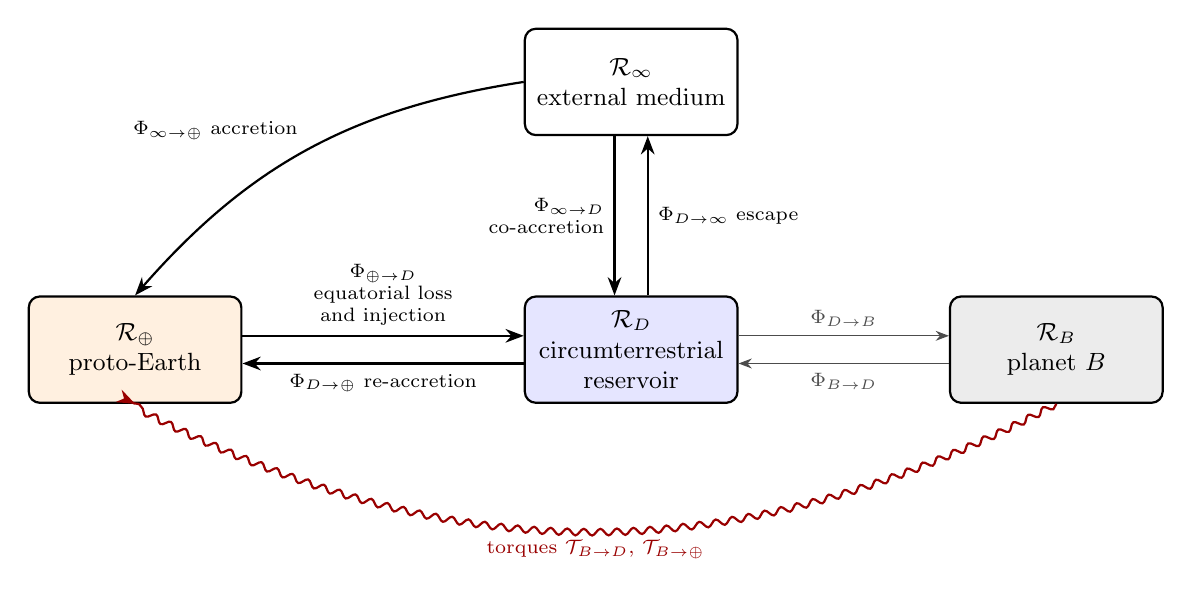
\begin{tikzpicture}[
  rs/.style={draw,thick,rounded corners=4pt,align=center,font=\small,minimum width=2.7cm,
             minimum height=1.35cm,fill=#1},rs/.default=white]
  \node[rs=orange!12] (T) at (0,0) {$\RT$\\proto-Earth};
  \node[rs=blue!10] (D) at (6.3,0) {$\RD$\\circumterrestrial\\reservoir};
  \node[rs=gray!15] (B) at (11.7,0) {$\RB$\\planet $B$};
  \node[rs=white] (I) at (6.3,3.4) {$\Rinf$\\external medium};
  \draw[-{Stealth},thick] ([yshift=5pt]T.east) -- node[above,font=\scriptsize,align=center]{$\Phi_{\oplus\to D}$\\equatorial loss\\and injection} ([yshift=5pt]D.west);
  \draw[-{Stealth},thick] ([yshift=-5pt]D.west) -- node[below,font=\scriptsize]{$\Phi_{D\to\oplus}$ re-accretion} ([yshift=-5pt]T.east);
  \draw[-{Stealth},thick] ([xshift=-6pt]I.south) -- node[left,font=\scriptsize,align=right]{$\Phi_{\infty\to D}$\\co-accretion} ([xshift=-6pt]D.north);
  \draw[-{Stealth},thick] ([xshift=6pt]D.north) -- node[right,font=\scriptsize]{$\Phi_{D\to\infty}$ escape} ([xshift=6pt]I.south);
  \draw[-{Stealth},thick] (I.west) to[bend right=20] node[above left,font=\scriptsize]{$\Phi_{\infty\to\oplus}$ accretion} (T.north);
  \draw[-{Stealth},gray!60!black] ([yshift=5pt]D.east) -- node[above,font=\scriptsize]{$\Phi_{D\to B}$} ([yshift=5pt]B.west);
  \draw[-{Stealth},gray!60!black] ([yshift=-5pt]B.west) -- node[below,font=\scriptsize]{$\Phi_{B\to D}$} ([yshift=-5pt]D.east);
  \draw[red!60!black,thick,decorate,decoration={snake,amplitude=1.2pt,segment length=6pt},-{Stealth}]
     (B.south) to[bend left=28] node[below,font=\scriptsize]{torques $\mathcal{T}_{B\to D}$, $\mathcal{T}_{B\to\oplus}$} (T.south);
\end{tikzpicture}
\caption{The four reservoirs and their exchanges. Solid arrows represent mass fluxes, carrying
angular momentum, energy and composition; the wavy arrow represents the gravitational torques exerted
by $B$ during its passage.}
\label{fig:reservoirs}
\end{figure}

\section{Mass fluxes}

Let $\Phi_{i\to j}\ge0$ denote the mass flux from reservoir $i$ to reservoir $j$. The evolution of
each reservoir is
\begin{equation}
\frac{\dd M_i}{\dd t}=\sum_{j\neq i}\left(\Phi_{j\to i}-\Phi_{i\to j}\right),
\qquad
\sum_i M_i=\text{constant}.
\label{eq:flux-masse}
\end{equation}
The principal fluxes are grouped in Table~\ref{tab:flux}. Equation~\eqref{eq:bilanM} for the disk
is the special case $i=D$ of this relation.

\begin{table}[htbp]
\centering
\small
\caption{Principal mass fluxes between reservoirs and associated processes.}
\label{tab:flux}
\begin{tabular}{lll}
\toprule
\textbf{Flux} & \textbf{Process} & \textbf{Dominant phase} \\
\midrule
$\Phi_{\infty\to\oplus}$ & growth of the proto-Earth & growth \\
$\Phi_{\infty\to D}$ & co-accretion, capture in the Hill sphere & growth \\
$\Phi_{\oplus\to D}^{\mathrm{rot}}$ & rotational equatorial mass loss & growth \\
$\Phi_{\oplus\to D}^{\mathrm{mar}}$ & injection by the tide of $B$ & encounter \\
$\Phi_{D\to\oplus}$ & re-accretion & encounter, relaxation \\
$\Phi_{D\to\infty}$ & escape & encounter, relaxation \\
$\Phi_{D\to B},\ \Phi_{B\to D}$ & capture by $B$, material ceded by $B$ & encounter \\
\bottomrule
\end{tabular}
\end{table}

\section{Angular momentum}

A mass flux carries the specific angular momentum $\mathbf{j}_{i\to j}$ of the transferred matter,
$\boldsymbol{\Lambda}_{i\to j}=\Phi_{i\to j}\,\mathbf{j}_{i\to j}$. Reservoirs also exchange angular
momentum through gravitational torques $\boldsymbol{\mathcal{T}}_{j\to i}$:
\begin{equation}
\frac{\dd\mathbf{J}_i}{\dd t}=\sum_{j\neq i}\left(\boldsymbol{\Lambda}_{j\to i}-\boldsymbol{\Lambda}_{i\to j}\right)
+\sum_{j\neq i}\boldsymbol{\mathcal{T}}_{j\to i},
\qquad
\boldsymbol{\mathcal{T}}_{j\to i}=-\boldsymbol{\mathcal{T}}_{i\to j}.
\label{eq:flux-J}
\end{equation}
Internal torques cancel pairwise, so that
\begin{equation}
\boxed{\;\sum_i\mathbf{J}_i=\text{constant}\;}
\label{eq:conservation-J}
\end{equation}
as long as the solar torque is negligible, which is the case during the encounter. The angular
momentum balance of the encounter (Chapter~\ref{ch:bilans}) is the direct application of this law.

\begin{ideephys}
In this language, the role of $B$ becomes exact. During its passage, the torques
$\boldsymbol{\mathcal{T}}_{B\to D}$ and $\boldsymbol{\mathcal{T}}_{B\to\oplus}$ dominate the other terms,
and they trigger the fluxes $\Phi_{\oplus\to D}$, $\Phi_{D\to\oplus}$ and $\Phi_{D\to\infty}$. When
$B$ moves away, these terms vanish: this is the meaning of \emph{transient} in the definition of
$B$.
\end{ideephys}

\section{Energy}

Mechanical energy is not conserved along the path: the relaxation of the reservoir converts
orbital energy into heat, which is then radiated. The global balance is
\begin{equation}
\frac{\dd}{\dd t}\left(\sum_iE_i+E_{\mathrm{int}}+E_{\mathrm{th}}\right)=-\mathcal{L}_{\mathrm{rad}},
\label{eq:energie}
\end{equation}
where $E_{\mathrm{int}}$ is the gravitational interaction energy between reservoirs,
$E_{\mathrm{th}}$ the thermal energy, and $\mathcal{L}_{\mathrm{rad}}$ the radiated power.
Dissipation by shocks, collisions and viscosity, detailed in Chapter~\ref{ch:reorganisation}, is
the source term for $E_{\mathrm{th}}$.

\section{Composition}

Each flux carries a composition $\mathbf{X}_{i\to j}$ that is not necessarily that of the mean
reservoir: it depends on the depth, latitude and phase of the transferred matter. The composition
of each reservoir evolves according to
\begin{equation}
\frac{\dd(M_i\mathbf{X}_i)}{\dd t}=\sum_{j\neq i}\left(\Phi_{j\to i}\mathbf{X}_{j\to i}
-\Phi_{i\to j}\mathbf{X}_{i\to j}\right)+\boldsymbol{\Pi}_i,
\label{eq:flux-X}
\end{equation}
where $\boldsymbol{\Pi}_i$ represents internal transformations within the reservoir: melting,
condensation, evaporation, metal segregation.

\begin{lecture}
Equation~\eqref{eq:flux-X} is the entry point of geochemistry. The flux
$\Phi_{\oplus\to D}^{\mathrm{mar}}$ samples matter from a specific layer of the proto-Earth; its
composition $\mathbf{X}_{\oplus\to D}$ therefore carries the memory of the latitude and depth from
which it was stripped. Part~\ref{part:geochimie} uses this memory.
\end{lecture}

\section{Level I state variables}

Level I characterizes the admissible state of the Earth--disk system just before the passage of
$B$, then measures its transformation during the encounter. Natural satellite systems define
classes of behavior to reproduce or distinguish: angular-momentum transport, cooling, crossing of
the Roche limit, migration, accretion and concentration of satellite mass.

The proto-terrestrial state is
\begin{equation}
\Psi_\oplus=\left\{\Mt,\ \Req,\ \Omega_\oplus,\ S_\oplus,\ T_\oplus(r),\ \rho_\oplus(r),\
\mathbf{X}_\oplus(r)\right\},
\label{eq:Psiterre}
\end{equation}
and the disk state is
\begin{equation}
\begin{aligned}
\mathcal{D}_0=\Big\{&M_{D,0},\ \Sigma_0(r),\ R_{\mathrm{in}},\ R_{\mathrm{out}},\ T_0(r),\
P_0(r),\ H_0(r),\\
&L_{D,0},\ v_{r,0}(r),\ \kappa_0(r),\ \mathbf{X}_0(r),\
\mathbf{f}_{\mathrm{phase},0}(r),\ \mathcal{G}_0\Big\},
\end{aligned}
\label{eq:D0}
\end{equation}
where $\mathcal{G}_0=\{m_k,a_k,e_k,i_k,\mathbf{X}_k\}_{k=1}^{N_0}$ describes the population of
aggregates or moonlets already formed at $t_B$ (Section~\ref{sec:regimes}). The vector of phase
fractions is
\begin{equation}
\mathbf{f}_{\mathrm{phase}}=(f_{\mathrm{vap}},f_{\mathrm{liq}},f_{\mathrm{sol}}),\qquad
f_{\mathrm{vap}}+f_{\mathrm{liq}}+f_{\mathrm{sol}}=1.
\label{eq:fphase}
\end{equation}

\section{Encounter parameters}

The state of $B$ is described by
\begin{equation}
\Psi_B=\left\{M_B,\ R_B,\ \rho_B,\ q_B,\ v_\infty,\ i_B,\ \omega_B,\ \varpi_B,\ \mathbf{S}_B\right\},
\label{eq:PsiB}
\end{equation}
where $q_B$ is the minimum geocentric distance of the nominal trajectory, $v_\infty$ the relative
asymptotic velocity, $i_B$ the inclination of the trajectory relative to the disk plane, $\omega_B$
the argument of periastron measured from the line of nodes, $\varpi_B$ the longitude of
periastron, and $\mathbf{S}_B$ the spin of $B$. The minimal parameter vector is
\begin{equation}
\Theta_I=\left\{\Psi_\oplus,\ \mathcal{D}_0,\ \Psi_B,\ t_B\right\}.
\label{eq:Theta}
\end{equation}
To connect the encounter to the later fate of $B$, we also define the heliocentric extension
\begin{equation}
\Theta_I^{+}=\left\{\Theta_I,\ \mathcal{H}_{B,1},\ t_{\mathrm{ej}}\right\},
\qquad
\mathcal{H}_{B,1}=\left\{a_{B,1},e_{B,1},i_{B,1},\Omega_{B,1},\omega_{B,1}\right\},
\label{eq:Theta-plus}
\end{equation}
where $\mathcal{H}_{B,1}$ denotes the heliocentric elements of $B$ after its passage near the
proto-Earth. This extension is not required to compute the local orbital sorting, but it becomes
necessary to test the connection with the global instability of the Solar System.

\begin{falsif}
Level I fails if no continuous domain of $\Theta_I$ simultaneously allows a physically persistent
preexisting disk, a non-collisional encounter, a closed angular-momentum balance, sufficient
post-encounter disk mass and a composition compatible with lunar constraints.
\end{falsif}

\section{Reference scales of the proto-Earth--disk--\texorpdfstring{$B$}{B} system}

Table~\ref{tab:echelles} gathers the numerical scales that bound Level I. They are computed for a
proto-Earth with present terrestrial mass and radius at 1~AU; the values associated with $B$
correspond to a reference case $M_B=0.1\,\Mt$, $q_B=2\,\Rt$, parabolic trajectory.

\begin{table}[htbp]
\centering
\small
\caption{Reference scales. These values are not solutions: they define the orders of magnitude
against which the outputs of the calculation must be placed.}
\label{tab:echelles}
\begin{tabular}{lll}
\toprule
\textbf{Quantity} & \textbf{Expression} & \textbf{Value} \\
\midrule
Hill radius & $a_\oplus(\Mt/3M_\odot)^{1/3}$ & $1.50\times10^{9}$ m $\approx235\,\Rt$ \\
Truncated outer edge & $\xi_H R_H$, $\xi_H\approx0.3$--$0.4$ & $\approx70$--$95\,\Rt$ \\
Thermal mass & $(H/r)^3M_\odot$ & $\approx10\,\Mt$ \\
Bondi radius & $G\Mt/c_s^2$ & $\approx63\,\Rt$ \\
Circularization (Hill) & $R_H/48$ & $\approx4.9\,\Rt$ \\
Circularization (Bondi) & $(R_{\mathrm{B}}/R_H)^4R_H/48$ & $\approx0.03\,\Rt$ \\
Roche limit ($\rho_s=3.34$ g\,cm$^{-3}$) & Eq.~\eqref{eq:Roche} & $1.85\times10^{7}$ m $\approx2.9\,\Rt$ \\
Orbital period at $\aR$ & $2\pi(\aR^3/G\Mt)^{1/2}$ & $\approx7.0$ h \\
Synchronous orbit ($P_\oplus=4$--$5$ h) & $(G\Mt/\Omega_\oplus^2)^{1/3}$ & $\approx2.0$--$2.3\,\Rt$ \\
Critical rotation period & $2\pi(\Rt^3/G\Mt)^{1/2}$ & $\approx1.4$ h \\
Critical spin ($k\approx0.33$) & $k\Mt\Rt^2\Omega_{\mathrm{c}}$ & $\approx1.0\times10^{35}$ kg\,m$^2$\,s$^{-1}$ \\
Present Earth--Moon angular momentum & $L_{\mathrm{EM}}$ & $\approx3.5\times10^{34}$ kg\,m$^2$\,s$^{-1}$ \\
Orbital angular momentum of one Moon at $\aR$ & $M_L(G\Mt\aR)^{1/2}$ & $\approx6.3\times10^{33}$ kg\,m$^2$\,s$^{-1}$ \\
Relative orbital angular momentum of $B$ & Eq.~\eqref{eq:LBrel} & $\approx5.7\times10^{34}$ kg\,m$^2$\,s$^{-1}$ \\
Periastron velocity of $B$ & $(2G\Mtot/q_B)^{1/2}$ & $\approx8.3$ km\,s$^{-1}$ \\
Characteristic encounter duration & $q_B/v_p$ & $\approx26$ min \\
Roche distance of $B$ ($\rho_B=3.93$ g\,cm$^{-3}$) & Eq.~\eqref{eq:RocheB} & $\approx2.75\,\Rt$ \\
\bottomrule
\end{tabular}
\end{table}

\begin{controle}
Three comparisons structure what follows. The relative orbital angular momentum carried by $B$ is
of the same order as the total angular momentum of the Earth--Moon system: without collision, a
grazing passage has an angular-momentum reservoir on the scale of the problem. The encounter
duration is short compared with the orbital period at the Roche limit: the disk undergoes an
impulsive forcing. Finally, the Roche distance of $B$ is close to the passage distances considered:
the integrity of $B$ becomes an explicit constraint.
\end{controle}

% =====================================================================
\part{Physical chronology}
\label{part:chronologie}
% =====================================================================

\noindent
The chronology is not narrated here as a sequence of episodes. It is constructed from physics: each
phase of the path is defined by the terms that dominate the flux equations~\eqref{eq:flux-masse}--\eqref{eq:flux-X},
and by its own time scale. The separation of these scales justifies dividing the calculation into
successive phases.

% ---------------------------------------------------------------------
\chapter{Physical chronology of the path}
\label{ch:chronologie}
% ---------------------------------------------------------------------

\section{Phases defined by dominant fluxes}

Table~\ref{tab:phases} defines the phases of the path by their dominant terms.

\begin{table}[htbp]
\centering
\small
\caption{Phases of the physical path, defined by the dominant terms of the flux equations.}
\label{tab:phases}
\begin{tabularx}{\textwidth}{>{\raggedright\arraybackslash}p{3.1cm}
>{\raggedright\arraybackslash}X >{\raggedright\arraybackslash}p{3.6cm}}
\toprule
\textbf{Phase} & \textbf{Dominant terms} & \textbf{Time scale} \\
\midrule
0 --- Growth and feeding & $\Phi_{\infty\to\oplus}$, $\Phi_{\infty\to D}$, $\Phi^{\mathrm{rot}}_{\oplus\to D}$, torques $\mathcal{T}_{\oplus\to D}$ & $10^{6}$--$10^{8}$ yr \\
I --- Pre-encounter state & viscous transport, accretion into aggregates and moonlets & $t_\nu$, $t_{\mathrm{sat}}$ \\
II --- Encounter & $\mathcal{T}_{B\to D}$, $\mathcal{T}_{B\to\oplus}$, $\Phi^{\mathrm{mar}}_{\oplus\to D}$ & $t_{\mathrm{enc}}\sim$ 0.5--2 h \\
III --- Sorting and relaxation & $\Phi_{D\to\oplus}$, $\Phi_{D\to\infty}$, dissipation & $10$--$10^{3}$ orbital periods \\
IV --- Lunar accretion & accretion beyond Roche, transport from the inner disk & months to $10^{2}$ yr \\
V --- Lunar magma ocean & cooling and differentiation of the Moon & $10^{7}$--$10^{8}$ yr \\
VI --- Fate of $B$ & heliocentric diffusion, planetary encounters, elimination or ejection & early or late instability \\
\bottomrule
\end{tabularx}
\end{table}

\section{Hierarchy of time scales}

The characteristic time scales are ordered as
\begin{equation}
\boxed{\;t_{\mathrm{enc}}<P_{\mathrm{orb}}(\aR)\ll t_{\mathrm{relax}}\lesssim t_{\mathrm{acc},L}
\ll t_{\mathrm{LMO}}\;}
\label{eq:hierarchie-temps}
\end{equation}
with $t_{\mathrm{enc}}\approx26$~min in the reference case and $P_{\mathrm{orb}}(\aR)\approx7$~h
(Table~\ref{tab:echelles}). Figure~\ref{fig:temps} places these scales on a logarithmic axis.

\begin{figure}[htbp]
\centering
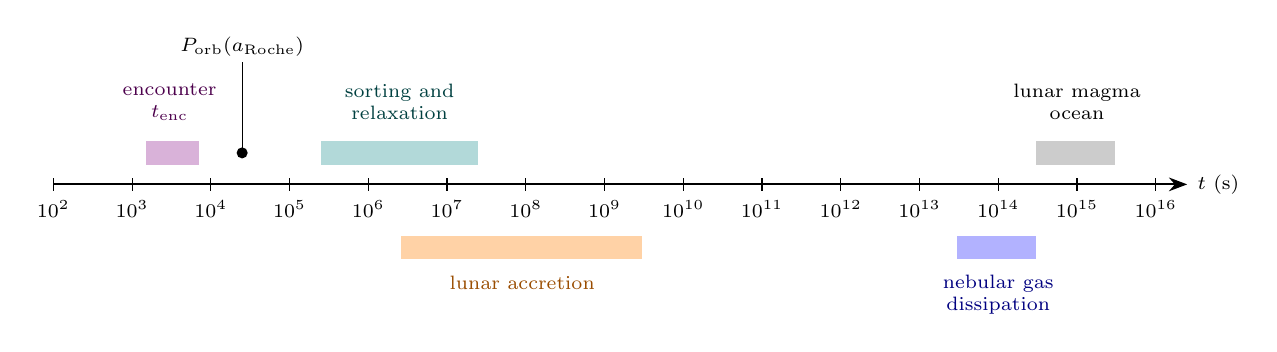
\begin{tikzpicture}[x=1cm,y=1cm]
  \draw[thick,-{Stealth}] (0,0) -- (14.4,0) node[right,font=\scriptsize] {$t$ (s)};
  \foreach \k in {2,...,16}{
    \pgfmathsetmacro{\xx}{\k-2}
    \draw (\xx,0.08) -- (\xx,-0.08) node[below,font=\scriptsize] {$10^{\k}$};}
  \fill[violet!30] (1.176,0.25) rectangle (1.845,0.55);
  \node[font=\scriptsize,violet!60!black,align=center] at (1.477,1.05) {encounter\\$t_{\mathrm{enc}}$};
  \fill[black] (2.398,0.4) circle (2pt);
  \node[font=\scriptsize,align=center] at (2.398,1.75) {$P_{\mathrm{orb}}(\aR)$};
  \draw[thin] (2.398,0.45) -- (2.398,1.55);
  \fill[teal!30] (3.398,0.25) rectangle (5.398,0.55);
  \node[font=\scriptsize,teal!50!black,align=center] at (4.398,1.05) {sorting and\\relaxation};
  \fill[orange!35] (4.415,-0.95) rectangle (7.477,-0.65);
  \node[font=\scriptsize,orange!60!black] at (5.954,-1.25) {lunar accretion};
  \fill[gray!40] (12.477,0.25) rectangle (13.477,0.55);
  \node[font=\scriptsize,align=center] at (13.000,1.05) {lunar magma\\ocean};
  \fill[blue!30] (11.477,-0.95) rectangle (12.477,-0.65);
  \node[font=\scriptsize,blue!50!black,align=center] at (12.000,-1.4) {nebular gas\\dissipation};
\end{tikzpicture}
\caption{Time scales of the physical path (order-of-magnitude values). Eleven orders of magnitude
separate the encounter duration from that of the lunar magma ocean.}
\label{fig:temps}
\end{figure}

\begin{ideephys}
The encounter lasts less than one orbital period at the Roche limit: during the passage, the
reservoir does not have time to evolve viscously and may be treated as frozen. After the passage,
relaxation extends over hundreds of periods, without further intervention by $B$. This separation
of scales justifies the division of the numerical program into Phases~A, B and C
(Chapter~\ref{ch:programme}).
\end{ideephys}

\section{Order of stages}

The minimal chronology is
\begin{equation}
t^{\mathrm{start}}_{\mathrm{accr},\oplus}<t^{\mathrm{form}}_D<t_B<t^{\mathrm{reorg}}_D
<t^{\mathrm{accr}}_L<t_{\mathrm{LMO}},
\label{eq:ordre}
\end{equation}
This chain fixes the internal order of the Earth--Moon problem. The heliocentric connection adds an
independent condition:
\begin{equation}
\boxed{\;t_B<t_{\mathrm{ej}}\;},
\label{eq:ordreB}
\end{equation}
without requiring $t_{\mathrm{ej}}$ to belong to either an early or a late instability. The calculation
must simply show that a post-passage orbit of $B$ can join a trajectory eliminated by global
dynamics.

and a more complete chronological vector is
\begin{equation}
\mathbf{t}=\left\{t^{\mathrm{form}}_D,\ t^{\mathrm{feed}}_D,\ t^{\mathrm{cool}}_D,\
t^{\mathrm{cond}}_D,\ t_B,\ t_{\mathrm{relax}},\ t_{\mathrm{Roche}},\
t^{\mathrm{start}}_{\mathrm{acc},L},\ t^{\mathrm{end}}_{\mathrm{acc},L},\ t_{\mathrm{LMO}},\ t_{\mathrm{ej}}\right\}.
\label{eq:vecteur-t}
\end{equation}

\section{Gaseous disk and residual reservoir}

The theory distinguishes the physical states of the circumterrestrial reservoir:
\begin{equation}
\mathcal{D}(t)=\mathcal{D}_{\mathrm{gas}}\cup\mathcal{D}_{\mathrm{multiphase}}\cup
\mathcal{D}_{\mathrm{particulate}},
\label{eq:etats}
\end{equation}
the weighting between these regimes being computed by $\mathbf{f}_{\mathrm{phase}}(r,t)$.

Nebular gas dissipates within a few million years, whereas lunar chronometers place the accretion
of the Moon several tens of millions of years after the formation of the first solids; rapid
growth of the proto-Earth by pebble accretion \cite{Johansen2021} and its later completion bound
the interval $[t^{\mathrm{start}}_{\mathrm{accr},\oplus},t_B]$. At the time of the passage, the
reservoir is therefore described by its multiphase and particulate components, fed by the channels
of Eq.~\eqref{eq:canaux}.

\begin{lecture}
This distinction prevents the theory from depending on the persistence of a gas-rich disk. The
reservoir evolves toward a multiphase or particulate state while conserving circumterrestrial mass
and angular momentum, and it is this state that the passage of $B$ reorganizes.
\end{lecture}

% =====================================================================

\section{Three chronological regimes}
\label{sec:regimes}

Let $t_{\mathrm{sat}}$ be the characteristic time of satellite accretion and
$\Delta t_{\mathrm{preB}}=t_B-t_{D,\mathrm{form}}$ the time available before the passage. We distinguish
\begin{align}
&\text{late accretion regime:} && t_{\mathrm{sat}}\gg\Delta t_{\mathrm{preB}},
\label{eq:tardif}\\
&\text{intermediate regime:} && t_{\mathrm{sat}}\sim\Delta t_{\mathrm{preB}},
\label{eq:interm}\\
&\text{early accretion regime:} && t_{\mathrm{sat}}\ll\Delta t_{\mathrm{preB}}.
\label{eq:precoce}
\end{align}

The available time scales orient this choice. An unfed gaseous component spreads in
\begin{equation}
t_\nu=\left[\alpha\,h^2\,\Omega_K\right]^{-1}\approx80\ \text{yr}
\qquad(\alpha=10^{-3},\ h=H/r=0.1,\ r=10\,\Rt),
\label{eq:tnu-num}
\end{equation}
and a particulate component located beyond the Roche limit aggregates in a few months to about a
year \cite{Ida1997,Kokubo2000}. These reference times are compared with
$\Delta t_{\mathrm{preB}}$ and the disk feeding rate; the calculation determines which of the three
regimes belongs to the viable domain. When the reservoir contains moonlets $\mathcal{G}_0$ at the
time of the passage, those located beyond $a_{\mathrm{sync}}$ migrate outward.

\begin{lecture}
When moonlets are present, the role of $B$ becomes more precise: by exciting eccentricities and
inclinations, it produces orbit crossings between moonlets and between moonlets and the residual
disk, and therefore mergers. The grazing passage becomes a mechanism for concentrating satellite
mass, giving physical content to the condition $f_{\mathrm{dom}}\to1$.
\end{lecture}

\begin{rappel}
The chronology has fixed the order and duration of the phases. The next part enters the shortest
and most decisive phase: the encounter, during which agent $B$ redistributes the mass and
angular-momentum fluxes.
\end{rappel}

% =====================================================================
\part{Dynamics: the gravitational agent \texorpdfstring{$B$}{B}}
\label{part:dynamique}
% =====================================================================

\noindent
This part is the original core of the theory. It describes how a planet $B$, without ever touching
the proto-Earth, redistributes mass and angular-momentum fluxes between reservoirs. It contains
four chapters: the passage itself and its low-latitude geometry, the injection of superficial
proto-terrestrial matter, the central result of the passage --- the orbital sorting that defines the
lunar window --- and finally the balances that close the encounter.

% ---------------------------------------------------------------------
\chapter{The non-collisional passage}
\label{ch:passage}\label{sec:passage}
% ---------------------------------------------------------------------

Consistently with its definition (Chapter~\ref{ch:probleme}), $B$ acts on the Earth--reservoir
system solely through its gravitational field. This chapter establishes the frequency of such
passages, their geometry, their dynamical regime and the exact force field they exert.

\section{A gravitational interaction without contact}

During the growth of terrestrial planets, planetary embryos cross one another and undergo many
close encounters. Including gravitational focusing, the cross-section for encounters whose
periastron is smaller than $q$ is
\begin{equation}
\sigma(q)=\pi q^2\left[1+\frac{2G\Mtot}{q\,v_\infty^2}\right],
\qquad \Mtot=\Mt+M_B.
\label{eq:sigma}
\end{equation}
Let $R_c=\Req+R_{B,\mathrm{eff}}$ be the contact distance and
$\Theta=2G\Mtot/(R_c v_\infty^2)$ the focusing parameter. The ratio between the number of grazing
passages ($R_c<q<2R_c$) and collisions ($q<R_c$) is
\begin{equation}
\frac{\mathcal{N}_{\mathrm{graze}}}{\mathcal{N}_{\mathrm{coll}}}
=\frac{\sigma(2R_c)-\sigma(R_c)}{\sigma(R_c)}
=\frac{3+\Theta}{1+\Theta}\ \in\ [1,\,3].
\label{eq:frequence}
\end{equation}

\begin{apport}
Grazing passages are at least as frequent as collisions, and up to three times more frequent when
gravitational focusing is weak. The mechanism of the theory therefore does not rely on an
exceptional event: it selects, from the natural population of planetary encounters, those that do
not end in contact. Non-collisional encounters are also recognized as an efficient process in early
Earth--Moon dynamics \cite{PahlevanMorbidelli2015}; the theory assigns them an earlier and more
fundamental role here: reorganizing the disk from which the Moon forms.
\end{apport}

\section{Geometrical definition of the non-collisional character}

The scenario is gravitational. The trajectory of $B$ does not touch the proto-Earth:
\begin{equation}
q_B>\Req+R_{B,\mathrm{eff}},
\label{eq:nc}
\end{equation}
where $\Req$ is the equatorial radius of the rotating proto-Earth, larger than the polar radius,
and $R_{B,\mathrm{eff}}$ is the radius of $B$ deformed by the terrestrial tide. The eccentricity of
the relative hyperbolic trajectory is
\begin{equation}
e_B=1+\frac{q_B\,v_\infty^2}{G\Mtot}.
\label{eq:eB}
\end{equation}
The trajectory crosses the disk plane at two nodes located at
\begin{equation}
r_{\text{node}}^{\pm}=\frac{q_B\,(1+e_B)}{1\pm e_B\cos\omega_B}.
\label{eq:noeuds}
\end{equation}
For configurations in which the theory requires $B$ not to cross the dense part of the disk, one
imposes
\begin{equation}
R_{\mathrm{out,dense}}<\min\left(r_{\text{node}}^{+},r_{\text{node}}^{-}\right)
=\frac{q_B\,(1+e_B)}{1+e_B\,|\cos\omega_B|}.
\label{eq:nontraversee}
\end{equation}
For a quasi-parabolic trajectory whose periastron is highest above the disk plane
($\omega_B=\pi/2$), this bound is $2q_B$.

\begin{lecture}
The action of $B$ is carried by its gravitational field. The inclined geometry allows a strong
perturbation of the disk while maintaining physical separation between $B$, the proto-Earth and
the dense part of the disk: a dense disk extending over a few Earth radii, consistent with the
circularization radius of Eq.~\eqref{eq:rc}, is entirely compatible with a passage at $q_B$ of a
few $\Rt$.
\end{lecture}

\section{Dynamical regime of the encounter}

The relative velocity at periastron and the characteristic duration of the encounter are
\begin{equation}
v_p=\sqrt{v_\infty^2+\frac{2G\Mtot}{q_B}},
\qquad
t_{\mathrm{enc}}\simeq\frac{q_B}{v_p}.
\label{eq:tenc}
\end{equation}
The response regime of a disk region at radius $r$ is measured by
\begin{equation}
\eta(r)=\Omega_K(r)\,t_{\mathrm{enc}}.
\label{eq:eta}
\end{equation}
For $\eta\ll1$ the response is impulsive, for $\eta\sim1$ it is resonant, and for $\eta\gg1$ it is
adiabatic and the forcing is attenuated. In the reference case of Table~\ref{tab:echelles},
$t_{\mathrm{enc}}\approx26$~min and $\eta(\aR)\approx0.4$: the region where the Moon assembles
receives an impulsive forcing. For the proto-Earth itself, the analogous parameter
$\eta_\oplus=\Omega_\oplus t_{\mathrm{enc}}$ is of order unity when the rotation is close to the
critical limit: the tide of $B$ then acts on a time scale close to the rotation period, which
strengthens the coupling between the passage and equatorial matter.

\section{Exact differential field}

In a frame centered on the proto-Earth, the exact differential acceleration due to $B$ on a parcel
located at $\mathbf{r}$ is
\begin{equation}
\mathbf{a}_{B,\mathrm{diff}}=-GM_B\left[
\frac{\mathbf{r}-\mathbf{r}_B(t)}{|\mathbf{r}-\mathbf{r}_B(t)|^3}
+\frac{\mathbf{r}_B(t)}{|\mathbf{r}_B(t)|^3}\right].
\label{eq:adiff}
\end{equation}
The first term is the direct attraction by $B$, the second the acceleration of the proto-Earth
itself toward $B$ (indirect term). This expression is used without multipolar expansion in the
grazing regime, where $|\mathbf{r}|$ and $|\mathbf{r}_B|$ are comparable.

\section{Torque exerted on the disk}

The total torque of $B$ on the disk and the resulting change in angular momentum are
\begin{equation}
\boldsymbol{\mathcal{T}}_{B\to D}=\int_D\mathbf{r}\times\mathbf{a}_{B,\mathrm{diff}}\,\dd m,
\qquad
\Delta\mathbf{L}_D=\int_{t_i}^{t_f}\boldsymbol{\mathcal{T}}_{B\to D}\,\dd t+\Delta\mathbf{L}_{\mathrm{flux}},
\label{eq:couple}
\end{equation}
where $\Delta\mathbf{L}_{\mathrm{flux}}$ represents the angular momentum transported by matter that
enters or leaves the disk during the encounter. The main dynamical outputs are
\begin{equation}
\mathcal{O}_B=\left\{\Delta M_D,\ \Delta\mathbf{L}_D,\ \Delta e_D,\ \Delta i_D,\
\Delta R_{\mathrm{out}},\ \Delta T_D,\ \Delta\mathcal{G}\right\}.
\label{eq:OB}
\end{equation}

\section{Low-latitude geometry of the passage}
\label{sec:low-latitude}

The geometry retained by the theory is a passage \emph{parallel to the dynamical low-latitude
band} of an oblate, rapidly rotating proto-Earth, in the direction of its rotation. It combines four
favorable effects.

\paragraph{Targeted latitude.}
At periastron, the point of the proto-Earth vertically below $B$ lies at latitude
\begin{equation}
\lambda_B=\arcsin\left(\sin i_B\,\sin\omega_B\right),
\label{eq:lambdaB}
\end{equation}
where $i_B$ is the inclination of the trajectory relative to the rotational equator and $\omega_B$
the argument of periastron. The low-latitude passage condition is
\begin{equation}
|\lambda_B|\le\lambda_c,
\label{eq:low-latitude}
\end{equation}
that is, $i_B\lesssim\lambda_c$ for $\omega_B=90^\circ$. The quantity $\lambda_c$ defines a
dynamical low-latitude band around the instantaneous rotational equator of the proto-Earth. Its
value is not imposed by the present obliquity; it is determined by the coupling between rotation,
oblateness, the tide of $B$ and the response of the reservoir.

\paragraph{Equatorial forcing is preserved.}
The radial tidal acceleration varies as $(3\cos^2\psi-1)$, where $\psi$ is the angle from the
sub-$B$ point. At the equator, at the longitude of the targeted point, $\psi=\lambda_B$ and the
relative forcing is
\begin{equation}
F(\lambda_B)=\frac{3\cos^2\lambda_B-1}{2},
\qquad F(20^\circ)\approx0.82.
\label{eq:Flambda}
\end{equation}
A slight inclination therefore costs little equatorial forcing.

\paragraph{Oblateness strengthens the action of \texorpdfstring{$B$}{B}.}
For an oblate proto-Earth, the equatorial effective gravity is, to first order in $J_2$,
\begin{equation}
g_{\mathrm{eff,eq}}=\frac{G\Mt}{\Req^2}\left(1+\frac32J_2\right)-\Omega_\oplus^2\Req.
\label{eq:geffJ2}
\end{equation}
The injection threshold (Chapter~\ref{ch:injection}) contains the factor $(\Req/q_B)^3$: an
equatorial radius larger by 10 to 20\% increases the tidal term by 33 to 73\%, precisely where the
effective gravity is weakest.

\paragraph{The prograde sense prolongs the forcing.}
If $B$ passes in the direction of the proto-Earth's rotation, the same longitude remains longer
under the tidal bulge. With $\Omega_B=v_p/q_B$ the angular velocity of $B$ at periastron, the ratio
of the prograde and retrograde forcing durations is
\begin{equation}
\frac{\tau_{\mathrm{pro}}}{\tau_{\text{retro}}}=\frac{\Omega_\oplus+\Omega_B}{\Omega_\oplus-\Omega_B}.
\label{eq:prograde}
\end{equation}
For $q_B=3\,\Rt$, $\Omega_B\approx3.5\times10^{-4}$~rad\,s$^{-1}$; for a proto-Earth close to
critical rotation, $\Omega_\oplus\approx1.2\times10^{-3}$~rad\,s$^{-1}$, and the ratio is about
$1.8$. This mechanism is the planetary analogue of the efficiency of prograde encounters shown in
galaxies \cite{ToomreToomre1972}.

\paragraph{The geometry remains compatible with non-crossing of the dense disk.}
With $\omega_B=90^\circ$, $B$ passes at periastron at height $q_B\sin i_B$ above the equatorial
plane and crosses that plane only at nodes located at about $2q_B$ (Eq.~\eqref{eq:noeuds}). A dense
reservoir extending to $5\,\Rt$ is not crossed once $q_B\gtrsim2.5\,\Rt$.

\begin{figure}[htbp]
\centering
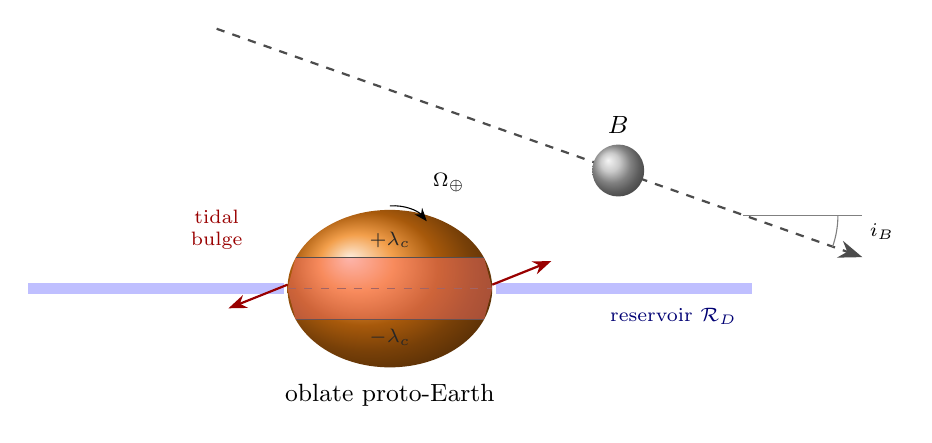
\begin{tikzpicture}[scale=1.0]
  \fill[blue!25] (-4.6,-0.07) rectangle (-1.35,0.07);
  \fill[blue!25] (1.35,-0.07) rectangle (4.6,0.07);
  \shade[ball color=orange!75!brown] (0,0) ellipse (1.3 and 1.0);
  \draw[dashed,gray!70!black] (-1.3,0) -- (1.3,0);
  \draw[gray!60!black] ({-1.3*cos(asin(0.39))},0.39) -- ({1.3*cos(asin(0.39))},0.39);
  \draw[gray!60!black] ({-1.3*cos(asin(0.39))},-0.39) -- ({1.3*cos(asin(0.39))},-0.39);
  \fill[red!55,opacity=0.45] ({-1.3*cos(asin(0.39))},-0.39) -- ({1.3*cos(asin(0.39))},-0.39)
        -- (1.3,0) -- ({1.3*cos(asin(0.39))},0.39) -- ({-1.3*cos(asin(0.39))},0.39) -- (-1.3,0) -- cycle;
  \node[font=\scriptsize,gray!30!black] at (0,0.62) {$+\lambda_c$};
  \node[font=\scriptsize,gray!30!black] at (0,-0.62) {$-\lambda_c$};
  \draw[dashed,thick,gray!60!black,-{Stealth[length=3mm]}] (-2.2,3.3) -- (6.0,0.4);
  \shade[ball color=gray!55] (2.9,1.50) circle (0.33);
  \node[font=\small] at (2.9,2.08) {$B$};
  \draw[gray] (4.49,0.93) -- (6.0,0.93);
  \draw[gray] (5.69,0.93) arc (0:-19.5:1.2);
  \node[font=\scriptsize] at (6.25,0.72) {$i_B$};
  \draw[-{Stealth},thick,red!60!black] (1.3,0.05) -- (2.05,0.35);
  \draw[-{Stealth},thick,red!60!black] (-1.3,0.05) -- (-2.05,-0.25);
  \node[font=\scriptsize,red!60!black,align=center] at (-2.2,0.75) {tidal\\bulge};
  \node[font=\scriptsize,blue!45!black] at (3.6,-0.35) {reservoir $\RD$};
  \node[font=\small] at (0,-1.35) {oblate proto-Earth};
  \draw[-{Stealth},thin] (0,1.05) arc (95:40:0.55);
  \node[font=\scriptsize] at (0.75,1.35) {$\Omega_\oplus$};
\end{tikzpicture}
\caption{Low-latitude geometry: $B$ passes on a trajectory weakly inclined with respect to the
rotational equator of an oblate proto-Earth, in the direction of its rotation. The tidal bulge forms
in the low-latitude band, where effective gravity is minimal; the dense reservoir remains inside
the nodes of the trajectory (not to scale).}
\label{fig:low-latitude}
\end{figure}

\paragraph{Effect on the reservoir.}
Scaling laws established for encounters between a particle disk and a perturber on a coplanar
prograde parabolic trajectory indicate a truncation radius
\begin{equation}
r_{\mathrm{tr}}\approx0.28\,q_B\left(\frac{M_B}{\Mt}\right)^{-0.32}
\label{eq:troncature}
\end{equation}
\cite{Breslau2014}, or $r_{\mathrm{tr}}\approx0.6\,q_B$ for $M_B=0.1\,\Mt$. The prograde
low-latitude band is therefore the most active region of parameter space: it maximizes both
injection and orbital sorting. The escaped fraction $\eta_{\mathrm{esc}}$ (Chapter~\ref{ch:fenetre})
is the control variable that delimits favorable passages within this band.

\begin{ideephys}
The stripped layer is the outermost and therefore the least dense: silicate already depleted in
Fe--Ni metal and siderophile elements by core formation. This does not imply depletion in
silicate FeO.
\end{ideephys}

\begin{consequence}
The injected matter carries the signature of the low-latitude external silicate layer: depletion in
metal, Ni, Co, W and V inherited from terrestrial core formation, and relative enrichment in
incompatible elements if the layer is differentiated. The tracers in Part~\ref{part:geochimie}
directly test this signature.
\end{consequence}

\section{Angular-momentum reservoir carried by \texorpdfstring{$B$}{B}}

In the barycentric frame of the Earth--$B$ pair, the relative orbital angular momentum of the
encounter is
\begin{equation}
L_{B,\mathrm{rel}}=\mu_r\sqrt{G\Mtot\,q_B\,(1+e_B)},
\qquad \mu_r=\frac{\Mt M_B}{\Mtot}.
\label{eq:LBrel}
\end{equation}
For $M_B=0.1\,\Mt$, $q_B=2\,\Rt$ and $e_B=1$, one obtains
$L_{B,\mathrm{rel}}\approx5.7\times10^{34}$~kg\,m$^2$\,s$^{-1}$, about $1.6\,L_{\mathrm{EM}}$.
The fraction exchanged with the Earth--disk system,
\begin{equation}
\chi_J=\frac{|\Delta J_{\oplus D}|}{L_{B,\mathrm{rel}}},
\label{eq:chiJ}
\end{equation}
is an output of Phase~B of the numerical program.

\begin{apport}
Without any collision, the trajectory of $B$ carries an angular momentum of the same order as that
of the Earth--Moon system. Through gravitational torque alone, the grazing passage can therefore
play the role assigned by impact scenarios to the collision: setting the angular-momentum budget of
the Earth--disk system. The exchange can occur in either direction; if the rapidly rotating
proto-Earth carries a spin larger than $L_{\mathrm{EM}}$ (Table~\ref{tab:echelles}), the trajectory of
$B$ can receive part of it.
\end{apport}

\section{Integrity of \texorpdfstring{$B$}{B} during the encounter}

The terrestrial tide at the surface of $B$ is characterized by
\begin{equation}
\mathcal{T}_B=2\,\frac{\Mt}{M_B}\left(\frac{R_B}{d}\right)^3,
\label{eq:TB}
\end{equation}
the ratio between tidal acceleration and self-gravity of $B$. The Roche distance of $B$ around the
proto-Earth is
\begin{equation}
d_{R,B}\simeq2.456\left(\frac{3\Mt}{4\pi\rho_B}\right)^{1/3}\approx2.75\,\Rt
\qquad(\rho_B=3.93\ \mathrm{g\,cm^{-3}}).
\label{eq:RocheB}
\end{equation}
The value $d_{R,B}\simeq2.75\,\Rt$ is a static tidal reference for $B$. It is not an absolute
boundary: the real response depends on the duration of the passage, internal structure, spin and
effective cohesion of $B$.

As a first approximation, for $q_B\gtrsim d_{R,B}$, $B$ crosses the encounter without significant
mass loss; for $q_B<d_{R,B}$, a fraction of its matter may be ceded to the disk ($M_{B\to D}>0$)
and must be followed by the isotopic constraint of Section~\ref{sec:bornes}. The Level~I
calculation stops when
\begin{equation}
|\mathbf{a}_{B,\mathrm{diff}}|<a_{\mathrm{tol}}
\label{eq:atol}
\end{equation}
over the entire Earth--disk system, that is, when the differential forcing by $B$ becomes
dynamically negligible.

\section{After the passage: return to the heliocentric problem}
\label{sec:retour-heliocentrique}

At the end of the local encounter, $B$ no longer belongs to the Earth--disk system. Its relevant
state is no longer its geocentric periapsis, but its post-passage heliocentric orbit
$\mathcal{H}_{B,1}$ defined by equation~\eqref{eq:Theta-plus}. The problem is therefore split into
two levels:
\begin{equation}
\boxed{\;\text{local level: } \Theta_I\to\mathcal{D}_1,
\qquad
\text{heliocentric level: } \mathcal{H}_{B,1}\to B\in\mathcal{P}_{\mathrm{elim}}.\;}
\label{eq:deux-niveaux-B}
\end{equation}
The first level computes the reorganization of the circumterrestrial reservoir; the second verifies
that the orbit left to $B$ can be diffused, destabilized and ultimately eliminated in a global
instability.

\begin{controle}
The near-Earth passage alone is not sufficient to make $B$ disappear. The disappearance of $B$
must be tested by heliocentric integrations including at least the Sun, the growing planets and the
migrating giant planets. The theory therefore requires two closures: a local closure of the
Earth--disk--$B$ balance, and then a heliocentric closure showing that $B$ need not survive in the
final Solar System.
\end{controle}

% ---------------------------------------------------------------------
\chapter{Injection of superficial proto-terrestrial matter}
\label{ch:injection}
% ---------------------------------------------------------------------

The preexisting reservoir supplies most of the matter. This chapter describes the second, more
limited channel: stripping, by the tide of $B$, of superficial matter from low latitudes.

\section{Role of Earth's rotation}

The preexisting disk allows the theory to operate even if the encounter injects only a fraction of
new matter. Proto-terrestrial rotation remains central in selecting low-latitude material. The
monopolar equatorial effective gravity and the dynamical latitude are
\begin{equation}
g_{\mathrm{eff,eq}}\simeq\frac{G\Mt}{\Req^2}\left(1-\tilde\omega^2\right),
\qquad
\lambda_\Omega=\arcsin\!\left(\hat{\mathbf{r}}\cdot\hat{\boldsymbol{\Omega}}_\oplus\right).
\label{eq:geff}
\end{equation}
The candidate source is a low-latitude band around the instantaneous rotational equator of the
proto-Earth.

\section{Injection threshold}

Equatorial matter is driven toward the disk when the tidal acceleration of $B$, of order
$2GM_B\Req/q_B^3$, exceeds the effective gravity~\eqref{eq:geff}. The threshold is
\begin{equation}
\boxed{\;1-\tilde\omega^2\lesssim
2\,F(\lambda_B)\,\frac{M_B}{\Mt}\left(\frac{\Req}{q_B}\right)^3\;}
\label{eq:seuil}
\end{equation}
where $F(\lambda_B)$ is given by Eq.~\eqref{eq:Flambda}. For $M_B=0.1\,\Mt$,
$q_B=2\,\Req$ and $F=1$, it gives $\tilde\omega>0.987$; for $M_B=0.5\,\Mt$,
$q_B=2.5\,\Req$ and $F=1$, $\tilde\omega>0.967$. This static expression is completed in Phase~B by
the dynamical treatment of the tide, governed by $\eta_\oplus$. For a strongly oblate proto-Earth
or one close to breakup, the calculation must use the full potential $\Phi_\oplus$.

\begin{lecture}
Injection of proto-terrestrial matter by $B$ is more efficient when the proto-Earth is close to
critical rotation: fast rotation and grazing passage act together. The preexisting disk supplies
most of the reservoir; injected matter enriches it.
\end{lecture}

\section{Transient potential}

In the frame centered on and rotating with the proto-Earth, an instantaneous diagnostic potential
is
\begin{equation}
\Phi_\star(\mathbf{r},t)=\Phi_\oplus(\mathbf{r})-\frac{GM_B}{|\mathbf{r}-\mathbf{r}_B(t)|}
+GM_B\,\frac{\mathbf{r}\cdot\mathbf{r}_B(t)}{|\mathbf{r}_B(t)|^3}
-\frac12\,|\boldsymbol{\Omega}_\oplus\times\mathbf{r}|^2,
\label{eq:Phistar}
\end{equation}
whose gradient gives back acceleration~\eqref{eq:adiff} augmented by the non-inertial terms. The
instantaneous saddle points verify
\begin{equation}
\nabla\Phi_\star(\mathbf{r}_{\mathrm{col}},t)=\mathbf{0}
\label{eq:col}
\end{equation}
and locate transient gravitational passages on the near side and opposite side of $B$.

\section{Injected matter flux}

The materially relevant output and the total injected mass are
\begin{equation}
\frac{\dd M_{\oplus\to D}}{\dd\lambda_\Omega\,\dd z\,\dd t},
\qquad
M_{\oplus\to D}=\iiint\frac{\dd M_{\oplus\to D}}{\dd\lambda_\Omega\,\dd z\,\dd t}\,
\dd\lambda_\Omega\,\dd z\,\dd t,
\label{eq:flux}
\end{equation}
where $z$ measures the depth of origin.

\begin{ideephys}
The preexistence of the disk transforms the problem: matter separated from the proto-Earth becomes
an enrichment flux of the circumterrestrial reservoir, rather than the sole origin of that reservoir.
\end{ideephys}

% ---------------------------------------------------------------------
\chapter{The lunar window: the passage as orbital sorting}
\label{ch:fenetre}
% ---------------------------------------------------------------------

This chapter formulates the central result of the passage. The circumterrestrial reservoir is
already massive before the encounter; the function of $B$ then becomes very precise:

\begin{principe}{Central formulation}
The secondary circumterrestrial disk is already massive before the encounter. The non-collisional
passage of $B$ acts as an \emph{orbital sorting mechanism}: its gravitational torque redistributes
the angular momentum of the disk. A fraction of the matter is moved toward bound states whose
angular momentum permits circularization beyond the Roche limit; a lower-angular-momentum fraction
re-accretes onto the proto-Earth, while overly energetic elements can escape. The Moon accretes
from the bound cohort preserved in the satellite window.
\end{principe}

\section{Criterion for membership in the lunar window}

A matter element belongs to the lunar window if it simultaneously verifies
\begin{equation}
\boxed{\;\varepsilon<0,\qquad q_p>\Req,\qquad r_{\mathrm{circ}}=\frac{j^2}{G\Mt}\ge\aR.\;}
\label{eq:fenetre}
\end{equation}
These three conditions respectively state that matter remains bound to Earth, avoids immediate
re-accretion onto the proto-Earth, and has enough angular momentum after circularization to remain
in the region where satellite accretion can develop. Here $\varepsilon$ is the specific orbital
energy, $q_p$ the perigee distance and $j$ the specific angular momentum.

\section{A geometrical relation between the three conditions}

For a bound Keplerian orbit of semi-major axis $a$ and eccentricity $e$,
\begin{equation}
r_{\mathrm{circ}}=a(1-e^2)=q_p(1+e),\qquad q_p\le r_{\mathrm{circ}}<2q_p
\label{eq:rcirc-qp}
\end{equation}
(demonstration in Appendix~\ref{app:rcirc}). The condition $r_{\mathrm{circ}}\ge\aR$ therefore
implies $q_p>\aR/2\approx1.45\,\Rt$: the non-reaccretion condition is almost automatically
satisfied, except for a very flattened proto-Earth. \emph{Angular momentum decides.} For inclined
elements, the projection $j_z$ on the final angular momentum of the reservoir is used, because
relaxation collisions compensate the perpendicular components: $r_{\mathrm{circ}}=j_z^2/(G\Mt)$.

\section{Measuring the success of the passage}

The quantity that directly measures the success of the passage is the mass fraction placed in the
lunar window:
\begin{equation}
\boxed{\;\eta_L=\frac{M\!\left(\varepsilon<0,\ q_p>\Req,\ r_{\mathrm{circ}}\ge\aR\right)}{M_{D,0}}.\;}
\label{eq:etaL}
\end{equation}
The other outcomes are measured by
\begin{equation}
\begin{gathered}
\eta_{\mathrm{reaccr}}=\frac{M_{\mathrm{reaccr}}}{M_{D,0}},\qquad
\eta_{\mathrm{esc}}=\frac{M_{\mathrm{esc}}}{M_{D,0}},\qquad
\eta_{\to B}=\frac{M_{\to B}}{M_{D,0}},\\[4pt]
\eta_{\mathrm{in}}=\frac{M(\varepsilon<0,\ q_p>\Req,\ r_{\mathrm{circ}}<\aR)}{M_{D,0}}.
\end{gathered}
\label{eq:etas}
\end{equation}
The fraction $\eta_{\mathrm{in}}$ forms the inner Roche-interior disk: it is not lost and can later
feed lunar accretion by viscous spreading \cite{SalmonCanup2012}. The partition is complete:
\begin{equation}
\boxed{\;\eta_L+\eta_{\mathrm{in}}+\eta_{\mathrm{reaccr}}+\eta_{\mathrm{esc}}+\eta_{\to B}=1.\;}
\label{eq:partition}
\end{equation}

Part of the reservoir located beyond Roche already satisfies criterion~\eqref{eq:fenetre} before
the encounter. The specific contribution of $B$ is therefore
\begin{equation}
\Delta\eta_L=\eta_L-\eta_L^{(0)},\qquad
\eta_L^{(0)}=\frac{M(r>\aR)}{M_{D,0}}\ \text{before the encounter},
\label{eq:DeltaetaL}
\end{equation}
measured by comparison with a control calculation without $B$.

\section{Numerical objective}

The true numerical objective of the theory is
\begin{equation}
\boxed{\;\left(M_B,\,q_B,\,v_\infty,\,i_B,\,\omega_B,\,\mathcal{D}_0\right)\longrightarrow
\left(\eta_L,\,\Delta\eta_L,\,\eta_{\mathrm{in}},\,\eta_{\mathrm{reaccr}},\,\eta_{\mathrm{esc}},\,
L_{D,1},\,M_{D,1}\right).\;}
\label{eq:objectif}
\end{equation}
A successful passage is not the one that perturbs the system most strongly. It is the one that
maximizes a window:
\begin{equation}
\boxed{\;\eta_L\ \text{high},\qquad \eta_{\mathrm{esc}}\ \text{moderate},\qquad
M_{\mathrm{reaccr}}\ \text{compatible},\;}
\label{eq:fenetre-succes}
\end{equation}
while closing the angular-momentum balance~\eqref{eq:fermeture}.

\section{Anatomy of sorting: the tangential impulse}

Consider an element on a circular orbit of radius $r_0$ that receives a tangential impulse
$\Delta v_t$. Define $\delta=\Delta v_t/v_K(r_0)$. Its circularization radius becomes
\begin{equation}
r_{\mathrm{circ}}=r_0\,(1+\delta)^2,
\label{eq:rcirc-delta}
\end{equation}
and the three sorting boundaries are (Appendix~\ref{app:tri})
\begin{equation}
\delta_{\mathrm{re}}(r_0)=\sqrt{\frac{2\Req}{r_0+\Req}}-1,\qquad
\delta_L(r_0)=\sqrt{\frac{\aR}{r_0}}-1,\qquad
\delta_{\mathrm{esc}}=\sqrt2-1\approx0.414.
\label{eq:frontieres}
\end{equation}
An element re-accretes if $\delta<\delta_{\mathrm{re}}$, joins the inner disk if
$\delta_{\mathrm{re}}<\delta<\delta_L$, enters the lunar window if
$\delta_L\le\delta<\delta_{\mathrm{esc}}$, and escapes beyond.

\begin{table}[htbp]
\centering
\small
\caption{Orbital sorting boundaries for a tangential impulse ($\Req=\Rt$, $\aR=2.9\,\Rt$).}
\label{tab:frontieres}
\begin{tabular}{cccc}
\toprule
$r_0/\Rt$ & $\delta_{\mathrm{re}}$ (re-accretion) & $\delta_L$ (lunar window) & $\delta_{\mathrm{esc}}$ (escape) \\
\midrule
2.0 & $-0.18$ & $+0.20$ & $+0.41$ \\
2.5 & $-0.24$ & $+0.08$ & $+0.41$ \\
3.0 & $-0.29$ & $-0.02$ & $+0.41$ \\
4.0 & $-0.37$ & $-0.15$ & $+0.41$ \\
5.0 & $-0.42$ & $-0.24$ & $+0.41$ \\
\bottomrule
\end{tabular}
\end{table}

A purely radial impulse does not change $j$, and therefore does not change $r_{\mathrm{circ}}$: it
changes eccentricity and energy and can lead to re-accretion or escape, but it does not move an
element into the lunar window. \emph{Sorting toward the window is governed by torque}, that is, by
the tangential component of the impulse.

\section{Order of magnitude of the tidal impulse}

In the impulsive tidal approximation \cite{Spitzer1958,BinneyTremaine2008}, an element at distance
$r<q_B$ from the center of the proto-Earth receives a relative impulse of order
$\Delta v\sim2GM_B\,r/(q_B^2v_p)$. With $v_p=\sqrt{2G\Mtot/q_B}$ for a quasi-parabolic trajectory and
$\mu_B=M_B/\Mt$,
\begin{equation}
\frac{\Delta v}{v_K}\sim\sqrt2\,\frac{\mu_B}{\sqrt{1+\mu_B}}\left(\frac{r}{q_B}\right)^{3/2}
\label{eq:impulsion}
\end{equation}
(Appendix~\ref{app:impulsion}). For $\mu_B=0.1$, the amplitude is about
$0.13\,(r/q_B)^{3/2}$; for $\mu_B=0.3$, about $0.37\,(r/q_B)^{3/2}$. The sign of the tangential
component alternates with the azimuth of the element relative to $B$: part of the reservoir gains
angular momentum, another part loses it. This is literally orbital sorting.

\begin{figure}[htbp]
\centering
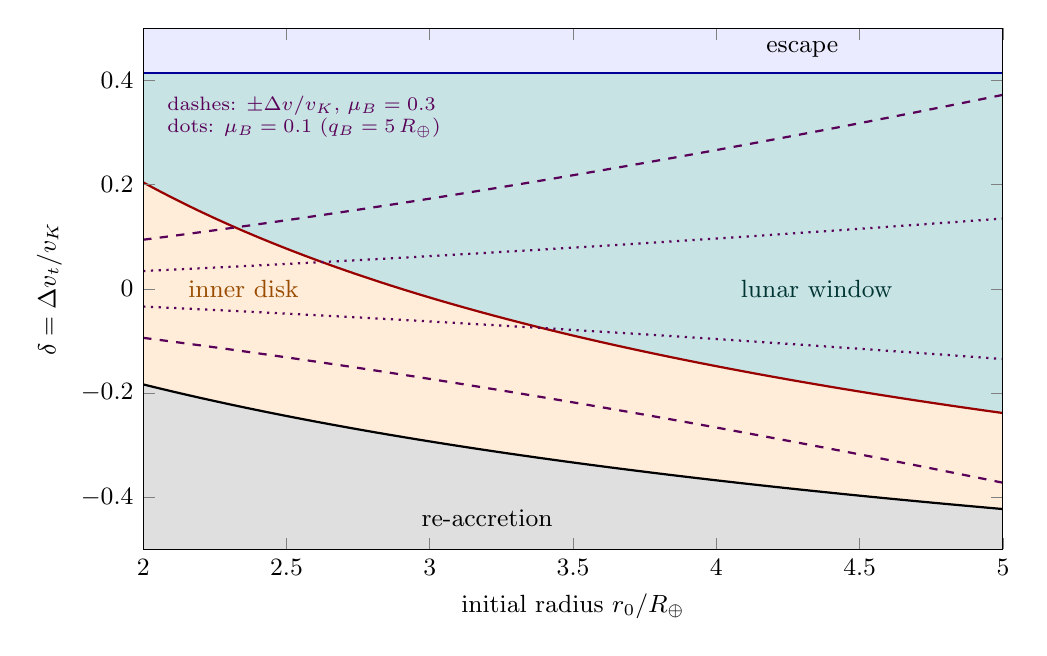
\begin{tikzpicture}
\begin{axis}[width=12.5cm,height=8.2cm,xmin=2,xmax=5,ymin=-0.5,ymax=0.5,
  xlabel={initial radius $r_0/\Rt$},ylabel={$\delta=\Delta v_t/v_K$},
  tick label style={font=\small},label style={font=\small},axis on top]
  \addplot[name path=bas,draw=none,domain=2:5] {-0.5};
  \addplot[name path=haut,draw=none,domain=2:5] {0.5};
  \addplot[name path=re,thick,black,domain=2:5,samples=60] {sqrt(2/(x+1))-1};
  \addplot[name path=L,thick,red!60!black,domain=2:5,samples=60] {sqrt(2.9/x)-1};
  \addplot[name path=esc,thick,blue!60!black,domain=2:5] {0.41421};
  \addplot[gray!25] fill between[of=bas and re];
  \addplot[orange!15] fill between[of=re and L];
  \addplot[teal!22] fill between[of=L and esc];
  \addplot[blue!8] fill between[of=esc and haut];
  \addplot[dashed,thick,violet!70!black,domain=2:5,samples=40] {0.3721*(x/5)^1.5};
  \addplot[dashed,thick,violet!70!black,domain=2:5,samples=40] {-0.3721*(x/5)^1.5};
  \addplot[dotted,thick,violet!70!black,domain=2:5,samples=40] {0.1348*(x/5)^1.5};
  \addplot[dotted,thick,violet!70!black,domain=2:5,samples=40] {-0.1348*(x/5)^1.5};
  \node[font=\small] at (axis cs:4.3,0.46) {escape};
  \node[font=\small,teal!40!black] at (axis cs:4.35,0.0) {lunar window};
  \node[font=\small,orange!60!black] at (axis cs:2.35,0.0) {inner disk};
  \node[font=\small] at (axis cs:3.2,-0.44) {re-accretion};
  \node[font=\scriptsize,violet!70!black,align=left,anchor=west] at (axis cs:2.05,0.33) {dashes: $\pm\Delta v/v_K$, $\mu_B=0.3$\\dots: $\mu_B=0.1$ ($q_B=5\,\Rt$)};
\end{axis}
\end{tikzpicture}
\caption{Analytical map of orbital sorting for a tangential impulse: re-accretion, Roche-interior
disk, lunar window and escape as functions of the initial radius $r_0$ and relative impulse
$\delta$. The violet curves give the order-of-magnitude amplitude of the tidal impulse
\eqref{eq:impulsion} for a passage at $q_B=5\,\Rt$. This is an order-of-magnitude map, replaced in
Phase~B by the exact calculation.}
\label{fig:tri}
\end{figure}

\begin{controle}
Figure~\ref{fig:tri} shows that the lunar window is accessible: for $\mu_B\sim0.3$ and a passage at
$q_B=5\,\Rt$, matter initially near $2.5$--$3\,\Rt$ receives impulses that make it enter the window,
without reaching the escape threshold or the re-accretion threshold. The exact boundaries of this
region are an output of Phase~B.
\end{controle}

\section{From orbital sorting to a dominant satellite}

Orbital sorting also gives a physical explanation for the formation of a dominant satellite. If
$B$ excites a reservoir already containing aggregates or moonlets, it can produce
\begin{equation}
\begin{gathered}
\text{orbital excitation}\rightarrow\text{orbit crossings}\rightarrow
\text{collisions among circumterrestrial bodies}\\
\rightarrow\text{coalescence}\rightarrow f_{\mathrm{dom}}\rightarrow1.
\end{gathered}
\label{eq:chaine-dominance}
\end{equation}
The collisions involve the matter of the reservoir and its aggregates; the Earth--$B$ encounter
remains non-collisional. $N$-body simulations of a circumterrestrial disk indeed show that such a
disk tends to form a single satellite \cite{Kokubo2000}.

\begin{consequence}
In Phase~C simulations, the number of surviving large bodies must decrease after the passage, and
the satellite mass must concentrate into one dominant body: $N_{\mathrm{sat}}\to1$,
$f_{\mathrm{dom}}\to1$.
\end{consequence}

% ---------------------------------------------------------------------
\chapter{Balances of the encounter}
\label{ch:bilans}
% ---------------------------------------------------------------------

The encounter ends when the forcing by $B$ becomes negligible. This chapter closes its mass and
angular-momentum balances in the language of reservoirs: the reservoir mass is distributed
according to partition~\eqref{eq:partition}, and the total angular momentum~\eqref{eq:conservation-J}
is conserved.

\section{Mass balance}

The post-encounter disk verifies
\begin{equation}
M_{D,1}=M_{D,0}+M_{\oplus\to D}+M_{B\to D}-M_{\mathrm{reaccr}}-M_{\mathrm{esc}}-M_{\to B}.
\label{eq:bilanM1}
\end{equation}
It is decomposed by provenance, each term being net of the losses undergone by the corresponding
matter:
\begin{equation}
M_{D,1}=M_{D,1}^{(0)}+M_{D,1}^{(\oplus)}+M_{D,1}^{(B)},
\label{eq:provenance}
\end{equation}
where $M_{D,1}^{(0)}$ is the mass of the preexisting disk retained in the reorganized disk,
$M_{D,1}^{(\oplus)}$ the injected and retained proto-terrestrial mass, and $M_{D,1}^{(B)}$ the mass
possibly ceded by $B$ and retained. This decomposition directly feeds the geochemical fractions of
Chapter~\ref{sec:geochimie}.

\section{Angular-momentum balance}

The balance is written in the barycentric frame of the Earth--$B$ pair, inertial on the encounter
time scale (the solar torque is negligible over $t_{\mathrm{enc}}$). The geocentric frame of
Eq.~\eqref{eq:adiff} is not inertial; it is used for trajectory integration, but not for closing the
balance. Before and after the encounter,
\begin{align}
J_{\mathrm{before}}&=S_{\oplus,0}+S_{B,0}+L_{D,0}+L_{\mathrm{orb},0},
\label{eq:Javant}\\
J_{\mathrm{after}}&=S_{\oplus,1}+S_{B,1}+L_{D,1}+L_{\mathrm{orb},1}+L_{\mathrm{esc}},
\label{eq:Japres}
\end{align}
where $L_{\mathrm{orb}}$ is the orbital angular momentum of the relative Earth--$B$ motion and $S_B$
the spin of $B$, modified by tidal torques. Closure requires
\begin{equation}
\boxed{\;J_{\mathrm{before}}=J_{\mathrm{after}}\;}
\label{eq:fermeture}
\end{equation}
and the Earth--disk system left by the passage is characterized by
\begin{equation}
J_{\oplus D,1}=S_{\oplus,1}+L_{D,1}.
\label{eq:J1}
\end{equation}

\begin{controle}
The angular-momentum transfer toward the trajectory of $B$ is an output of balance closure during
the encounter. The central diagnostic is the Earth--disk state produced after the passage,
$J_{\oplus D,1}$, to be compared with the angular momentum of the Earth--Moon system.
\end{controle}

% =====================================================================

\begin{rappel}
At the end of the encounter, $B$ has ceased to act. The circumterrestrial reservoir has been
sorted: one bound cohort occupies the lunar window, another forms the inner disk, and part has
re-accreted or escaped. The next part follows the evolution of this reservoir, from its supply
before the encounter to lunar accretion.
\end{rappel}

% =====================================================================
\part{The secondary disk as an evolving reservoir}
\label{part:reservoir}
% =====================================================================

\noindent
The secondary disk is not treated here as a fixed object, but as an evolving reservoir $\RD(t)$: it
is fed, transports angular momentum, cools, condenses, forms aggregates, is sorted by the passage
of $B$, then relaxes and accretes the Moon. Its state at each instant combines components of
different nature,
\begin{equation}
\RD(t)=\mathcal{D}_{\mathrm{gas}}(t)\cup\mathcal{D}_{\mathrm{multiphase}}(t)\cup
\mathcal{D}_{\mathrm{particulate}}(t)\cup\mathcal{G}(t),
\label{eq:RD}
\end{equation}
where $\mathcal{G}(t)$ denotes the population of aggregates and moonlets. The three chapters in
this part follow this reservoir before, during and after the passage.

% ---------------------------------------------------------------------
\chapter{Feeding and structure of the reservoir before the passage}
\label{ch:structure}
% ---------------------------------------------------------------------

\section{Accretional origin of the reservoir}
\subsection{Matter supply in the Hill sphere}

The Hill radius of the proto-Earth on its heliocentric orbit is
\begin{equation}
R_H=a_\oplus\left(\frac{\Mt}{3M_\odot}\right)^{1/3}.
\label{eq:RH}
\end{equation}
Matter entering this region may carry non-zero geocentric angular momentum. Pebble accretion
transmits prograde angular momentum \cite{JohansenLacerda2010,Visser2020}, and hydrodynamical
simulations resolve gas and pebble flows around rocky embryos up to one Earth mass
\cite{Popovas2018}. The general physics of accretion disks then links dissipation and
angular-momentum transport \cite{Pringle1981}.

The disk mass balance is
\begin{equation}
\frac{\dd M_D}{\dd t}=\dot M_{\mathrm{in}}-\dot M_{\oplus}-\dot M_{\mathrm{out}},
\label{eq:bilanM}
\end{equation}
where $\dot M_{\mathrm{in}}$ is given by Eq.~\eqref{eq:canaux}, $\dot M_\oplus$ denotes re-accretion
onto the proto-Earth, and $\dot M_{\mathrm{out}}$ losses toward the exterior.

\subsection{Mass and surface density}

The instantaneous disk mass and its ratio to the proto-terrestrial mass are
\begin{equation}
M_D(t)=2\pi\int_{R_{\mathrm{in}}(t)}^{R_{\mathrm{out}}(t)}\Sigma(r,t)\,r\,\dd r,
\qquad
\mu_D(t)=\frac{M_D(t)}{\Mt}.
\label{eq:MD}
\end{equation}

\begin{lecture}
$M_D$ is an output of the feeding and loss balance. The ratio of about $10^{-4}$ obtained for giant
planets in continuously fed models \cite{CanupWard2006} is an astrophysical reference; it does not
fix $\mu_D$ for the proto-Earth, whose feeding mode is different (Section~\ref{sec:soustherm}).
\end{lecture}

\subsection{Angular momentum supplied by accretion}

For a closed control surface $\mathcal{S}_H$ surrounding the terrestrial region of influence, with
outward normal $\mathbf{n}$, the incoming angular-momentum flux is
\begin{equation}
\dot L_{\mathrm{in}}=-\oint_{\mathcal{S}_H}\rho\,(\mathbf{r}\times\mathbf{v})_z\,
(\mathbf{v}\cdot\mathbf{n})\,\dd\mathcal{S},
\label{eq:Lin}
\end{equation}
the minus sign making an incoming contribution positive. The disk angular-momentum balance is
\begin{equation}
\frac{\dd L_D}{\dd t}=\dot L_{\mathrm{in}}-\dot L_{\oplus}-\dot L_{\mathrm{out}}
+\mathcal{T}_{\oplus D}+\mathcal{T}_{\odot D},
\label{eq:bilanL}
\end{equation}
with $\mathcal{T}_{\oplus D}$ and $\mathcal{T}_{\odot D}$ the torques exerted by the proto-Earth and
the Sun.

\subsection{Origin of proto-terrestrial spin}

Pebble accretion can transmit prograde angular momentum to the central body
\cite{JohansenLacerda2010,Visser2020}. The rotation of the proto-Earth therefore belongs to the
same accretion problem as the disk. The reduced rotation is defined as
\begin{equation}
\tilde\omega=\frac{\Omega_\oplus}{\sqrt{G\Mt/\Req^3}}.
\label{eq:omegatilde}
\end{equation}
For an approximately spin-conserving contraction,
\begin{equation}
S_\oplus\simeq k\,\Mt\Req^2\Omega_\oplus\simeq\text{constant}
\quad\Longrightarrow\quad
\tilde\omega\propto\Req^{-1/2}
\label{eq:spin}
\end{equation}
when $k$ and $\Mt$ vary little: thermal contraction of a hot proto-Earth brings it closer to
critical rotation.

\begin{ideephys}
The disk and Earth's spin are not two independent reservoirs added together. Both result from how
matter and angular momentum are distributed during the growth of the proto-Earth; the channel
$\dot M_{\mathrm{rot}}$ directly links them.
\end{ideephys}

% =====================================================================

\section{Radial structure}
\subsection{Inner radius}

The inner radius corresponds to the transition between the proto-Earth or its dense envelope and a
truly orbital regime:
\begin{equation}
R_{\mathrm{in}}\simeq R_{\mathrm{tr}}.
\label{eq:Rin}
\end{equation}
This transition depends on pressure, rotation, temperature and, if a significant magnetic field is
present, on magnetohydrodynamic constraints. For a proto-Earth close to critical rotation,
$R_{\mathrm{tr}}$ tends toward $\Req$.

\subsection{Outer radius}

The outer radius is parameterized by
\begin{equation}
R_{\mathrm{out}}=\xi_H R_H,\qquad 0<\xi_H<1.
\label{eq:Rout}
\end{equation}
For circumplanetary disks of giant planets, truncation by solar torques leads to
$\xi_H\approx0.3$--$0.4$ \cite{QuillenTrilling1998,MartinLubow2011}; in the present theory,
$\xi_H$ is an output of heliocentric dynamics and feeding conditions. The bulk of the mass of a
solid-fed disk nevertheless concentrates well inside this edge, near the circularization radius of
captured matter.

\subsection{Roche limit and synchronous orbit}

For a reference satellite density $\rho_s$, the fluid Roche limit is
\begin{equation}
\aR\simeq2.456\left(\frac{3\Mt}{4\pi\rho_s}\right)^{1/3}
\approx2.9\,\Rt\quad(\rho_s=3.34\ \mathrm{g\,cm^{-3}}).
\label{eq:Roche}
\end{equation}
Its role is distinct from that of $R_{\mathrm{in}}$:
\begin{equation}
R_{\mathrm{in}}\neq\aR.
\label{eq:RinRoche}
\end{equation}
A second radius plays an essential dynamical role, the synchronous orbit
\begin{equation}
a_{\mathrm{sync}}=\left(\frac{G\Mt}{\Omega_\oplus^2}\right)^{1/3}\approx2.0\text{--}2.3\,\Rt
\quad(P_\oplus=4\text{--}5\ \mathrm{h}).
\label{eq:async}
\end{equation}
For a rapidly rotating proto-Earth, $a_{\mathrm{sync}}<\aR$: any body assembled beyond the Roche
limit migrates outward under the effect of terrestrial tides.

\begin{lecture}
A disk can occupy the region interior to the Roche limit. This limit controls the survival and
assembly of large self-gravitating aggregates; it is central to lunar accretion, not to the
existence of the disk. The ordering $a_{\mathrm{sync}}<\aR$ ensures that bodies formed beyond Roche
move away from Earth rather than fall back onto it.
\end{lecture}

\begin{figure}[htbp]
\centering
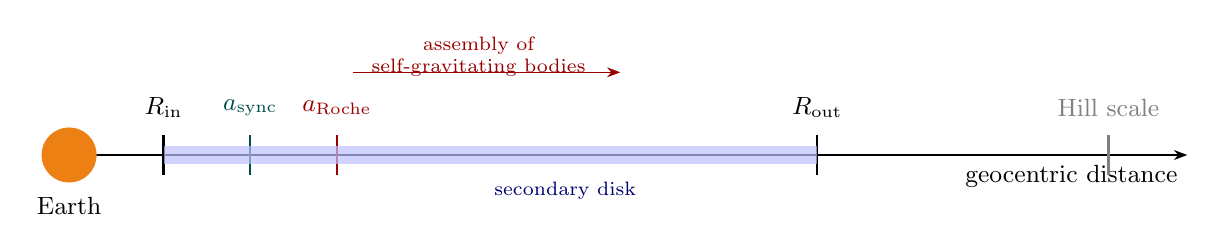
\begin{tikzpicture}
  \draw[-{Stealth}] (0,0) -- (14.2,0) node[below left,font=\small] {geocentric distance};
  \fill[orange!70!brown] (0,0) circle (0.35);
  \node[font=\small] at (0,-0.65) {Earth};
  \foreach \x/\lab/\c in {1.2/{$R_{\mathrm{in}}$}/black,2.3/{$a_{\mathrm{sync}}$}/teal!60!black,3.4/{$\aR$}/red!60!black,9.5/{$R_{\mathrm{out}}$}/black,13.2/{Hill scale}/gray}{
    \draw[\c,thick] (\x,-0.25) -- (\x,0.25);
    \node[\c,font=\small] at (\x,0.6) {\lab};
  }
  \fill[blue!25,opacity=0.7] (1.2,-0.12) rectangle (9.5,0.12);
  \node[font=\scriptsize,blue!45!black] at (6.3,-0.45) {secondary disk};
  \node[font=\scriptsize,red!60!black,align=center] at (5.2,1.25) {assembly of\\self-gravitating bodies};
  \draw[red!60!black,-{Stealth}] (3.6,1.05) -- (7.0,1.05);
\end{tikzpicture}
\caption{Conceptual radial organization of the circumterrestrial disk. The inner, synchronous,
Roche, outer and Hill radii play different physical roles (not to scale).}
\label{fig:radial}
\end{figure}

% =====================================================================

\section{Orbital structure and angular-momentum transport}
\subsection{Quasi-Keplerian rotation}

When the disk mass remains small compared with that of the proto-Earth and pressure provides only
a moderate correction, the dominant orbital frequency is
\begin{equation}
\Omega_K(r)=\sqrt{\frac{G\Mt}{r^3}}.
\label{eq:OmegaK}
\end{equation}
The actual azimuthal velocity is
\begin{equation}
v_\phi^2=\frac{G\Mt}{r}+\frac{r}{\rho}\frac{\partial P}{\partial r}+r\,a_{\mathrm{sg}}(r)
+r\,a_{J_2}(r),
\label{eq:vphi}
\end{equation}
where $a_{\mathrm{sg}}$ represents the disk self-gravity and $a_{J_2}$ the contribution of the
flattening of a rapidly rotating proto-Earth. The specific angular momentum is $j(r)=r\,v_\phi(r)$.

\subsection{Global disk angular momentum}

In the Keplerian limit,
\begin{equation}
L_D=2\pi\int_{R_{\mathrm{in}}}^{R_{\mathrm{out}}}\Sigma(r)\sqrt{G\Mt r}\;r\,\dd r,
\label{eq:LD}
\end{equation}
and the initial Earth--disk system has
\begin{equation}
J_{\oplus D,0}=S_{\oplus,0}+L_{D,0}.
\label{eq:J0}
\end{equation}

\begin{ideephys}
The angular momentum destined for the future Moon may already be partly orbital before the passage
of $B$. The encounter therefore does not have to create the entire orbital budget: it redistributes
a budget already present and adds or removes the part exchanged with the trajectory of $B$.
\end{ideephys}

\subsection{Viscous evolution}

In the approximation of a thin, axisymmetric, quasi-Keplerian disk, the surface density follows the
classical equation \cite{Pringle1981}
\begin{equation}
\frac{\partial\Sigma}{\partial t}=\frac{3}{r}\frac{\partial}{\partial r}
\left[r^{1/2}\frac{\partial}{\partial r}\left(\nu\Sigma r^{1/2}\right)\right].
\label{eq:visc}
\end{equation}
For a gaseous component, $\nu=\alpha c_sH$ with $H\simeq c_s/\Omega_K$. For a dense particulate
component, the effective viscosity is dominated by self-gravity wakes and scales as
$G^2\Sigma^2/\Omega_K^3$ \cite{Daisaka2001}. The characteristic viscous time is
\begin{equation}
t_\nu(r)\sim\frac{r^2}{\nu}.
\label{eq:tnu}
\end{equation}

% ---------------------------------------------------------------------
\chapter{Thermodynamics, stability and persistence}
\label{ch:thermo}
% ---------------------------------------------------------------------

\section{Thermal and multiphase state}
\subsection{Energy balance}

The local energy balance of the disk is
\begin{equation}
Q^{+}_{\mathrm{visc}}+Q^{+}_{\mathrm{acc}}+Q^{+}_{\oplus}+Q^{+}_{\odot}
=Q^{-}_{\mathrm{rad}}+Q^{-}_{\mathrm{adv}}+Q^{-}_{\mathrm{phase}}.
\label{eq:bilanE}
\end{equation}
In a quasi-Keplerian disk, viscous dissipation per unit surface and radiative cooling from both
faces are
\begin{equation}
Q^{+}_{\mathrm{visc}}\simeq\frac94\,\nu\Sigma\Omega_K^2,
\qquad
Q^{-}_{\mathrm{rad}}\simeq2\sigma_{\mathrm{SB}}T_{\mathrm{eff}}^4.
\label{eq:Qvisc}
\end{equation}
With vertical optical depth $\tau\simeq\kappa\Sigma/2$, the diffusion approximation gives, for an
optically thick medium,
\begin{equation}
T_{\mathrm{mid}}^4\simeq\frac34\,\tau\,T_{\mathrm{eff}}^4+T_{\mathrm{irr}}^4.
\label{eq:Tmid}
\end{equation}

\begin{lecture}
Temperature enters simultaneously into thickness, viscosity, opacity, sound speed and phase state.
Thermodynamics directly participates in the orbital structure and lifetime of the disk; it is not a
module added after the dynamics.
\end{lecture}

\subsection{Condensation and phase transitions}

For each species $i$, the phase state is a function
\begin{equation}
\mathcal{P}_i=\mathcal{P}_i\!\left[T(r,t),\,P(r,t),\,f_{\mathrm{O_2}}(r,t),\,\mathbf{X}(r,t)\right],
\label{eq:phase}
\end{equation}
and the solid-evolution chain is
\begin{equation}
\text{vapor}\rightarrow\text{condensates}\rightarrow\text{grains}\rightarrow
\text{aggregates}\rightarrow\text{satellitesimals}.
\label{eq:chaine}
\end{equation}
For a population of particles with number density $n_p$, collision cross-section $\sigma_c$ and
relative velocity $\Delta v$, the collision time has the scale
\begin{equation}
t_{\mathrm{coll}}\sim\frac{1}{n_p\,\sigma_c\,\Delta v}.
\label{eq:tcoll}
\end{equation}

\subsection{Vertical settling}

A particle coupled to the gas is characterized by its Stokes number
$\mathrm{St}=t_{\mathrm{stop}}\Omega_K$. The competition between settling and turbulence fixes its
vertical thickness:
\begin{equation}
\frac{H_p}{H}\sim\left(\frac{\alpha}{\alpha+\mathrm{St}}\right)^{1/2}.
\label{eq:Hp}
\end{equation}
This relation follows the emergence of a solid-enriched midplane.

% =====================================================================

\section{Gravitational stability and persistence}
\subsection{Toomre criterion}

The local stability of a self-gravitating thin disk is measured by the Toomre parameter, whose
constant depends on the nature of the medium:
\begin{equation}
Q_T^{\mathrm{gas}}=\frac{c_s\,\kappa_{\mathrm{epi}}}{\pi G\Sigma}
\quad\text{\cite{Safronov1960,GoldreichLyndenBell1965}},
\qquad
Q_T^{\mathrm{part}}=\frac{\sigma_r\,\kappa_{\mathrm{epi}}}{3.36\,G\Sigma}
\quad\text{\cite{Toomre1964}},
\label{eq:Toomre}
\end{equation}
where $\kappa_{\mathrm{epi}}$ is the epicyclic frequency and $\sigma_r$ the radial velocity
dispersion of the particles. A cold and dense disk approaches the regime $Q_T\sim1$.

\begin{ideephys}
The preexistence of the disk raises a decisive question: when $B$ arrives, is the disk still a
diffuse reservoir, or has it already formed aggregates and moonlets? The answer can be calculated
from thermodynamics, gravitational stability and growth times.
\end{ideephys}

\subsection{Disk persistence}

Persistence is expressed through the state of the reservoir at $t_B$ rather than through an
arbitrary duration:
\begin{equation}
M_D(t_B)+\sum_k m_k(t_B)\ \ge\ M_{D,\min},\qquad
L_D(t_B)+\sum_k L_k(t_B)\ \ge\ L_{D,\min},\qquad
R_{\mathrm{out}}(t_B)>R_{\mathrm{in}}(t_B).
\label{eq:persistance}
\end{equation}

\begin{falsif}
If feeding, cooling and transport laws systematically dissipate or re-accrete the reservoir before
any time window compatible with the passage of $B$, the corresponding branch of the theory is
excluded.
\end{falsif}

% =====================================================================

The three chronological regimes describing the state of the reservoir at the time of the passage
were presented in Chapter~\ref{ch:chronologie} (Section~\ref{sec:regimes}).

% ---------------------------------------------------------------------
\chapter{Reservoir reorganization and lunar accretion}
\label{ch:reorganisation}
% ---------------------------------------------------------------------

After orbital sorting, the reservoir enters a phase of dissipative relaxation, then accretion. This
chapter describes the new state of the reservoir, its dissipation, the mass available beyond Roche,
and the control of the accessible satellite mass.

\section{New state of the disk}

The passage provides
\begin{equation}
\mathcal{D}_1=\left\{M_{D,1},\ \Sigma_1,\ T_1,\ \mathbf{X}_1,\ L_{D,1},\ e(r),\ i(r),\
\mathbf{f}_{\mathrm{phase},1},\ \mathcal{G}_1\right\},
\label{eq:D1}
\end{equation}
and the collective evolution follows
\begin{equation}
\mathcal{D}_1\longrightarrow\mathcal{D}_{\mathrm{relax}}\longrightarrow\mathcal{D}_{\mathrm{accr}}
\longrightarrow\text{proto-Moon}.
\label{eq:evolution}
\end{equation}

\section{Dissipation}

The relaxation energy balance is
\begin{equation}
E_{\mathrm{diss}}=E_{\mathrm{shock}}+E_{\mathrm{circ}}+E_{\mathrm{vis}}+E_{\mathrm{coll}}
-E_{\mathrm{rad}}-E_{\mathrm{esc}}.
\label{eq:Ediss}
\end{equation}
A parcel on an orbit with semi-major axis $a$ and eccentricity $e$, circularized at conserved
angular momentum, reaches the radius $a_{\mathrm{circ}}=a(1-e^2)$. The specific energy released,
positive, is
\begin{equation}
\Delta\varepsilon_{\mathrm{circ}}=\frac{G\Mt}{2a_{\mathrm{circ}}}-\frac{G\Mt}{2a}
=\frac{G\Mt}{2a}\,\frac{e^2}{1-e^2}\ \ge0.
\label{eq:circ}
\end{equation}

\section{Mass available beyond Roche}

The mass and angular momentum located beyond the Roche limit are
\begin{equation}
M_{>R}=2\pi\int_{\aR}^{R_{\mathrm{out}}}\Sigma(r)\,r\,\dd r,
\qquad
L_{>R}=2\pi\int_{\aR}^{R_{\mathrm{out}}}\Sigma(r)\sqrt{G\Mt r}\;r\,\dd r.
\label{eq:MR}
\end{equation}

\section{Ida, Canup and Stewart control}

Once the reorganized disk is established, the normalized specific angular momentum is defined as
\begin{equation}
\ell_D=\frac{L_D}{M_D\sqrt{G\Mt\aR}}.
\label{eq:lD}
\end{equation}
The reference relation of Ida, Canup and Stewart \cite{Ida1997,Canup2004} is
\begin{equation}
\frac{M_{L,\mathrm{Ida}}}{M_D}\simeq1.9\,\ell_D-1.1-1.9\,\frac{M_{\mathrm{esc}}}{M_D}.
\label{eq:Ida}
\end{equation}
This relation, calibrated on particulate disks in which the Moon forms near $1.3\,\aR$, is used as
a first-order estimator. When the disk includes a Roche-interior fluid component, the Moon forms
farther away, near $2.15\,\aR$, and the revised estimate of Salmon and Canup \cite{SalmonCanup2012}
must be used. The computed value is bounded to the physical interval
$0\le M_{L,\mathrm{Ida}}\le M_D$.

\begin{lecture}
The Ida relation intervenes after definition of the post-encounter disk. It does not replace
hydrodynamics; it gives a rapid control on the mass scale accessible from the pair $(M_D,L_D)$
produced by the passage of $B$.
\end{lecture}

\begin{figure}[htbp]
\centering
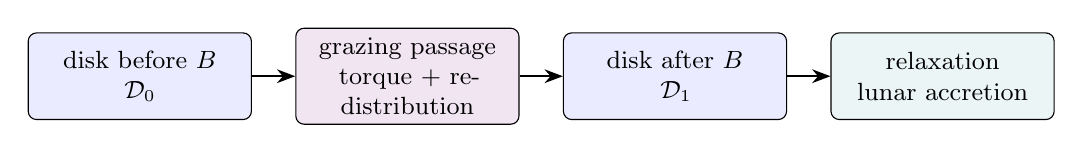
\begin{tikzpicture}[node distance=0.55cm,
  bx/.style={draw,rounded corners=3pt,align=center,font=\small,minimum height=1.1cm,text width=2.6cm,fill=#1},
  bx/.default=white]
  \node[bx=blue!8] (a) {disk before $B$\\$\mathcal{D}_0$};
  \node[bx=violet!10,right=of a] (b) {grazing passage\\torque + redistribution};
  \node[bx=blue!8,right=of b] (c) {disk after $B$\\$\mathcal{D}_1$};
  \node[bx=teal!8,right=of c] (d) {relaxation\\lunar accretion};
  \draw[-{Stealth},thick] (a) -- (b);
  \draw[-{Stealth},thick] (b) -- (c);
  \draw[-{Stealth},thick] (c) -- (d);
\end{tikzpicture}
\caption{The passage of $B$ transforms an existing disk; lunar accretion then acts on the
reorganized disk.}
\label{fig:flux}
\end{figure}

% =====================================================================

\begin{rappel}
The dynamical path is now complete: feeding, orbital sorting, relaxation and accretion. The next
part verifies that it is also a \emph{material} path: the Moon must preserve the chemical memory of
the reservoirs from which it came.
\end{rappel}

% =====================================================================
\part{Geochemistry: families of tracers}
\label{part:geochimie}
% =====================================================================

\noindent
Geochemistry belongs to the same story as dynamics. Each matter element preserves, throughout the
path, its dynamical, thermal and chemical labels. This part first sets the framework of the three
material lineages, then organizes tests by tracer families, each of which answers a precise
physical question.

% ---------------------------------------------------------------------
\chapter{Three material lineages}
\label{sec:geochimie}
% ---------------------------------------------------------------------

\section{Fractions of provenance}

Lunar matter may contain three contributions:
\begin{equation}
f_0+f_\oplus+f_B=1,
\label{eq:fractions}
\end{equation}
where $f_0$ is the fraction inherited from the preexisting disk, $f_\oplus$ the fraction injected
from the proto-Earth during the encounter, and $f_B$ the possible contribution from $B$. The
corresponding masses are
\begin{equation}
M_L^{(k)}=f_k\,M_L,\qquad k\in\{0,\oplus,B\},
\label{eq:MLk}
\end{equation}
and the $f_k$ follow from decomposition~\eqref{eq:provenance}, weighted by the accretion efficiency
of each lineage.

\section{Concentration-weighted isotopic mixing}

For an isotopic system or ratio $R_X$, mixing is weighted by concentrations:
\begin{equation}
R_X^L=\frac{f_0C_{X,0}R_{X,0}+f_\oplus C_{X,\oplus}R_{X,\oplus}+f_BC_{X,B}R_{X,B}}
{f_0C_{X,0}+f_\oplus C_{X,\oplus}+f_BC_{X,B}}.
\label{eq:melange}
\end{equation}
This relation applies separately to the O, Ti, Cr, Si and W systems, each with its own
concentrations.

\begin{ideephys}
The preexisting disk has its own chemical history; its composition cannot be made invisible by
definition. The theory draws a prediction from this: lunar chemistry results from a mixture whose
fractions are computed by dynamics.
\end{ideephys}

\section{One physical question per tracer family}

Geochemical tracers are not interchangeable: each records a different process. The theory groups
them into four families (Figure~\ref{fig:familles}).

\begin{figure}[htbp]
\centering
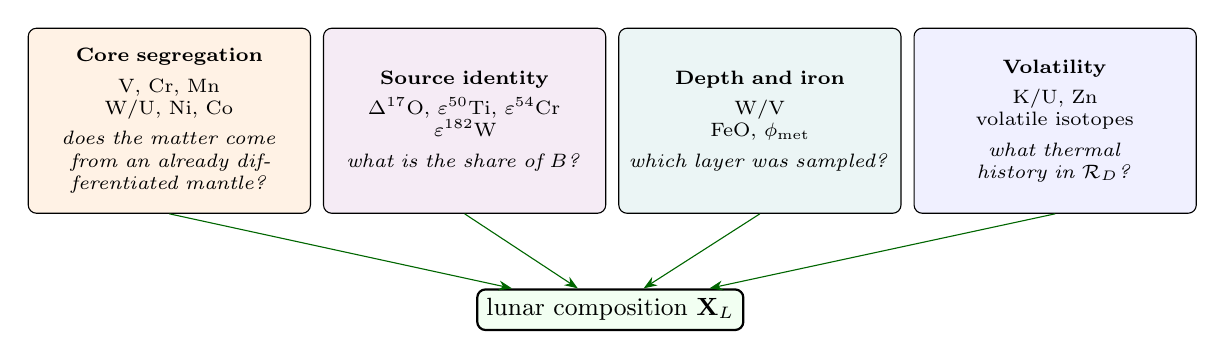
\begin{tikzpicture}[
  fam/.style={draw,rounded corners=3pt,align=center,font=\scriptsize,text width=3.35cm,
              minimum height=2.35cm,fill=#1},fam/.default=white]
  \node[fam=orange!10] (a) at (0,0) {\textbf{Core segregation}\\[3pt]V, Cr, Mn\\W/U, Ni, Co\\[3pt]\emph{does the matter come from an already differentiated mantle?}};
  \node[fam=violet!8] (b) at (3.75,0) {\textbf{Source identity}\\[3pt]$\Delta^{17}$O, $\varepsilon^{50}$Ti, $\varepsilon^{54}$Cr\\$\varepsilon^{182}$W\\[3pt]\emph{what is the share of $B$?}};
  \node[fam=teal!8] (c) at (7.5,0) {\textbf{Depth and iron}\\[3pt]W/V\\FeO, $\phi_{\mathrm{met}}$\\[3pt]\emph{which layer was sampled?}};
  \node[fam=blue!6] (d) at (11.25,0) {\textbf{Volatility}\\[3pt]K/U, Zn\\volatile isotopes\\[3pt]\emph{what thermal history in $\RD$?}};
  \node[draw,thick,rounded corners=3pt,font=\small,fill=green!5] (L) at (5.6,-2.4) {lunar composition $\mathbf{X}_L$};
  \foreach \n in {a,b,c,d} \draw[-{Stealth},green!40!black] (\n.south) -- (L);
\end{tikzpicture}
\caption{The four tracer families and the physical question answered by each.}
\label{fig:familles}
\end{figure}

% ---------------------------------------------------------------------
\chapter{Families of tracers}
\label{ch:traceurs}
% ---------------------------------------------------------------------

\section{Moderately siderophile refractory elements: V, Cr, Mn}

Chromium, vanadium and manganese have similar abundances in Earth's mantle and in the Moon, and
they are clearly depleted relative to their primitive abundances normalized to magnesium
\cite{Ringwood1990}. This similarity has been used to suggest that the Moon derives substantially
from Earth's mantle after core formation \cite{Drake1989}.

Vanadium has a particular place in this family. It is less volatile than magnesium: its depletion
cannot result from evaporative loss, either in the nebula or in the circumterrestrial reservoir. It
records metal--silicate segregation.

The debate must be reported faithfully. Experiments at 1~bar showed that the depletions of V, Cr
and Mn do not follow metal/silicate partition coefficients measured under those conditions, which
led to the conclusion that they were not primarily explained by terrestrial core formation
\cite{Drake1989}. High-pressure experiments subsequently showed that, under lower-mantle
conditions, the behavior of these elements changes with the increasing solubility of oxygen in
liquid iron, so that similar depletion patterns in Earth and Moon indicate that a large fraction of
the Moon comes from Earth's mantle after core segregation \cite{Ringwood1990,GessmannRubie2000}.

\begin{lecture}
A small Moon at low internal pressure hardly produces by itself a vanadium depletion characteristic
of high-pressure segregation. In the present theory, this signature is interpreted as the trace of
a flux of terrestrial silicate matter toward the reservoir, $\Phi_{\oplus\to D}$. Vanadium is not
read in isolation: it is interpreted together with tungsten and the other tracers of the same
lineage.
\end{lecture}

\section{Tungsten: abundance, isotopes and clock}

Tungsten provides two independent pieces of information.

\paragraph{Its abundance.}
The W/U, or W/Th, ratio compares elements of similar incompatibility during silicate melting. It is
therefore only weakly sensitive to magmatic differentiation and records the siderophile behavior of
tungsten, that is, metal segregation \cite{Newsom1986}. A lunar value close to the terrestrial
value indicates a silicate source that underwent the same segregation history.

\paragraph{Its isotopes.}
After correction for late accretion, lunar $\varepsilon^{182}$W is almost identical to that of
Earth's mantle \cite{Kruijer2015,Touboul2015}. In a collision scenario, this identity requires a
specific explanation because the mantle of the impactor would have carried its own signature. In
the present theory, it corresponds to what is expected, since lunar tungsten comes mainly from
terrestrial silicate matter; this expectation must be checked in the viable domain.

\paragraph{A clock.}
If the sampled layer had acquired an Hf/W ratio different from that of the mean mantle, decay of
$^{182}$Hf (half-life 8.9~Ma) would have produced an excess or deficit of $^{182}$W, unless
$^{182}$Hf was already extinct. Tungsten therefore constrains both the source and the time $t_B$.

\paragraph{Bound on reservoir composition.}
With $f_B=0$ and the silicate Earth as reference ($\varepsilon^{182}\mathrm{W}_\oplus=0$), the
linearized form of Eq.~\eqref{eq:melange} gives (Appendix~\ref{app:borneW})
\begin{equation}
\varepsilon^{182}\mathrm{W}_L\simeq f_0\,\frac{C_{\mathrm{W},0}}{C_{\mathrm{W},\oplus}}\,
\varepsilon^{182}\mathrm{W}_0
\quad\Longrightarrow\quad
f_0\lesssim\frac{\delta\varepsilon\;C_{\mathrm{W},\oplus}}{C_{\mathrm{W},0}\,|\varepsilon^{182}\mathrm{W}_0|},
\label{eq:bornef0}
\end{equation}
where $\delta\varepsilon$ is the tolerated Earth--Moon difference; this bound applies if the
reservoir material is chondritic. With $C_{\mathrm{W},0}\approx0.1$--$0.2$~ppm,
$\varepsilon^{182}\mathrm{W}_0\approx-1.9$, $C_{\mathrm{W},\oplus}\approx0.013$~ppm and
$\delta\varepsilon\approx0.1$--$0.2$, chondritic matter could represent only $0.3$ to $1.4\,\%$ of
the Moon.

\begin{lecture}
Because the theory assigns the principal share of lunar matter to the preexisting reservoir,
bound~\eqref{eq:bornef0} requires this reservoir to be of \emph{terrestrial silicate} nature:
$\varepsilon^{182}\mathrm{W}_0\simeq0$, and the bound disappears. This points to equatorial mass loss
$\Phi^{\mathrm{rot}}_{\oplus\to D}$ and ordinary mantle-impact ejecta as the dominant supply of
$\RD$, with co-accretion of chondritic matter remaining minor. This is a prediction of the theory:
the composition of the circumterrestrial reservoir is terrestrial.
\end{lecture}

\section{Iron and siderophiles: FeO, Ni, Co and metal}

Most refractory lithophile and weakly siderophile elements have similar abundances in the Moon and
silicate Earth, but FeO appears significantly higher in the lunar mantle, which is an important
constraint on origin models \cite{Canup2023}. The framework of three lineages makes it possible to
treat this quantitatively.

\subsection{FeO and silicate reservoir}

For a simplified mixture, the FeO content of the disk after the encounter is
\begin{equation}
X^{D,1}_{\mathrm{FeO}}=f_0X^{0}_{\mathrm{FeO}}+f_\oplus X^{\oplus}_{\mathrm{FeO}}+f_BX^{B}_{\mathrm{FeO}},
\label{eq:FeO}
\end{equation}
then corrected for fractionations due to melting, condensation and vapor loss. If a melt fraction
$F$ is extracted from a reservoir with a bulk partition coefficient $D_X$, a fractional-melting law
for example gives
\begin{equation}
C_X^{\mathrm{liq}}=C_{X,0}\,\frac{1-(1-F)^{1/D_X}}{F}.
\label{eq:fusion}
\end{equation}
The calculation does not choose one depth for FeO, another for W and a third for isotopes: the same
material lineage carries all properties.

\subsection{Metal and silicate}

The disk is decomposed into
\begin{equation}
M_D=M_D^{\mathrm{sil}}+M_D^{\mathrm{met}}+M_D^{\mathrm{vap}},
\qquad
\phi_{\mathrm{met}}=\frac{M_D^{\mathrm{met}}}{M_D^{\mathrm{sil}}+M_D^{\mathrm{met}}}.
\label{eq:metal}
\end{equation}
The siderophile elements Ni, Co and W constrain the origin, segregation and re-accretion of metal.

\begin{consequence}
The lunar FeO excess must be reproduced by the calculation of mixing and internal transformations
within the reservoir ($\boldsymbol{\Pi}_D$ in Eq.~\eqref{eq:flux-X}): oxidation of part of the metal,
fractionation during condensation, or a more oxidized silicate component. Because
bound~\eqref{eq:bornef0} limits the chondritic share, the excess must come from internal reservoir
processes.
\end{consequence}

\section{O, Ti, Cr isotopes: the imprint of \texorpdfstring{$B$}{B}}
\label{sec:bornes}

The oxygen, titanium and chromium isotopic systems distinguish Solar System bodies according to
their formation reservoir. They therefore measure the share of $B$ in the Moon. For oxygen, at
comparable concentrations,
\begin{equation}
f_B\lesssim\frac{\delta_{17}}{|\Delta^{17}\mathrm{O}_B-\Delta^{17}\mathrm{O}_\oplus|},
\label{eq:bornefB}
\end{equation}
where $\delta_{17}$, of order a few ppm, is the measured Earth--Moon difference \cite{Young2016}.
For a body $B$ with Martian-like isotopic composition
($|\Delta^{17}\mathrm{O}_B-\Delta^{17}\mathrm{O}_\oplus|\approx300$~ppm), $f_B\lesssim2\,\%$.
Titanium \cite{Zhang2012} and chromium constraints are expressed in the same way.

\begin{apport}
The mechanism naturally favors a small material contribution from $B$, because the passage is
non-collisional. The Earth--Moon isotopic similarity therefore becomes an expected constraint of
the viable domain, to be checked through the bounds on $f_B$ (Eq.~\eqref{eq:bornefB}).
\end{apport}

\section{Volatiles}

For a volatile species $i$, the balance and isotopic fractionation associated with vapor loss of
Rayleigh type are
\begin{equation}
\frac{\dd M_i}{\dd t}=\dot M_{i,\mathrm{in}}-\dot M_{i,\oplus}-\dot M_{i,\mathrm{esc}}
+\dot M_{i,\mathrm{cond}}-\dot M_{i,\mathrm{vap}},
\qquad
R_i=R_{i,0}\,f_i^{(\alpha_i-1)},
\label{eq:volatils}
\end{equation}
where $f_i$ is the residual fraction and $\alpha_i$ the effective fractionation factor.

\section{The W/V ratio and depth of origin}

Tungsten and vanadium are not isolated proofs: they are \emph{coupled tracers} of fluxes between
reservoirs and of the depth of the sampled matter. Their interpretation passes through the
composition equation~\eqref{eq:flux-X} and the injected-matter distribution~\eqref{eq:flux}.

Tungsten is highly incompatible: during crystallization of a magma ocean, it concentrates in the
last liquids and therefore toward the surface. Vanadium is moderately compatible, retained by
pyroxenes and spinels. The W/V ratio, normalized to reference elements with similar behavior,
therefore varies with the depth and differentiation state of the sampled layer. For injected matter
it is
\begin{equation}
\left(\frac{\mathrm{W}}{\mathrm{V}}\right)_{\oplus\to D}=
\frac{\displaystyle\iiint\frac{\dd M_{\oplus\to D}}{\dd\lambda_\Omega\,\dd z\,\dd t}\,
C_{\mathrm{W}}(\lambda_\Omega,z)\,\dd\lambda_\Omega\,\dd z\,\dd t}
{\displaystyle\iiint\frac{\dd M_{\oplus\to D}}{\dd\lambda_\Omega\,\dd z\,\dd t}\,
C_{\mathrm{V}}(\lambda_\Omega,z)\,\dd\lambda_\Omega\,\dd z\,\dd t}.
\label{eq:WV}
\end{equation}

\begin{ideephys}
This is the most direct expression of the single material lineage: the same depth distribution $z$
and latitude distribution $\lambda_\Omega$, produced by the passage dynamics (Eq.~\eqref{eq:flux}),
simultaneously fix the injected mass and its elemental ratios. One does not choose a separate depth
for each tracer.
\end{ideephys}

\section{Synthesis of tracers}

\begin{table}[htbp]
\centering
\small
\caption{Tracer families, recorded processes and predictions of the theory.}
\label{tab:traceurs}
\begin{tabularx}{\textwidth}{>{\raggedright\arraybackslash}p{2.6cm}
>{\raggedright\arraybackslash}X >{\raggedright\arraybackslash}X}
\toprule
\textbf{Tracer} & \textbf{What it records} & \textbf{Prediction of the theory} \\
\midrule
V, Cr, Mn & high-pressure core segregation & lunar depletions similar to terrestrial ones \\
W/U, W/Th & siderophile behavior of tungsten & lunar ratio close to the terrestrial ratio \\
$\varepsilon^{182}$W & source identity, chronology & close to Earth's mantle; constraint on $t_B$ \\
$\Delta^{17}$O, $\varepsilon^{50}$Ti, $\varepsilon^{54}$Cr & share of $B$ & $f_B\ll1$ \\
FeO, $\phi_{\mathrm{met}}$ & oxidized iron and metal & lunar excess produced in the reservoir \\
W/V & depth and differentiation of the sampled layer & linked to stripped latitude and depth \\
K/U, Zn & thermal history of the reservoir & depletion produced in $\RD$ \\
\bottomrule
\end{tabularx}
\end{table}

\begin{rappel}
Dynamics and geochemistry now describe the same path. The next part gathers the conditions that it
must satisfy simultaneously: the viability domain.
\end{rappel}

% =====================================================================
\part{Viability domain}
\label{part:viabilite}
% =====================================================================

\noindent
A physical path is credible only if it exists within a continuous region of parameter space, not
for a single finely tuned configuration. This part gathers the Level~I parameters, the gates that
the path must pass simultaneously, and the numerical program that will produce the viability maps.

% ---------------------------------------------------------------------
\chapter{Parameters, gates and viable domain}
\label{ch:portes}
% ---------------------------------------------------------------------

\section{Level I parameters}

The vector $\Theta_I$ (Eq.~\eqref{eq:Theta}) groups the parameters of the proto-Earth, the
reservoir and the encounter. Table~\ref{tab:grille} proposes an initial exploration grid; the
prograde low-latitude band is designated as the priority region.

\begin{table}[htbp]
\centering
\small
\caption{Initial exploration grid for Level I parameters.}
\label{tab:grille}
\begin{tabular}{lll}
\toprule
\textbf{Parameter} & \textbf{Initial domain} & \textbf{Comment} \\
\midrule
$\mu_B=M_B/\Mt$ & $0.05$--$1$ & mass of $B$ \\
$q_B$ & $2.75$--$10\,\Rt$ & lower bound: caution threshold (static tide) \\
$v_\infty$ & $0$--$10$ km\,s$^{-1}$ & relative asymptotic velocity \\
$t_{\mathrm{ej}}$ & $>t_B$ & later elimination or ejection of $B$ \\
$i_B$ & $0$--$180^\circ$ & priority: $|\lambda_B|\le\lambda_c$, prograde \\
$\omega_B$ & $0$--$180^\circ$ & priority: near $90^\circ$ \\
$\tilde\omega$ & $0.8$--$1$ & reduced proto-Earth rotation \\
$\Req/\Rt$ & $1$--$1.3$ & flattening \\
Reservoir & $2$--$5\,\Rt$, $\Sigma\propto r^{-p}$, $p\in[0,3]$ & radial structure \\
$M_{D,0}$ & of order a few $M_L$ & initial reservoir mass \\
\bottomrule
\end{tabular}
\end{table}

\section{Gates of the viable domain}

The total domain is defined by the intersection
\begin{equation}
\boxed{\begin{aligned}
\mathcal{D}_{\mathrm{viable}}=\ &\mathcal{D}_{\mathrm{disk},0}\cap\mathcal{D}_{\mathrm{thermo}}
\cap\mathcal{D}_{\mathrm{grav}}\cap\mathcal{D}_{\mathrm{nc}}\cap\mathcal{D}_{\mathrm{nt}}
\cap\mathcal{D}_{B}\cap\mathcal{D}_{B,\mathrm{hel}}\\
&\cap\mathcal{D}_{\mathrm{fen}}\cap\mathcal{D}_{J}\cap\mathcal{D}_{\mathrm{accr}}\cap\mathcal{D}_{\mathrm{arch}}
\cap\mathcal{D}_{\mathrm{geo}}\cap\mathcal{D}_{\mathrm{iso}}\cap\mathcal{D}_{\mathrm{chrono}}.
\end{aligned}}
\label{eq:Dviable}
\end{equation}
The gates have the following meanings:
\begin{align}
\mathcal{D}_{\mathrm{disk},0}&=\left\{\Theta_I:\ \text{conditions~\eqref{eq:persistance} verified at }t_B\right\},
\label{eq:Ddisque}\\
\mathcal{D}_{\mathrm{thermo}}&=\left\{\Theta_I:\ f_{\mathrm{sol}}(r,t)>0\ \text{for }r>\aR\ \text{before }
t^{\mathrm{start}}_{\mathrm{acc},L}\right\},
\label{eq:Dthermo}\\
\mathcal{D}_{\mathrm{grav}}&=\left\{\Theta_I:\ Q_T(r,t)\ \text{and}\ t_{\mathrm{sat}}\ \text{compatible with the regime of Section~\ref{sec:regimes}}\right\},
\label{eq:Dgrav}\\
\mathcal{D}_{\mathrm{nc}}&=\left\{\Theta_I:\ q_B>\Req+R_{B,\mathrm{eff}}\right\},
\label{eq:Dnc}\\
\mathcal{D}_{\mathrm{nt}}&=\left\{\Theta_I:\ R_{\mathrm{out,dense}}<\min(r^{+}_{\text{node}},r^{-}_{\text{node}})\right\},
\label{eq:Dnt}\\
\mathcal{D}_{B}&=\left\{\Theta_I:\ f_B=\frac{M_{B\to L}}{M_L}\le f_{B,\max}\right\},
\label{eq:DB}\\
\mathcal{D}_{B,\mathrm{hel}}&=\left\{\Theta_I^{+}:\ t_B<t_{\mathrm{ej}}
\text{ and }\mathcal{H}_{B,1}\to B\in\mathcal{P}_{\mathrm{elim}}\right\},
\label{eq:DBhel}\\
\mathcal{D}_{\mathrm{fen}}&=\left\{\Theta_I:\ \Delta\eta_L\ge\eta_{L,\min},\ \eta_{\mathrm{esc}}\le\eta_{\mathrm{esc},\max}\right\},
\label{eq:Dfen}\\
\mathcal{D}_{J}&=\left\{\Theta_I:\ \frac{|J_{\mathrm{before}}-J_{\mathrm{after}}|}{|J_{\mathrm{before}}|}<\epsilon_J\right\},
\label{eq:DJ}\\
\mathcal{D}_{\mathrm{accr}}&=\left\{\Theta_I:\ M_{L,\mathrm{calc}}\in[M_{L,\min},M_{L,\max}]\right\},
\label{eq:Daccr}\\
\mathcal{D}_{\mathrm{geo}}&=\left\{\Theta_I:\ X^L_{\mathrm{FeO}},\ \phi_{\mathrm{met},L}\ \text{and siderophiles in the observed intervals}\right\},
\label{eq:Dgeo}\\
\mathcal{D}_{\mathrm{iso}}&=\left\{\Theta_I:\ |R_X^L-R_X^\oplus|<\delta_X,\ X\in\{\mathrm{O},\mathrm{Ti},\mathrm{Cr},\mathrm{Si},\mathrm{W}\}\right\},
\label{eq:Diso}\\
\mathcal{D}_{\mathrm{chrono}}&=\left\{\Theta_I:\ \text{order~\eqref{eq:ordre} respected and }
t^{\mathrm{accr}}_L\ \text{compatible with the age of the Moon}\right\},
\label{eq:Dchrono}
\end{align}
and $\mathcal{D}_{\mathrm{arch}}$ is given by Eq.~\eqref{eq:Darch}.

\begin{falsif}
The theory requires a continuous region of parameters satisfying all gates together. A single,
extremely tuned case does not constitute a robust domain of plausibility.
\end{falsif}

% =====================================================================

\begin{figure}[htbp]
\centering
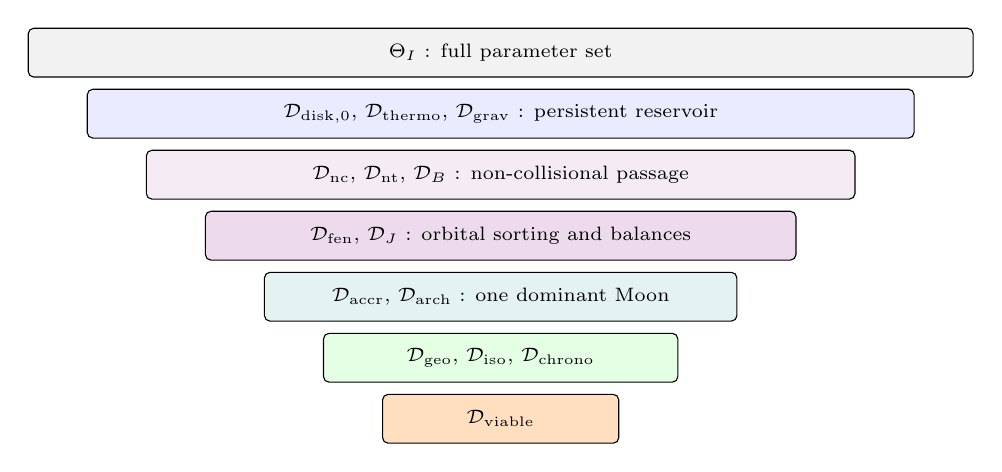
\begin{tikzpicture}[y=0.62cm]
  \foreach \w/\y/\lab/\c in {
     12/0/{$\Theta_I$ : full parameter set}/gray!10,
     10.5/-1.25/{$\mathcal{D}_{\mathrm{disk},0}$, $\mathcal{D}_{\mathrm{thermo}}$, $\mathcal{D}_{\mathrm{grav}}$ : persistent reservoir}/blue!8,
     9/-2.5/{$\mathcal{D}_{\mathrm{nc}}$, $\mathcal{D}_{\mathrm{nt}}$, $\mathcal{D}_B$ : non-collisional passage}/violet!8,
     7.5/-3.75/{$\mathcal{D}_{\mathrm{fen}}$, $\mathcal{D}_J$ : orbital sorting and balances}/violet!14,
     6/-5/{$\mathcal{D}_{\mathrm{accr}}$, $\mathcal{D}_{\mathrm{arch}}$ : one dominant Moon}/teal!10,
     4.5/-6.25/{$\mathcal{D}_{\mathrm{geo}}$, $\mathcal{D}_{\mathrm{iso}}$, $\mathcal{D}_{\mathrm{chrono}}$}/green!10,
     3/-7.5/{$\mathcal{D}_{\mathrm{viable}}$}/orange!25}
  { \node[draw,rounded corners=2pt,fill=\c,minimum width=\w cm,minimum height=0.62cm,font=\scriptsize]
      at (0,\y) {\lab}; }
\end{tikzpicture}
\caption{The viable domain as the intersection of successive gates. Only configurations that pass
all gates define the physical path.}
\label{fig:portes}
\end{figure}

% ---------------------------------------------------------------------
\chapter{Level I numerical program}
\label{ch:programme}
% ---------------------------------------------------------------------

The separation of time scales (Chapter~\ref{ch:chronologie}) allows the calculation to be divided
into three linked phases, throughout which each matter element preserves its dynamical, thermal and
chemical labels.

\section{Phase A: disk formation and evolution before \texorpdfstring{$B$}{B}}

The first simulation computes
\begin{equation}
\mathcal{A}(t)=\left\{\dot M_{\mathrm{in}},\ \Sigma(r,t),\ T(r,t),\ P(r,t),\ L_D(t),\
R_{\mathrm{out}}(t),\ \mathbf{X}(r,t),\ \mathbf{f}_{\mathrm{phase}}(r,t),\ Q_T(r,t),\ \mathcal{G}(t)\right\}.
\label{eq:phaseA}
\end{equation}
Its output is a family of states $\mathcal{D}_0$ accessible at time $t_B$.

\section{Phase B: grazing passage of \texorpdfstring{$B$}{B}}

The encounter, integrated with the exact field~\eqref{eq:adiff} and closed in the barycentric frame,
provides
\begin{equation}
\mathcal{B}=\left\{M_{D,1},\ L_{D,1},\ \Delta\mathbf{S}_\oplus,\ \Delta\mathbf{L}_{\mathrm{orb}},\
\Delta\mathbf{S}_B,\ M_{\oplus\to D},\ M_{B\to D},\ M_{\mathrm{esc}},\ i_{D,1},\ e_D(r),\ \chi_J,\ \mathcal{H}_{B,1}\right\}.
\label{eq:phaseB}
\end{equation}
The distribution of particles or fluid elements is summarized by
\begin{equation}
\Pi_{\mathrm{dyn}}=\Pi_{\mathrm{dyn}}\left(\varepsilon_{\mathrm{orb}},j_z,q_p,i,r_0,\lambda_\Omega,z
\,\middle|\,\Theta_I\right).
\label{eq:Pidyn}
\end{equation}

\section{Phase C: relaxation and accretion}

The final phase computes
\begin{equation}
\mathcal{C}=\left\{M_L,\ L_L,\ i_{L,0},\ \mathbf{X}_L,\ t_{\mathrm{acc},L},\ N_{\mathrm{sat}},\
f_{\mathrm{dom}},\ M_{\mathrm{reaccr}},\ M_{\mathrm{esc}}\right\}.
\label{eq:phaseC}
\end{equation}

\begin{figure}[htbp]
\centering
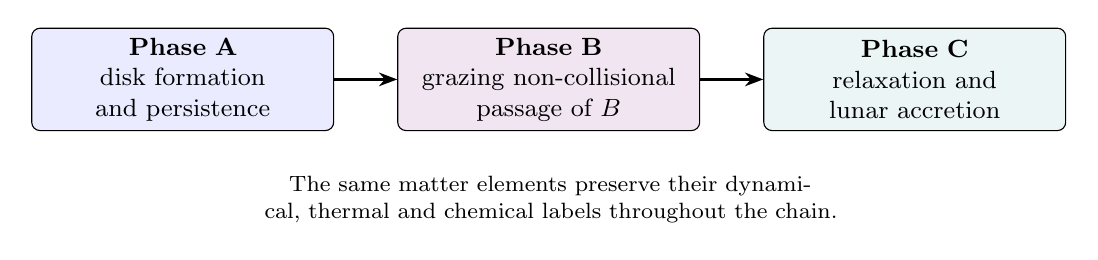
\begin{tikzpicture}[node distance=0.8cm,
  ph/.style={draw,rounded corners=3pt,align=center,font=\small,minimum height=1.3cm,text width=3.6cm,fill=#1}]
  \node[ph=blue!8] (A) {\textbf{Phase A}\\disk formation\\and persistence};
  \node[ph=violet!10,right=of A] (B) {\textbf{Phase B}\\grazing non-collisional\\passage of $B$};
  \node[ph=teal!8,right=of B] (C) {\textbf{Phase C}\\relaxation and\\lunar accretion};
  \draw[-{Stealth},thick] (A) -- (B);
  \draw[-{Stealth},thick] (B) -- (C);
  \node[font=\footnotesize,align=center,below=0.45cm of B,text width=13cm]
    {The same matter elements preserve their dynamical, thermal and chemical labels throughout the chain.};
\end{tikzpicture}
\caption{Architecture of the numerical program of the theory.}
\label{fig:programme}
\end{figure}

% =====================================================================

\section{Phase B protocol and viability maps}

\paragraph{Model.}
Reservoir elements are first treated as test particles in the field of the proto-Earth, while $B$
follows its exact hyperbola. The integration uses the differential acceleration~\eqref{eq:adiff}
and stops when criterion~\eqref{eq:atol} is satisfied. Each element is then classified according to
$(\varepsilon,\,j_z,\,e,\,q_p,\,r_{\mathrm{circ}})$ and criterion~\eqref{eq:fenetre}.

\paragraph{Response kernel.}
To decouple the response from the density profile, rings of elements are launched at about thirty
initial radii $r_0$ between $2$ and $5\,\Rt$, with several hundred azimuths each. This gives the
probability $P_k(r_0)$ that an element starting from $r_0$ ends in category
$k\in\{L,\mathrm{in},\mathrm{reaccr},\mathrm{esc},\to B\}$. For any profile $\Sigma(r_0)$,
\begin{equation}
\eta_k=\frac{1}{M_{D,0}}\int_{R_{\mathrm{in}}}^{R_{\mathrm{out}}}\Sigma(r_0)\,P_k(r_0)\,2\pi r_0\,\dd r_0.
\label{eq:noyau}
\end{equation}
A single integration per set of $B$ parameters can therefore be used for all reservoir profiles.

\paragraph{Reduced variables.}
The response depends on $\mu_B$, $q_B/\Rt$, $v_\infty/v_{\mathrm{esc}}$, $i_B$ and $\omega_B$. The
angular momentum ceded by the reservoir is obtained by weighting the elements; closure
\eqref{eq:fermeture} assigns the opposite to the orbit of $B$, which remains valid as long as
$M_D\ll M_B$.

\paragraph{Maps to produce.}
The viability maps are the main outputs of the program. They include the fractions
$\Delta\eta_L(q_B,i_B)$, $\eta_{\mathrm{esc}}(q_B,i_B)$ and $\eta_{\mathrm{reaccr}}(q_B,i_B)$ for
several values of $\mu_B$ and $v_\infty$; the exchanged fraction $\chi_J$; the latitude-depth
distribution of injected matter, $\dd M_{\oplus\to D}/\dd\lambda_\Omega\,\dd z$; and the
inclination $i_{D,1}$ of the reorganized reservoir. These maps are the results to be computed;
Figure~\ref{fig:tri} gives the analytical anticipation.
The same phase must preserve the post-passage heliocentric orbit $\mathcal{H}_{B,1}$ so that a
later calculation can test the gate $\mathcal{D}_{B,\mathrm{hel}}$.

\section{First pilot calculation of orbital sorting}
\label{sec:pilot-etaL}

A first Phase~B calculation was performed to verify that the lunar window
\eqref{eq:fenetre} can be reached over a non-punctual domain of parameters. It is not a
hydrodynamical proof: the reservoir is represented by $1152$ equal-mass test particles,
initially circular and coplanar, distributed between $1.6$ and $2.9\,\Rt$ with
$\Sigma\propto r^{-1}$. The Roche limit is set to $a_{\mathrm{Roche}}=2.903\,\Rt$, the
equatorial radius to $\Req=1.20\,\Rt$, the mass of $B$ to $M_B=0.10\,\Mt$, and the
asymptotic velocity to $v_\infty=2$~km\,s$^{-1}$. The passage is prograde, with
$\omega_B=90^\circ$, and the acceleration used is the exact differential field of
Eq.~\eqref{eq:adiff}.

\begin{table}[htbp]
\centering
\small
\caption{Pilot map of the fraction $100\eta_L$ placed in the lunar window. Test-particle
calculation, without disk self-gravity, without mutual collisions, without pressure and without
hydrodynamics.}
\label{tab:pilot-etaL}
\begin{tabular}{c|ccccc}
\toprule
$i_B$ & $q_B=2.8\,\Rt$ & $3.0\,\Rt$ & $3.2\,\Rt$ & $3.4\,\Rt$ & $3.6\,\Rt$ \\
\midrule
$18^\circ$ & 13.5 & 11.4 & 9.7 & 9.0 & 7.3 \\
$21^\circ$ & 14.2 & 12.7 & 10.3 & 8.9 & 8.0 \\
$24^\circ$ & 15.7 & 12.7 & 11.2 & 9.4 & 7.8 \\
$27^\circ$ & 16.1 & 13.5 & 10.8 & 9.7 & 8.1 \\
$30^\circ$ & 17.1 & 14.5 & 11.3 & 10.3 & 8.7 \\
\bottomrule
\end{tabular}
\end{table}

\begin{figure}[htbp]
\centering
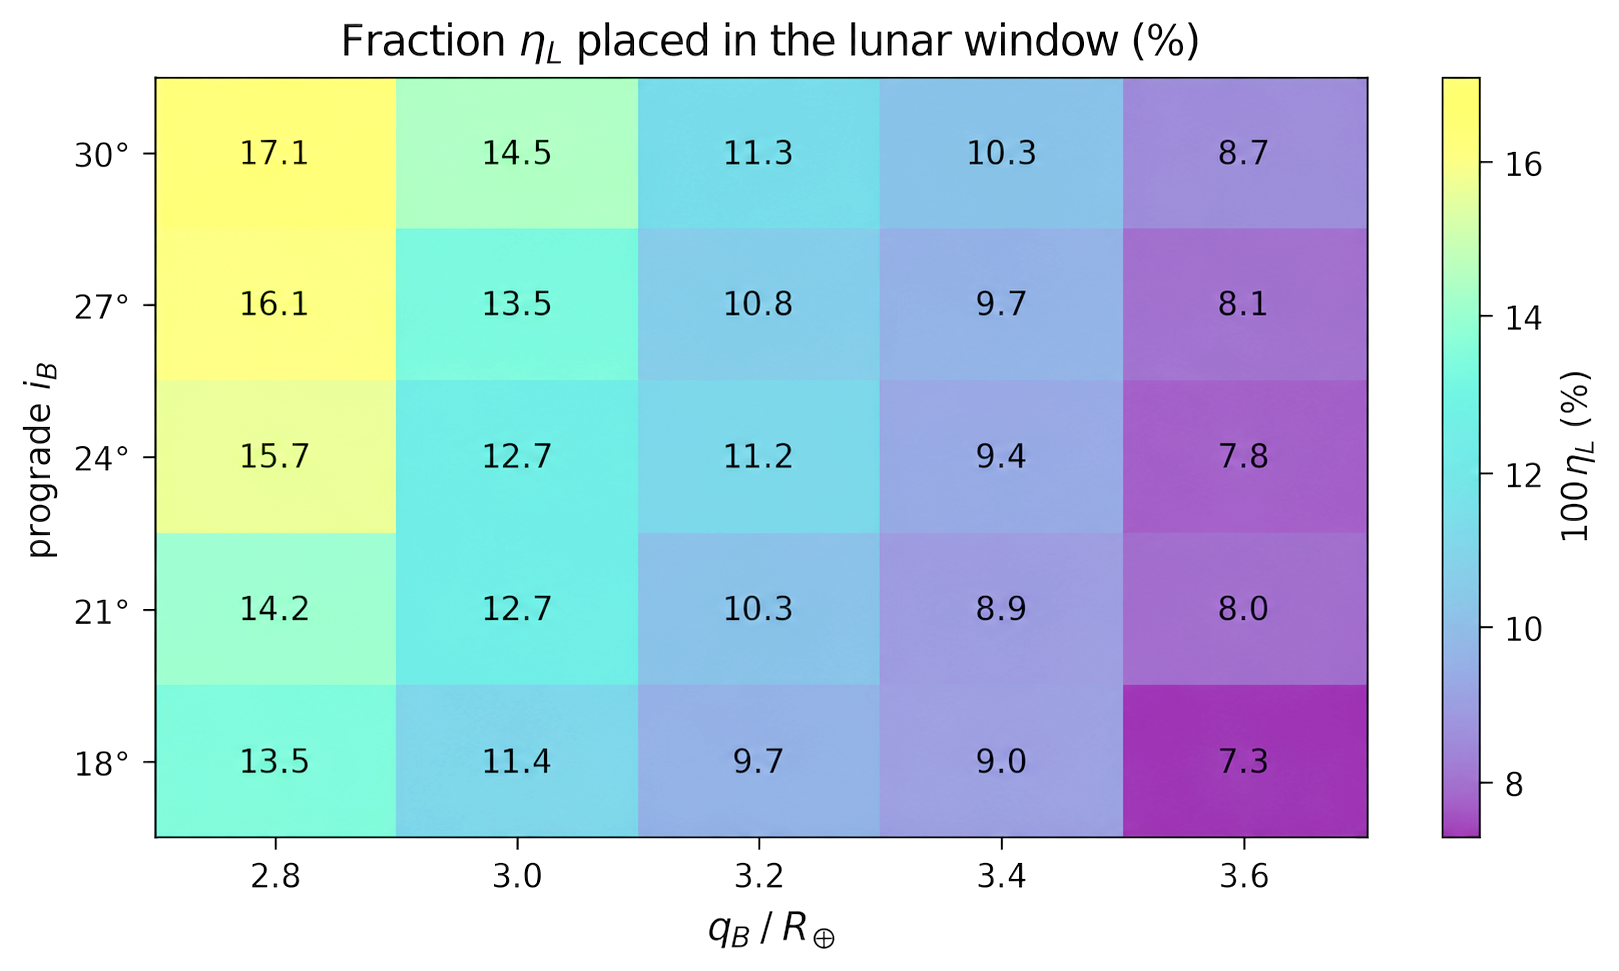
\includegraphics[width=0.82\textwidth]{Map_etal_driver.png}
\caption{Pilot map of $\eta_L(q_B,i_B)$ for $M_B=0.10\,\Mt$,
$v_\infty=2$~km\,s$^{-1}$ and $\omega_B=90^\circ$. The map illustrates the existence of a
continuous response band, to be confirmed by massive, collisional and self-gravitating simulations.}
\label{fig:pilot-etaL}
\end{figure}

For the case $q_B=3\,\Rt$ and $i_B=30^\circ$, the calculation gives
\begin{equation}
\eta_L=0.145,\qquad \eta_{\mathrm{esc}}=0.023,\qquad
\eta_{\mathrm{reaccr}}=0.019,\qquad \eta_{\to B}=0.023.
\label{eq:pilot-case}
\end{equation}
The remaining fraction, $0.789$, remains bound in the inner domain or in states that do not
immediately satisfy the lunar window. For a fixed initial mass, the mass directly placed in the
window is
\begin{equation}
M_{L,\mathrm{window}}\simeq0.145\,M_{D,0},
\label{eq:MLwindow}
\end{equation}
which means that one lunar mass immediately placed in this window would require
$M_{D,0}\simeq6.9\,M_L$ in this test calculation. For $q_B=2.8\,\Rt$ and $i_B=30^\circ$, the value
$\eta_L=0.171$ lowers this mass to $M_{D,0}\simeq5.85\,M_L$.

The retrograde control isolates the role of passage direction. For $q_B=3\,\Rt$, at identical
periastron latitude and with the other parameters unchanged, one obtains
\begin{equation}
\eta_{L,\mathrm{retro}}\simeq0.027,
\label{eq:retro-pilot}
\end{equation}
that is, an efficiency about $5.4$ times lower than in the prograde case. This result is consistent
with the coherence-duration argument of Eq.~\eqref{eq:prograde}.

The radial origin of the matter promoted into the lunar window confirms that sorting acts mainly
on the external part of the reservoir, close to Roche: for the case $q_B=3\,\Rt$, $i_B=30^\circ$,
the contributions to the $\eta_L$ cohort come $35.0\%$ from the $2.53$--$2.71\,\Rt$ annulus and
$53.1\%$ from the $2.71$--$2.90\,\Rt$ annulus.

\begin{controle}
The pilot calculation provides a concrete positive signal: the lunar window is not empty in the
tested region, and the prograde low-latitude configuration is much more efficient than the
retrograde control. It does not yet prove viability, because self-gravity, collisions,
hydrodynamics, thermal evolution and balance closure still have to be added. Its role is to identify
the promising region of parameter space to be explored by Level~I.
\end{controle}

\begin{falsif}
If, on the full grid, $\Delta\eta_L$ remains negligible, or only increases at the cost of an escaped
fraction incompatible with the reservoir mass, the orbital-sorting mechanism is insufficient and
the corresponding branch is excluded.
\end{falsif}

\begin{rappel}
The viability domain fixes what the calculation must demonstrate. The final part states what
nature should show if the theory is correct, and how to verify it.
\end{rappel}

% =====================================================================
\part{Predictions}
\label{part:predictions}
% =====================================================================

\noindent
Each prediction is stated in the same form: what should be observed \emph{if the theory is correct},
and then \emph{how to verify it}, through measurement of lunar samples or through calculation. The
predictions concern architecture, composition, chronology and dynamics.

% ---------------------------------------------------------------------
\chapter{Predictions and verification}
\label{ch:predictions}
\label{sec:signatures}
% ---------------------------------------------------------------------

\begin{prediction}{P1. One dominant satellite}
\sila The sorted and relaxed reservoir produces a satellite mass almost entirely concentrated in one
body:
\begin{equation}
\mathcal{D}_{\mathrm{arch}}=\left\{\Theta_I:\ M_L\simeq M_{L,\mathrm{obs}},\
N_{\mathrm{sat,large}}\simeq1,\ f_{\mathrm{dom}}\to1\right\}.
\label{eq:Darch}
\end{equation}
\verif Phase~C $N$-body simulations, with collisions and self-gravity, starting from the reservoirs
reorganized in Phase~B; tracking of $N_{\mathrm{sat}}$ and $f_{\mathrm{dom}}$.
\end{prediction}

\begin{prediction}{P2. A negligible share of \texorpdfstring{$B$}{B}}
\sila The fraction of lunar matter derived from $B$,
\begin{equation}
f_B=\frac{M_{B\to L}}{M_L},
\label{eq:fB}
\end{equation}
is small, and the oxygen, titanium and chromium isotopic compositions of the Moon are
indistinguishable from those of the silicate Earth within the limits~\eqref{eq:bornefB}.
\verif High-precision isotopic measurements on varied lunar samples; calculation of $M_{B\to D}$ in
Phase~B for passages with $q_B$ close to $d_{R,B}$.
\end{prediction}

\begin{prediction}{P3. Terrestrial tungsten}
\sila After correction for late accretion, lunar $\varepsilon^{182}$W is identical to that of Earth's
mantle, and the Hf/W ratio of lunar matter does not produce a $^{182}$W excess incompatible with
time $t_B$.
\verif Measurements of $\varepsilon^{182}$W and Hf/W on lunar rocks with low cosmic-ray exposure;
comparison with the Phase~A chronology.
\end{prediction}

\begin{prediction}{P4. Inheritance from terrestrial core segregation}
\sila Lunar depletions in V, Cr and Mn reproduce those of Earth's mantle, and the lunar W/U ratio is
close to the terrestrial ratio.
\verif Estimates of lunar-mantle composition from basalts and primitive rocks; high-pressure
metal--silicate partitioning experiments.
\end{prediction}

\begin{prediction}{P5. A dynamical--chemical correlation}
\sila The same matter cohort carries both an orbital history and a composition:
\begin{equation}
(r_0,\lambda_\Omega,z)\longleftrightarrow(\varepsilon_{\mathrm{orb}},j_z,q_p,\mathbf{X}),
\label{eq:correlation}
\end{equation}
and the W/V ratio of injected matter~\eqref{eq:WV} reflects the depth and latitude from which it was
stripped.
\verif Tracking of the labels $(\lambda_\Omega,z)$ in Phase~B; comparison of computed W/V with
measured ratios normalized to elements of similar behavior.
\end{prediction}

\begin{prediction}{P6. A reservoir of terrestrial composition}
\sila The preexisting circumterrestrial reservoir is terrestrial silicate in nature, fed mainly by
equatorial mass loss and mantle ejecta, and the lunar FeO excess is produced by internal
transformations within the reservoir.
\verif Phase~A balances on the channels~\eqref{eq:canaux}; calculation of $\boldsymbol{\Pi}_D$ and
comparison with lunar FeO and siderophile contents.
\end{prediction}

\begin{prediction}{P7. A non-zero initial inclination}
\sila A slightly inclined passage gives the reorganized reservoir an angular momentum not collinear
with Earth's spin:
\begin{equation}
i_{D,1}=\arccos\!\left(\frac{\mathbf{L}_{D,1}\cdot\mathbf{S}_{\oplus,1}}
{|\mathbf{L}_{D,1}|\,|\mathbf{S}_{\oplus,1}|}\right).
\label{eq:inclinaison}
\end{equation}
This quantity constitutes an initial condition for the tidal evolution of the Earth--Moon system,
whose lunar orbital inclination is one of the classical enigmas \cite{PahlevanMorbidelli2015}.
\verif Calculation of $i_{D,1}$ in Phase~B, then integration of tidal evolution up to the present
orbit.
\end{prediction}

\begin{prediction}{P8. Compatible angular momentum}
\sila The angular momentum of the Earth--reservoir system left by the passage, $J_{\oplus D,1}$, is
compatible with that of the Earth--Moon system, accounting for its later evolution.
\verif Closure of balance~\eqref{eq:fermeture} in Phase~B; comparison of $J_{\oplus D,1}$ with
$L_{\mathrm{EM}}$.
\end{prediction}

\begin{prediction}{P9. Efficient orbital sorting in the dynamical low-latitude band}
\sila There exists a continuous region of the prograde low-latitude band in which $\Delta\eta_L$ is
significant and $\eta_{\mathrm{esc}}$ moderate, in accordance with~\eqref{eq:fenetre-succes}.
\verif Phase~B viability maps (Chapter~\ref{ch:programme}).
\end{prediction}

% =====================================================================
\begin{prediction}{P10. An eliminated heliocentric fate for \texorpdfstring{$B$}{B}}
\sila Planet $B$ belongs to the population of primordial planetary bodies later eliminated:
\begin{equation}
B\in\mathcal{P}_{\mathrm{elim}},\qquad t_B<t_{\mathrm{ej}},
\label{eq:predB}
\end{equation}
and the post-passage heliocentric orbit $\mathcal{H}_{B,1}$ is compatible with later diffusion toward
collision, accretion by a planet or ejection from the Solar System.
\verif Heliocentric $N$-body integrations starting from $\mathcal{H}_{B,1}$, with both early and late
instability scenarios, and verification that the final architectures remain compatible with the
present Solar System.
\end{prediction}

\chapter*{General conclusion}
\addcontentsline{toc}{part}{General conclusion}
\markboth{General conclusion}{General conclusion}
% =====================================================================

The question asked at the beginning of this work was that of a path: how could the Earth--Moon
system observed today have emerged from the proto-terrestrial system through a physically coherent
evolution?

The theory proposes a precise answer. During its growth, the proto-Earth is accompanied by a
secondary circumterrestrial reservoir, analogous in principle to the accretion systems of giant
planets and to the disk of PDS~70c, but dominated by solids and fed mainly by its own silicate
layer. This reservoir already contains mass and angular momentum when planet $B$ passes.

$B$ is neither an impactor nor the main supplier of lunar matter. It is a transient gravitational
agent redistributing mass and angular-momentum fluxes between the reservoirs. Grazing passages are
at least as frequent as collisions (Eq.~\eqref{eq:frequence}); the trajectory of $B$ carries an
angular momentum of the same order as that of the Earth--Moon system (Eq.~\eqref{eq:LBrel}); in the
low-latitude band of an oblate, rapidly rotating proto-Earth, its prograde passage injects
superficial matter already depleted in metal. Its central result is orbital sorting: a bound cohort
is placed by the torque of $B$ in the lunar window beyond the Roche limit (Eqs.~\eqref{eq:fenetre}
and~\eqref{eq:etaL}), while other fractions re-accrete or escape.

The sorted reservoir relaxes and accretes the Moon, concentrating satellite mass into a dominant
body. Geochemistry belongs to the same story: the non-collisional passage favors a small
contribution from $B$, making isotopic similarity an expected constraint of the viable domain;
vanadium and tungsten, read together, trace the fluxes of terrestrial silicate matter and the depth
of the sampled layer.


The logic of the model closes with the fate of $B$. The agent that reorganizes the circumterrestrial
reservoir need not remain in the final Solar System: it may belong to the population of primordial
planetary bodies later eliminated by the global orbital instability, provided that its passage
satisfies $t_B<t_{\mathrm{ej}}$. This hypothesis links Earth--Moon formation to migration and
instability in the primordial Solar System without requiring $B$ to be identified with a single
specific missing planet.

The final scientific question is
\begin{equation}
\boxed{\;\mathcal{S}_0=\{\Theta_I\}\longrightarrow\mathcal{D}_0
\xrightarrow{\;\text{orbital sorting by }B\;}\mathcal{D}_1\longrightarrow
\left(M_L,\,L_L,\,i_{L,0},\,\mathbf{X}_L\right)\in\mathcal{D}_{\mathrm{viable}}
\longrightarrow\mathcal{S}_f.\;}
\label{eq:question}
\end{equation}
The theory does not claim to demonstrate a unique history. It defines a quantitative and
falsifiable physical path, and indicates, for each of its stages, how to confirm, restrict or
exclude it.

% =====================================================================
\appendix
% =====================================================================

\chapter{Demonstrations}
\label{app:demo}

\section{Circularization radius of captured matter}
\label{app:rc}

Matter captured through an accretion zone of radius $R_{\mathrm{acc}}$ in a sheared flow of
frequency $\Omega$ carries a specific angular momentum of order $j\simeq\Omega R_{\mathrm{acc}}^2/4$
\cite{QuillenTrilling1998}. It circularizes at the radius where its angular momentum equals the
Keplerian value, $j^2=G\Mt r_c$:
\begin{equation}
r_c=\frac{\Omega^2R_{\mathrm{acc}}^4}{16\,G\Mt}.
\end{equation}
For $R_{\mathrm{acc}}=R_H$, the definition of the Hill radius, $R_H^3=G\Mt/(3\Omega^2)$, gives
$\Omega^2=G\Mt/(3R_H^3)$ and $r_c=R_H/48$. For accretion limited to the Bondi sphere, $r_c$ is
multiplied by $(R_{\mathrm{B}}/R_H)^4$, leading to Eq.~\eqref{eq:rc}.

\section{Frequency of grazing passages}

For a hyperbolic trajectory with impact parameter $b$, conservation of angular momentum and energy
gives $b\,v_\infty=q\,v_p$ and $v_p^2=v_\infty^2+2G\Mtot/q$, hence
\begin{equation}
b^2=q^2\left(1+\frac{2G\Mtot}{q\,v_\infty^2}\right),\qquad \sigma(q)=\pi b^2,
\end{equation}
which is Eq.~\eqref{eq:sigma}. With $\Theta=2G\Mtot/(R_cv_\infty^2)$,
$\sigma(R_c)=\pi R_c^2(1+\Theta)$ and $\sigma(2R_c)=\pi R_c^2(4+2\Theta)$; the ratio
$[\sigma(2R_c)-\sigma(R_c)]/\sigma(R_c)=(3+\Theta)/(1+\Theta)$ decreases from 3 to 1 as $\Theta$
increases from 0 to infinity.

\section{Trajectory nodes and non-crossing}

The equation of the conic is $r=p/(1+e\cos\nu)$ with $p=q(1+e)$. The trajectory crosses the
reference plane when the argument of latitude $\omega+\nu$ is $0$ or $\pi$, i.e. $\nu=-\omega$ or
$\nu=\pi-\omega$; the corresponding radii are $p/(1+e\cos\omega)$ and $p/(1-e\cos\omega)$, whose
smaller value is $p/(1+e|\cos\omega|)$. This is Eq.~\eqref{eq:nontraversee}.

\section{Circularization radius and perigee}
\label{app:rcirc}

For a bound orbit, $j^2=G\Mt\,a(1-e^2)$ and $q_p=a(1-e)$, hence
$r_{\mathrm{circ}}=j^2/(G\Mt)=a(1-e)(1+e)=q_p(1+e)$. Since $0\le e<1$,
$q_p\le r_{\mathrm{circ}}<2q_p$, which establishes Eq.~\eqref{eq:rcirc-qp}.

\section{Orbital-sorting boundaries}
\label{app:tri}

An element on a circular orbit of radius $r_0$ has velocity $v_K=\sqrt{G\Mt/r_0}$. After a tangential
impulse, $v=v_K(1+\delta)$ and $j=r_0v_K(1+\delta)$, hence
$r_{\mathrm{circ}}=r_0(1+\delta)^2$. Its specific energy is
\begin{equation}
\varepsilon=\frac{G\Mt}{r_0}\left[\frac{(1+\delta)^2}{2}-1\right],
\end{equation}
which vanishes for $(1+\delta)^2=2$: $\delta_{\mathrm{esc}}=\sqrt2-1$. For $\delta<0$, $r_0$ becomes
the apogee; the semi-major axis is $a=r_0/[2-(1+\delta)^2]$ and the perigee is
$q_p=2a-r_0=r_0(1+\delta)^2/[2-(1+\delta)^2]$. The condition $q_p=\Req$ gives
$(1+\delta)^2=2\Req/(r_0+\Req)$, hence $\delta_{\mathrm{re}}$. The condition
$r_{\mathrm{circ}}=\aR$ gives $\delta_L=\sqrt{\aR/r_0}-1$. This gives Eq.~\eqref{eq:frontieres}.

\section{Tidal impulse}
\label{app:impulsion}

In the approximation of a rapid rectilinear trajectory with velocity $V$ and parameter $b$, the
proto-Earth and an element located at relative position $\mathbf{r}$ receive impulses whose
difference, to first order in $r/b$, has an amplitude at most of order $2GM_Br/(b^2V)$
\cite{Spitzer1958,BinneyTremaine2008}. With $b=q_B$, $V=v_p=\sqrt{2G\Mtot/q_B}$ and
$v_K=\sqrt{G\Mt/r}$:
\begin{equation}
\frac{\Delta v}{v_K}\sim\frac{2\mu_B\sqrt{G\Mt}\,r^{3/2}}{q_B^2v_p}
=\sqrt2\,\frac{\mu_B}{\sqrt{1+\mu_B}}\left(\frac{r}{q_B}\right)^{3/2}.
\end{equation}
This estimate assumes $r<q_B$ and impulsive forcing; it neglects trajectory curvature and
therefore gives an order of magnitude, replaced in Phase~B by the exact calculation.

\section{Circularization energy}

A parcel with energy $\varepsilon_i=-G\Mt/(2a)$ circularizes at conserved angular momentum at radius
$a_{\mathrm{circ}}=a(1-e^2)$, with energy $\varepsilon_f=-G\Mt/(2a_{\mathrm{circ}})$. The released
energy is
$\varepsilon_i-\varepsilon_f=\frac{G\Mt}{2a}\left[\frac{1}{1-e^2}-1\right]=\frac{G\Mt}{2a}\frac{e^2}{1-e^2}$,
which is Eq.~\eqref{eq:circ}.

\section{Injection threshold}

At the sub-$B$ point, the radial tidal acceleration is, for $\lambda_B=0$,
\begin{equation}
GM_B\left[(q_B-\Req)^{-2}-q_B^{-2}\right]\simeq2GM_B\Req/q_B^3.
\end{equation}
At low latitude, its projection on the radial direction is multiplied by
$F(\lambda_B)=(3\cos^2\lambda_B-1)/2$. Equating it to the effective gravity
$(G\Mt/\Req^2)(1-\tilde\omega^2)$ gives
\begin{equation}
1-\tilde\omega^2\lesssim2F(\lambda_B)\,\frac{M_B}{\Mt}\left(\frac{\Req}{q_B}\right)^3,
\end{equation}
which is Eq.~\eqref{eq:seuil}.

\section{Bound on the chondritic share of the reservoir}
\label{app:borneW}

With $f_B=0$ and $\varepsilon^{182}\mathrm{W}_\oplus=0$, Eq.~\eqref{eq:melange} becomes
$\varepsilon^{182}\mathrm{W}_L=f_0C_{\mathrm{W},0}\varepsilon^{182}\mathrm{W}_0/
[f_0C_{\mathrm{W},0}+(1-f_0)C_{\mathrm{W},\oplus}]$. For
$f_0C_{\mathrm{W},0}\ll C_{\mathrm{W},\oplus}$, the denominator reduces to $C_{\mathrm{W},\oplus}$,
and the condition $|\varepsilon^{182}\mathrm{W}_L|<\delta\varepsilon$ gives
Eq.~\eqref{eq:bornef0}.

% ---------------------------------------------------------------------
\chapter{Notation}
\label{app:notations}
% ---------------------------------------------------------------------

\small
\begin{longtable}{>{\raggedright\arraybackslash}p{3.2cm}>{\raggedright\arraybackslash}p{11.6cm}}
\toprule
\textbf{Symbol} & \textbf{Meaning} \\
\midrule
\endhead
$\mathcal{S}_0$, $\mathcal{S}_f$ & initial state of the proto-terrestrial system, observed state \\
$\RT$, $\RD$, $\RB$, $\Rinf$ & reservoirs: proto-Earth, circumterrestrial reservoir, planet $B$, external medium \\
$\Phi_{i\to j}$ & mass flux from reservoir $i$ to reservoir $j$ \\
$\boldsymbol{\mathcal{T}}_{j\to i}$ & torque exerted by reservoir $j$ on reservoir $i$ \\
$\mathbf{X}_i$, $\mathbf{X}_{i\to j}$ & composition of a reservoir, composition of a flux \\
$\Mt$, $\Req$, $\Omega_\oplus$, $S_\oplus$ & mass, equatorial radius, angular velocity and spin of the proto-Earth \\
$\tilde\omega$ & reduced rotation $\Omega_\oplus/\sqrt{G\Mt/\Req^3}$ \\
$J_2$ & gravitational flattening coefficient \\
$M_D$, $L_D$, $\Sigma(r)$ & mass, angular momentum and surface density of the reservoir \\
$\mathcal{D}_0$, $\mathcal{D}_1$ & reservoir state before and after the encounter \\
$\mathcal{G}(t)$ & population of aggregates and moonlets \\
$R_{\mathrm{in}}$, $R_{\mathrm{out}}$ & inner and outer radii of the reservoir \\
$R_H$, $R_{\mathrm{B}}$ & Hill and Bondi radii \\
$\aR$, $a_{\mathrm{sync}}$ & Roche limit, synchronous orbit \\
$M_B$, $\mu_B$, $R_B$, $\rho_B$ & mass, relative mass, radius and density of $B$ \\
$q_B$, $v_\infty$, $v_p$, $e_B$ & periastron, asymptotic velocity, periastron velocity, eccentricity of $B$'s trajectory \\
$i_B$, $\omega_B$ & inclination relative to the rotational equator, argument of periastron \\
$\lambda_B$ & latitude of the sub-$B$ point at periastron \\
$\lambda_c$ & half-width of the dynamical low-latitude band \\
$t_{\mathrm{enc}}$, $\eta(r)$ & encounter duration, regime parameter $\Omega_Kt_{\mathrm{enc}}$ \\
$d_{R,B}$ & Roche distance of $B$ around the proto-Earth \\
$L_{B,\mathrm{rel}}$, $\chi_J$ & relative orbital angular momentum of $B$, exchanged fraction \\
$\varepsilon$, $j$, $j_z$, $e$, $q_p$ & energy, angular momentum, projection, eccentricity and perigee of an element \\
$r_{\mathrm{circ}}$ & circularization radius $j^2/(G\Mt)$ \\
$\eta_L$, $\Delta\eta_L$ & fraction in the lunar window, specific contribution of $B$ \\
$\eta_{\mathrm{in}}$, $\eta_{\mathrm{reaccr}}$, $\eta_{\mathrm{esc}}$, $\eta_{\to B}$ & fractions: inner disk, re-accretion, escape, capture by $B$ \\
$\delta$ & relative tangential impulse $\Delta v_t/v_K$ \\
$f_0$, $f_\oplus$, $f_B$ & provenance fractions of lunar matter \\
$f_{\mathrm{dom}}$, $N_{\mathrm{sat}}$ & dominance factor, number of satellites \\
$\lambda_\Omega$, $z$ & dynamical latitude and depth of origin of injected matter \\
$\mathcal{P}_{\mathrm{elim}}$ & population of primordial planetary bodies later eliminated by collision, accretion, diffusion or ejection \\
$t_{\mathrm{ej}}$ & time of ejection or dynamical elimination of $B$ \\
$\mathcal{H}_{B,1}$ & heliocentric orbit of $B$ after its passage near the proto-Earth \\
$\Theta_I$ & Level I parameter vector \\
$\mathcal{D}_{\mathrm{viable}}$ & viability domain \\
$\mathcal{D}_{B,\mathrm{hel}}$ & heliocentric gate checking the eliminated fate of $B$ \\
\bottomrule
\end{longtable}
\normalsize

% ---------------------------------------------------------------------
\chapter{Constants and numerical values}
\label{app:constantes}
% ---------------------------------------------------------------------

\begin{table}[htbp]
\centering
\small
\caption{Constants and reference values used in the work.}
\label{tab:constantes}
\begin{tabular}{lll}
\toprule
\textbf{Quantity} & \textbf{Symbol} & \textbf{Value} \\
\midrule
Terrestrial gravitational parameter & $G\Mt$ & $3.986\times10^{14}$ m$^3$\,s$^{-2}$ \\
Earth mass & $\Mt$ & $5.972\times10^{24}$ kg \\
Mean Earth radius & $\Rt$ & $6.371\times10^{6}$ m \\
Moon mass & $M_L$ & $7.342\times10^{22}$ kg \\
Solar mass & $M_\odot$ & $1.989\times10^{30}$ kg \\
Astronomical unit & $a_\oplus$ & $1.496\times10^{11}$ m \\
Mean lunar density & $\rho_s$ & $3.34$ g\,cm$^{-3}$ \\
Mean terrestrial density & $\bar\rho_\oplus$ & $5.51$ g\,cm$^{-3}$ \\
Earth--Moon angular momentum & $L_{\mathrm{EM}}$ & $\approx3.5\times10^{34}$ kg\,m$^2$\,s$^{-1}$ \\
Roche limit ($\rho_s=3.34$) & $\aR$ & $\approx2.9\,\Rt$ \\
Half-life of $^{182}$Hf & $t_{1/2}$ & $8.9$ Ma \\
\bottomrule
\end{tabular}
\end{table}

\clearpage
\phantomsection
\addcontentsline{toc}{part}{Bibliography}
\markboth{Bibliography}{Bibliography}
\begin{thebibliography}{99}
\small

\bibitem{Pringle1981} J.~E. Pringle, ``Accretion discs in astrophysics'', \emph{Annual Review of
Astronomy and Astrophysics}, 19 (1981), 137--160. doi:10.1146/annurev.aa.19.090181.001033.

\bibitem{JohansenLacerda2010} A. Johansen and P. Lacerda, ``Prograde rotation of protoplanets by
accretion of pebbles in a gaseous environment'', \emph{Monthly Notices of the Royal Astronomical
Society}, 404 (2010), 475--485. doi:10.1111/j.1365-2966.2010.16309.x.

\bibitem{Visser2020} R.~G. Visser, C.~W. Ormel, C. Dominik and S. Ida, ``Spinning up planetary
bodies by pebble accretion'', \emph{Icarus}, 335 (2020), 113380. doi:10.1016/j.icarus.2019.07.014.

\bibitem{Johansen2021} A. Johansen, T. Ronnet, M. Bizzarro, M. Schiller, M. Lambrechts,
Å. Nordlund and H. Lammer, ``A pebble accretion model for the formation of the terrestrial planets
in the Solar System'', \emph{Science Advances}, 7 (2021), eabc0444. doi:10.1126/sciadv.abc0444.

\bibitem{CanupWard2006} R.~M. Canup and W.~R. Ward, ``A common mass scaling for satellite systems
of gaseous planets'', \emph{Nature}, 441 (2006), 834--839. doi:10.1038/nature04860.

\bibitem{Toomre1964} A. Toomre, ``On the gravitational stability of a disk of stars'',
\emph{The Astrophysical Journal}, 139 (1964), 1217--1238. doi:10.1086/147861.

\bibitem{Ida1997} S. Ida, R.~M. Canup and G.~R. Stewart, ``Lunar accretion from an impact-generated
disk'', \emph{Nature}, 389 (1997), 353--357. doi:10.1038/38669.

\bibitem{SalmonCanup2012} J. Salmon and R.~M. Canup, ``Lunar accretion from a Roche-interior fluid
disk'', \emph{The Astrophysical Journal}, 760 (2012), 83. doi:10.1088/0004-637X/760/1/83.

\bibitem{CanupWard2002} R.~M. Canup and W.~R. Ward, ``Formation of the Galilean satellites:
conditions of accretion'', \emph{The Astronomical Journal}, 124 (2002), 3404--3423.
doi:10.1086/344684.

\bibitem{Nimmo2026} F. Nimmo, R. Canup, Y. Fujii, A. Izidoro, J. Ji, W. McKinnon, O. Mousis,
C. Ormel, M. Ogihara, D. Stevenson and M. Blanc, ``Origin and evolution of the Galilean satellites
within the Jovian system'', \emph{Space Science Reviews}, 222 (2026), article~46.
doi:10.1007/s11214-026-01295-6.

\bibitem{Charnoz2010} S. Charnoz, J. Salmon and A. Crida, ``The recent formation of Saturn's
moonlets from viscous spreading of the main rings'', \emph{Nature}, 465 (2010), 752--754.
doi:10.1038/nature09096.

\bibitem{Blanc2025} M. Blanc, A. Crida, Y. Shibaike, S. Charnoz, M. El~Moutamid, P. Estrada,
O. Mousis, J. Salmon, A. Schneeberger and P. Vernazza, ``Understanding the formation of Saturn's
regular moons in the context of giant planet moons formation scenarios'', \emph{Space Science
Reviews}, 221 (2025), article~35. doi:10.1007/s11214-025-01156-8.

\bibitem{Helled2020} R. Helled, N. Nettelmann and T. Guillot, ``Uranus and Neptune: origin,
evolution and internal structure'', \emph{Space Science Reviews}, 216 (2020).
doi:10.1007/s11214-020-00660-3.

\bibitem{Benisty2021} M. Benisty, J. Bae, S. Facchini, M. Keppler, R. Teague, A. Isella,
N.~T. Kurtovic, L.~M. Pérez, A. Sierra, S.~M. Andrews et al., ``A circumplanetary disk around
PDS70c'', \emph{The Astrophysical Journal Letters}, 916 (2021), L2. doi:10.3847/2041-8213/ac0f83.

\bibitem{JPL} Jet Propulsion Laboratory, Solar System Dynamics, ``Planetary satellite physical
parameters and mean elements'', JPL/Caltech, data accessed September 2026.

\bibitem{Popovas2018} A. Popovas, Å. Nordlund, J.~P. Ramsey and C.~W. Ormel, ``Pebble dynamics and
accretion on to rocky planets -- I. Adiabatic and convective models'', \emph{Monthly Notices of the
Royal Astronomical Society}, 479 (2018), 5136--5156. doi:10.1093/mnras/sty1752.

\bibitem{Ruskol1960} E.~L. Ruskol, ``The origin of the Moon. I. Formation of a swarm of bodies
around the Earth'', \emph{Soviet Astronomy}, 4 (1960), 657.

\bibitem{Weidenschilling1986} S.~J. Weidenschilling, R. Greenberg, C.~R. Chapman, F. Herbert,
D.~R. Davis, M.~J. Drake, J. Jones and W.~K. Hartmann, ``Origin of the Moon from a circumterrestrial
disk'', in W.~K. Hartmann, R.~J. Phillips and G.~J. Taylor (eds.), \emph{Origin of the Moon}, Lunar
and Planetary Institute, Houston (1986), 519--550.

\bibitem{HartmannDavis1975} W.~K. Hartmann and D.~R. Davis, ``Satellite-sized planetesimals and
lunar origin'', \emph{Icarus}, 24 (1975), 504--515.

\bibitem{CameronWard1976} A.~G.~W. Cameron and W.~R. Ward, ``The origin of the Moon'',
\emph{Lunar Science VII} (1976), 120--122.

\bibitem{CanupAsphaug2001} R.~M. Canup and E. Asphaug, ``Origin of the Moon in a giant impact near
the end of the Earth's formation'', \emph{Nature}, 412 (2001), 708--712. doi:10.1038/35089010.

\bibitem{Canup2004} R.~M. Canup, ``Simulations of a late lunar-forming impact'', \emph{Icarus},
168 (2004), 433--456. doi:10.1016/j.icarus.2003.09.028.

\bibitem{CukStewart2012} M. Ćuk and S.~T. Stewart, ``Making the Moon from a fast-spinning Earth:
a giant impact followed by resonant despinning'', \emph{Science}, 338 (2012), 1047--1052.
doi:10.1126/science.1225542.

\bibitem{Canup2012} R.~M. Canup, ``Forming a Moon with an Earth-like composition via a giant
impact'', \emph{Science}, 338 (2012), 1052--1055. doi:10.1126/science.1226073.

\bibitem{Lock2018} S.~J. Lock, S.~T. Stewart, M.~I. Petaev, Z. Leinhardt, M.~T. Mace,
S.~B. Jacobsen and M. Ćuk, ``The origin of the Moon within a terrestrial synestia'', \emph{Journal
of Geophysical Research: Planets}, 123 (2018), 910--951. doi:10.1002/2017JE005333.

\bibitem{Mitler1975} H.~E. Mitler, ``Formation of an iron-poor moon by partial capture, or: yet
another exotic theory of lunar origin'', \emph{Icarus}, 24 (1975), 256--268.

\bibitem{QuillenTrilling1998} A.~C. Quillen and D.~E. Trilling, ``Do proto-Jovian planets drive
outflows?'', \emph{The Astrophysical Journal}, 508 (1998), 707--713.

\bibitem{MartinLubow2011} R.~G. Martin and S.~H. Lubow, ``Tidal truncation of circumplanetary
discs'', \emph{Monthly Notices of the Royal Astronomical Society}, 413 (2011), 1447--1461.

\bibitem{Ormel2015} C.~W. Ormel, J.-M. Shi and R. Kuiper, ``Hydrodynamics of embedded planets' first
atmospheres -- II. A rapid recycling of atmospheric gas'', \emph{Monthly Notices of the Royal
Astronomical Society}, 447 (2015), 3512--3525.

\bibitem{Fung2015} J. Fung, P. Artymowicz and Y. Wu, ``The 3D flow field around an embedded
planet'', \emph{The Astrophysical Journal}, 811 (2015), 101.

\bibitem{Daisaka2001} H. Daisaka, H. Tanaka and S. Ida, ``Viscosity in a dense planetary ring with
self-gravitating particles'', \emph{Icarus}, 154 (2001), 296--312.

\bibitem{Safronov1960} V.~S. Safronov, ``On the gravitational instability in flattened systems with
axial symmetry and non-uniform rotation'', \emph{Annales d'Astrophysique}, 23 (1960), 979.

\bibitem{GoldreichLyndenBell1965} P. Goldreich and D. Lynden-Bell, ``Gravitational stability of
uniformly rotating disks'', \emph{Monthly Notices of the Royal Astronomical Society}, 130 (1965),
97--124.

\bibitem{Kokubo2000} E. Kokubo, S. Ida and J. Makino, ``Evolution of a circumterrestrial disk and
formation of a single moon'', \emph{Icarus}, 148 (2000), 419--436.

\bibitem{PahlevanMorbidelli2015} K. Pahlevan and A. Morbidelli, ``Collisionless encounters and the
origin of the lunar inclination'', \emph{Nature}, 527 (2015), 492--494. doi:10.1038/nature16137.

\bibitem{Breslau2014} A. Breslau, M. Steinhausen, K. Vincke and S. Pfalzner, ``Sizes of
protoplanetary discs after star-disc encounters'', \emph{Astronomy \& Astrophysics}, 565 (2014),
A130.

\bibitem{Kruijer2015} T.~S. Kruijer, T. Kleine, M. Fischer-Gödde and P. Sprung, ``Lunar tungsten
isotopic evidence for the late veneer'', \emph{Nature}, 520 (2015), 534--537.
doi:10.1038/nature14360.

\bibitem{Touboul2015} M. Touboul, I.~S. Puchtel and R.~J. Walker, ``Tungsten isotopic evidence for
disproportional late accretion to the Earth and Moon'', \emph{Nature}, 520 (2015), 530--533.
doi:10.1038/nature14355.

\bibitem{Young2016} E.~D. Young, I.~E. Kohl, P.~H. Warren, D.~C. Rubie, S.~A. Jacobson and
A. Morbidelli, ``Oxygen isotopic evidence for vigorous mixing during the Moon-forming giant
impact'', \emph{Science}, 351 (2016), 493--496. doi:10.1126/science.aad0525.

\bibitem{Zhang2012} J. Zhang, N. Dauphas, A.~M. Davis, I. Leya and A. Fedkin, ``The proto-Earth as
a significant source of lunar material'', \emph{Nature Geoscience}, 5 (2012), 251--255.
doi:10.1038/ngeo1429.

\bibitem{Ringwood1990} A.~E. Ringwood, T. Kato, W. Hibberson and N. Ware, ``High-pressure
geochemistry of Cr, V and Mn and implications for the origin of the Moon'', \emph{Nature}, 347
(1990), 174--176. doi:10.1038/347174a0.

\bibitem{Drake1989} M.~J. Drake, H.~E. Newsom and C.~J. Capobianco, ``V, Cr, and Mn in the Earth,
Moon, EPB, and SPB and the origin of the Moon: experimental studies'', \emph{Geochimica et
Cosmochimica Acta}, 53 (1989), 2101--2111.

\bibitem{GessmannRubie2000} C.~K. Gessmann and D.~C. Rubie, ``The origin of the depletions of V,
Cr and Mn in the mantles of the Earth and Moon'', \emph{Earth and Planetary Science Letters}, 184
(2000), 95--107.

\bibitem{Newsom1986} H.~E. Newsom, ``Constraints on the origin of the Moon from the abundance of
molybdenum and other siderophile elements'', in W.~K. Hartmann, R.~J. Phillips and G.~J. Taylor
(eds.), \emph{Origin of the Moon}, Lunar and Planetary Institute, Houston (1986), 203--229.

\bibitem{Canup2023} R.~M. Canup, K. Righter, N. Dauphas et al., ``Origin of the Moon'',
\emph{Reviews in Mineralogy and Geochemistry}, 89 (2023), 53--102. arXiv:2103.02045.

\bibitem{Spitzer1958} L. Spitzer, ``Disruption of galactic clusters'', \emph{The Astrophysical
Journal}, 127 (1958), 17--27.

\bibitem{BinneyTremaine2008} J. Binney and S. Tremaine, \emph{Galactic Dynamics}, 2nd edition,
Princeton University Press, Princeton (2008).

\bibitem{ToomreToomre1972} A. Toomre and J. Toomre, ``Galactic bridges and tails'', \emph{The
Astrophysical Journal}, 178 (1972), 623--666.


\bibitem{MosqueiraEstrada2003a} I. Mosqueira and P.~R. Estrada, ``Formation of the regular
satellites of giant planets in an extended gaseous nebula I: Subnebula model and accretion of
satellites'', \emph{Icarus}, 163 (2003), 198--231. doi:10.1016/S0019-1035(03)00076-9.

\bibitem{CridaCharnoz2012} A. Crida and S. Charnoz, ``Formation of regular satellites from ancient
massive rings in the Solar System'', \emph{Science}, 338 (2012), 1196--1199.
doi:10.1126/science.1226477.

\bibitem{AgnorHamilton2006} C.~B. Agnor and D.~P. Hamilton, ``Neptune's capture of its moon Triton
in a binary--planet gravitational encounter'', \emph{Nature}, 441 (2006), 192--194.
doi:10.1038/nature04792.

\bibitem{BanfieldMurray1992} D. Banfield and N. Murray, ``A dynamical history of the inner
Neptunian satellites'', \emph{Icarus}, 99 (1992), 390--401.
doi:10.1016/0019-1035(92)90155-Z.

\bibitem{Showalter2019} M.~R. Showalter, I. de Pater, J.~J. Lissauer and R.~S. French, ``The
seventh inner moon of Neptune'', \emph{Nature}, 566 (2019), 350--353.
doi:10.1038/s41586-019-0909-9.

\bibitem{Szulagyi2018} J. Szulágyi, M. Cilibrasi and L. Mayer, ``In situ formation of icy moons of
Uranus and Neptune'', \emph{The Astrophysical Journal Letters}, 868 (2018), L13.
doi:10.3847/2041-8213/aaeed6.

\bibitem{Davis2026} M.~R. Davis, M. Belyakov, I. Wong, Z. Milby and M.~E. Brown, ``Neptune's Inner
Moons and Rings Are Exposed Icy Body Interiors'', arXiv:2607.27481 (2026).


\bibitem{Tsiganis2005} K.~Tsiganis, R.~Gomes, A.~Morbidelli and H.~F. Levison, ``Origin of the
orbital architecture of the giant planets of the Solar System'', \emph{Nature}, 435 (2005),
459--461. doi:10.1038/nature03539.

\bibitem{Gomes2005} R.~Gomes, H.~F. Levison, K.~Tsiganis and A.~Morbidelli, ``Origin of the
cataclysmic Late Heavy Bombardment period of the terrestrial planets'', \emph{Nature}, 435
(2005), 466--469. doi:10.1038/nature03676.

\bibitem{Nesvorny2011} D.~Nesvorn\'y, ``Young Solar System's fifth giant planet?'',
\emph{The Astrophysical Journal Letters}, 742 (2011), L22. doi:10.1088/2041-8205/742/2/L22.

\bibitem{NesvornyMorbidelli2012} D.~Nesvorn\'y and A.~Morbidelli, ``Statistical study of the early
Solar System's instability with four, five, and six giant planets'', \emph{The Astronomical
Journal}, 144 (2012), 117. doi:10.1088/0004-6256/144/4/117.

\bibitem{Liu2022} B.~Liu, S.~N. Raymond and S.~A. Jacobson, ``Early Solar System instability
triggered by dispersal of the gaseous disk'', \emph{Nature}, 604 (2022), 643--646.
doi:10.1038/s41586-022-04535-1.

\bibitem{Clement2018} M.~S. Clement, N.~A. Kaib, S.~N. Raymond and K.~J. Walsh, ``Mars' growth
stunted by an early giant planet instability'', \emph{Icarus}, 311 (2018), 340--356.
doi:10.1016/j.icarus.2018.04.008.

\end{thebibliography}

\end{document}
